\documentclass{article}
\usepackage[utf8]{inputenc}
\usepackage{amsmath}
\usepackage{amssymb, amsfonts}
\usepackage{amsthm,mathtools}
\usepackage{tikz}
\usetikzlibrary{decorations.markings}
\usetikzlibrary{shapes.geometric, arrows}
\usepackage{pgfplots}
\usepackage{subcaption}
\usepackage{pythonhighlight}
%\pagestyle{empty}

\pgfdeclarelayer{edgelayer}
\pgfdeclarelayer{nodelayer}
\pgfsetlayers{edgelayer,nodelayer,main}

\tikzstyle{none}=[inner sep=0pt]
% Node styles
\tikzstyle{red}=[fill=red, draw=red, shape=circle,minimum size=1mm]
\tikzstyle{blue}=[fill=cyan, draw=cyan, shape=rectangle, minimum size=2mm]
\tikzstyle{sred}=[fill=red!20, draw=red, shape=circle, minimum size=1pt]
\tikzstyle{sblue}=[fill=cyan, draw=cyan, regular polygon, regular polygon sides=3, rotate=180, minimum size=1pt]
\definecolor{mygreen}{RGB}{4,200 ,7}
\tikzstyle{green}=[-, draw=mygreen]
\tikzstyle{black}=[-, fill={rgb,255: red,251; green,255; blue,5}, fill opacity = 0.4]
\pgfplotsset{compat=1.15}
\usepackage{mathrsfs}
\usepackage{hyperref}
\usepackage{cleveref}
\usepackage{todonotes,mathscinet}

\theoremstyle{plain}
\newtheorem{theorem}{Theorem}[section]
\newtheorem{lemma}[theorem]{Lemma}
\newtheorem{proposition}[theorem]{Proposition}
\newtheorem{corollary}[theorem]{Corollary}
\newtheorem{question}[theorem]{Question}
\newtheorem{conjecture}[theorem]{Conjecture}
\newtheorem*{theorem*}{Theorem}

\theoremstyle{definition}
\newtheorem{definition}[theorem]{Definition}
\newtheorem{example}[theorem]{Example}
\newtheorem{remark}[theorem]{Remark}

\theoremstyle{remark}
\newtheorem{claim}[theorem]{Claim}


\newcommand{\Leo}[1]{\todo[size=\tiny,color=blue!30]{#1 \\ \hfill --- L.}}
\newcommand{\Jaz}[1]{\todo[size=\tiny,color=red!30]{#1 \\ \hfill --- J.}}

\renewcommand{\bar}{\overline}
\renewcommand{\tilde}{\widetilde}


\newcount\cols
{\catcode`,=\active\catcode`|=\active
 \gdef\Young#1{\hbox{$\vcenter
 {\mathcode`,="8000\mathcode`|="8000
  \def,{\global\advance\cols by 1 &}%
  \def|{\cr
        \multispan{\the\cols}\hrulefill\cr
        &\global\cols=2 }%
  \offinterlineskip\everycr{}\tabskip=0pt
  \dimen0=\ht\strutbox \advance\dimen0 by \dp\strutbox
  \halign
   {\vrule height \ht\strutbox depth \dp\strutbox##
    &&\hbox to \dimen0{\hss$##$\hss}\vrule\cr
    \noalign{\hrule}&\global\cols=2 #1\crcr
    \multispan{\the\cols}\hrulefill\cr%
   }
 }$}}
\gdef\Skew(#1:#2){\hbox{$\vcenter
{\mathcode`,="8000\mathcode`|="8000
  \dimen0=\ht\strutbox \advance\dimen0 by \dp\strutbox
  \def\boxbeg{\vbox
    \bgroup\hrule\kern-0.4pt\hbox to\dimen0\bgroup\strut\vrule\hss$}%
  \def\boxend{$\hss\egroup\hrule\egroup}%
  \def,{\boxend\boxbeg}%
  \def|##1:{\boxend\vrule\egroup\nointerlineskip\kern-0.4pt
    \moveright##1\dimen0\hbox\bgroup\boxbeg}%
  \def\\##1\\##2:{\boxend\vrule\egroup\nointerlineskip\kern-0.4pt
    \kern ##1\dimen0\moveright##2\dimen0\hbox\bgroup\boxbeg}%
  \moveright#1\dimen0\hbox\bgroup\boxbeg#2\boxend\vrule\egroup
 }$}}
}
\newcommand{\halfcirc}[2]{
    \draw [fill=cyan] (#1,#2) circle (2.5pt); 
    \fill[red] (#1,#2) --++ (180:2.5pt) arc (180:0:2.5pt) -- cycle; 
}

\newcommand{\bbQ}{\mathbb{Q}}
\newcommand{\bbZ}{\mathbb{Z}}
\newcommand{\bbN}{\mathbb{N}}
\newcommand{\bbC}{\mathbb{C}}
\newcommand{\bbR}{\mathbb{R}}
\newcommand{\bbT}{\mathbb{T}}

\newcommand{\raw}{\rightarrow}
\newcommand{\ra}{\rightarrow}

\newcommand{\affphi}{\widehat{\phi}}

\newcommand{\affell}{\widehat{\ell}}

\newcommand{\calA}{\mathcal{A}}
\newcommand{\calB}{\mathcal{B}}
\newcommand{\calP}{\mathcal{P}}
\newcommand{\calS}{\mathcal{S}}
\newcommand{\calN}{\mathcal{N}}
\newcommand{\calD}{\mathcal{D}}
\newcommand{\affD}{\widehat{\calD}}


\newcommand{\Gr}{\mathcal{G}r}
\newcommand{\sch}[1]{\bar{\Gr_{#1}}}

\newcommand{\affW}{\widehat{W}}
\newcommand{\affX}{\widehat{X}}
\newcommand{\affPhi}{\widehat{\Phi}}
\newcommand{\affDelta}{\widehat{\Delta}}
\newcommand{\affeps}{\widehat{\epsilon}}
\newcommand{\affe}{\widehat{e}}
\newcommand{\afff}{\widehat{f}}

\newcommand{\eps}{\epsilon}
\newcommand{\op}{\operatorname}

\newcommand{\undc}{\underline{c}}
\newcommand{\extW}{\widehat{W}_{ext}}
\newcommand{\lam}{\lambda}
\newcommand{\lamk}{\lambda-k\varpi_2}
\newcommand{\lama}{\lambda-a\varpi_2}
\newcommand{\lamA}{\lambda-A\varpi_2}
\newcommand{\bPsi}{\bar{\Psi}}

\newcommand{\tightoverset}[2]{%
  \mathop{#2}\limits^{\vbox to -.2ex{\kern-0.75ex\hbox{$#1$}\vss}}}
  

\newcommand{\lce}{\left\lceil}
\newcommand{\lfl}{\left\lfloor}
\newcommand{\frf}[1]{\left\lfloor\frac{#1}{2}\right\rfloor}
\newcommand{\frc}[1]{\left\lceil\frac{#1}{2}\right\rceil}

\newcommand{\rce}{\right\rceil}
\newcommand{\rfl}{\right\rfloor}

\newcommand{\calH}{\mathcal{H}}
\newcommand{\bfH}{\mathbf{H}}
\newcommand{\undH}{\underline{\bfH}}
\newcommand{\bfN}{\mathbf{N}}
\newcommand{\tilN}{\tilde{\bfN}}
\newcommand{\htil}{\tilde{h}}
\newcommand{\Phio}{\Phi^{-\bar 1}}

\DeclareMathOperator{\Ima}{Im}
\DeclareMathOperator{\Arr}{Arr}
\DeclareMathOperator{\sgn}{sgn}
\DeclareMathOperator{\wt}{wt}
\DeclareMathOperator{\Conv}{Conv}
\DeclareMathOperator{\cha}{ch}
\DeclareMathOperator{\pat}{pat}
\DeclareMathOperator{\at}{at}
\DeclareMathOperator{\str}{str}
\DeclareMathOperator{\HL}{HL}
\DeclareMathOperator{\word}{word}
\DeclareMathOperator{\grdim}{grdim}

\makeatletter
\newcommand{\mylabel}[2]{#2\def\@currentlabel{#2}\label{#1}}
\makeatother

\newcommand{\stn}{\str_2}
\title{Atoms and charge in type $C_2$}
\author{Leonardo Patimo, Jacinta Torres}


\begin{document}

\maketitle
\begin{abstract}
     We construct atomic decompositions for crystals of type $C_{2}$ and define a charge statistic on them, thus providing positive combinatorial formulas for Kostka--Foulkes polynomials associated to them together with a natural geometric interpretation.
\end{abstract}
\tableofcontents

\section{Introduction}
\label{sec:introduction}
% \begin{itemize}
%     % Diffusion of FL
%     \item {\st{Diffusion of FL}}
%     % Security threats to FL
%     \item {\st{Security threats to FL with particular focus on model poisoning}}
%     % Limitations of existing countermeasures
%     \item {\st{Current countermeasures (e.g., KRUM) and their limitations}}
%     % Proposed method and its advantages
%     \item {\st{Intuitive description of the proposed method and its difference (i.e., advantages) w.r.t. state of the art}}
%     % Main contributions
%     \item {\st{Summary of the main contributions of this work}}
%     % Paper's structure and organization
%     \item {\st{Paper's structure and organization}}
% \end{itemize}

% Diffusion of FL
Recently, {\em federated learning} (FL) has emerged as the leading paradigm for training distributed, large-scale, and privacy-preserving machine learning (ML) systems~\cite{mcmahan2017googleai,mcmahan2017aistats}. 
The core idea of FL is to allow multiple edge clients to collaboratively train a shared, global model without disclosing their local private training data.
%Specifically, an FL system consists of a central server and many edge clients; 
A typical FL round involves the following steps: {\em(i)} the server randomly picks some clients and sends them the current, global model; {\em(ii)} each selected client locally trains its model with its own private data; then, it sends the resulting local model to the server;\footnote{Whenever we refer to global/local model, we mean global/local model {\em parameters}.} {\em(iii)} the server updates the global model by computing an \emph{aggregation function}, usually the average (FedAvg), on the local models received from clients.
% \begin{enumerate}
%     \item[{\em(i)}] the server sends the current, global model to the clients and appoints some of them for training;
%     \item[{\em(ii)}] each selected client locally trains its copy of the global model with its own private data; then, it sends the resulting local model back to the server;\footnote{Whenever we refer to global/local model, we mean global/local model {\em parameters}.}
%     \item[{\em(iii)}] the server updates the global model by computing an \emph{aggregation function} on the local models received from clients (by default, the average, also referred to as FedAvg~\cite{mcmahan2017aistats}).
% \end{enumerate}
This process goes on until the global model converges. %(e.g., after a certain number of rounds or other similar stopping criteria).
%\\
% The advantages of FL over the traditional, centralized learning paradigm are undoubtedly clear in terms of flexibility/scalability (clients can join/disconnect from the FL network dynamically), network communications (only model weights\footnote{We will use \textit{parameters} and \textit{weights} interchangeably.} are exchanged between clients and server), and privacy (each client's private training data is kept local at the client's end and not uploaded to the server).
\\
% Security threats to FL
%However, the growing adoption of FL also raises security concerns~\cite{costa2022covert}, particularly about its confidentiality, integrity, and availability.
Although its advantages over standard ML, FL also raises security concerns~\cite{costa2022covert}. %, particularly about its confidentiality, integrity, and availability~\cite{costa2022covert}.
% OLD, LONG VERSION
% Indeed, some work deals with privacy leakage that may expose the local data of some clients~\cite{melis2019sp}. 
% A large body of work, instead, investigates attacks that usually aim to detriment the predictive accuracy of the learned global model. For instance, \emph{data poisoning} attacks achieve this goal by letting an adversary pollute the training set of some corrupt FL clients with maliciously crafted examples~\cite{jagielski2018sp}.
% Similarly, in \emph{model poisoning} the attacker attempts to tweak the global model weights~\cite{bhagoji2019pmlr} by directly perturbing the local model's weights of some infected FL clients before these are sent to the central server for aggregation, usually via so-called Byzantine attacks. 
% It turns out that Byzantine model poisoning attacks severely impact standard FedAvg; therefore, more robust aggregation functions must be designed to make FL systems secure.
Here, we focus on \emph{untargeted model poisoning} attacks~\cite{bhagoji2019pmlr}, where an adversary attempts to tweak the global model weights %\footnote{We will use the terms \textit{parameters} and \textit{weights} interchangeably.} 
by directly perturbing the local model's parameters of some infected clients before these are sent to the central server for aggregation.
In doing so, the adversary aims to jeopardize the global model \textit{indiscriminately} at inference time.
Such model poisoning attacks severely impact standard FedAvg; therefore, more robust aggregation functions must be designed to secure FL systems.
\\
% In this paper, we focus on designing a novel robust aggregation scheme at the server's end to contrast the effect of Byzantine model poisoning attacks.
%
% Current countermeasures and their limitations
%Several countermeasures have been proposed in the literature to combat model poisoning attacks on FL systems.
% Some methods use simple statistics more robust than plain average to smooth the impact of malicious updates (e.g., Trimmed Mean and FedMedian~\cite{yin2018icml}). 
% Other defenses implement outlier detection techniques to discard malicious updates from the aggregation performed at the server's end. Those are either based on heuristics (e.g., Krum/Multi-Krum~\cite{blanchard2017nips} and Bulyan~\cite{mhamdi2018pmlr}) or data-driven approaches (e.g., K-means clustering~\cite{shen2016acm} or DnC via spectral analysis~\cite{shejwalkar2021ndss}). 
% Finally, some strategies rely on a centralized ``source of trust'' to spot potential malicious updates (e.g., FLTrust~\cite{cao2020fltrust}).
% Several countermeasures have been proposed in the literature to combat model poisoning attacks on FL systems, i.e., to discard possible malicious local updates from the aggregation performed at the server's end. 
% These techniques range from simple statistics more robust than plain average (e.g., Trimmed Mean and FedMedian~\cite{yin2018icml}) to outlier detection heuristics (e.g., Krum/Multi-Krum~\cite{blanchard2017nips} and Bulyan~\cite{mhamdi2018pmlr}) or data-driven approaches (e.g., spectral analysis via K-means clustering~\cite{shen2016acm} or spectral analysis), or methods based on ``source of trust'' (e.g., FLTrust~\cite{cao2020fltrust}).
% OLD, LONG VERSION
%Several countermeasures have been proposed in the literature to combat Byzantine model poisoning attacks on FL systems.
% Descriptive statistics
% For example, Trimmed Mean and FedMedian aggregate local model updates using more robust statistics than standard average~\cite{yin2018icml}.
%
% % Heuristics for outlier detection
% Many existing Byzantine-resilient strategies implement some outlier detection heuristics to discard the model updates sent by potentially malicious clients from the input of the aggregation function.
% One of the most popular heuristics is Krum~\cite{blanchard2017nips}.
% This strategy tries to mitigate the impact of Byzantine attacks by selecting as a global model the local model with the smallest sum of Euclidean distances to {\em all} the other local models.
% Although powerful, Krum requires the server to know (or, at least, estimate) the number of malicious FL clients upfront, which is generally impossible in a realistic attack scenario. %
% Moreover, Krum may become ineffective for complex, high-dimensional model parameter spaces due to the curse of dimensionality.
% Bulyan~\cite{mhamdi2018pmlr} tries to overcome this issue by combining Krum with a variant of Trimmed Mean.
% % Data-driven outlier detection
% Other strategies use data-driven outlier detection techniques -- e.g., via K-means clustering~\cite{shen2016acm} -- to spot potential malicious local model updates. 
% %For instance, Shen et al. propose to cluster local model updates with K-means and thus identify outliers.
%
% % Other techniques
% As far as the server is concerned, any local model received can be from a potential malicious client. 
% FLTrust~\cite{cao2020fltrust} assumes the server acts as a client, i.e., trains a local model on an additional {\em trustworthy} dataset at the server's end and compares it against all the local models from other clients. 
% This way, the server can rely on some ``source of trust'' when discarding potentially malicious clients.
%\\
% Limitations of existing Byzantine-resilient strategies
Unfortunately, existing defense mechanisms either rely on simple heuristics (e.g., Trimmed Mean and FedMedian by~\cite{yin2018icml}) or need strong and unrealistic assumptions to work effectively (e.g., foreknowledge or estimation of the number of malicious clients in the FL system, as for Krum/Multi-Krum~\cite{blanchard2017nips} and Bulyan~\cite{mhamdi2018pmlr}, which, however, cannot exceed a fixed threshold).
Furthermore, outlier detection methods using K-means clustering~\cite{shen2016acm} or spectral analysis like DnC~\cite{shejwalkar2021ndss} do not directly consider the temporal evolution of local model updates received.
Finally, strategies like FLTrust~\cite{cao2020fltrust} require the server to collect its own dataset and act as a proper client, thereby altering the standard FL protocol.
\\
% OLD, LONG VERSION
% Overall, existing Byzantine-resilient strategies are either simple heuristics (e.g., FedMedian) or, if they are more complex, they rely on strong and unrealistic assumptions to work effectively (e.g., knowing the number of malicious clients in the FL system in advance, as for Krum and alike).
% Furthermore, data-driven outlier detection methods do not consider the temporary evolution of local model updates received (e.g., K-means clustering). 
% Finally, strategies like FLTrust requires the server to collect its own dataset and act as a proper client, thereby altering the standard FL protocol.
%
% Description of the proposed method
This work introduces a novel pre-aggregation \textit{filter} robust to untargeted model poisoning attacks. Notably, this filter $(i)$ operates without requiring prior knowledge or constraints on the number of malicious clients and $(ii)$ inherently integrates temporal dependencies. 
The FL server can employ this filter as a preprocessing step before applying \textit{any} aggregation function, be it standard like FedAvg or robust like Krum or Bulyan.
Specifically, we formulate the problem of identifying corrupted updates as a multidimensional (i.e., matrix-valued) time series anomaly detection task. 
The key idea is that legitimate local updates, resulting from well-calibrated iterative procedures like stochastic gradient descent (SGD) with an appropriate learning rate, show \textit{higher predictability} compared to malicious updates. This hypothesis stems from the fact that the sequence of gradients (thus, model parameters) observed during legitimate training exhibit regular patterns, as validated in Section~\ref{subsec:intuition}. %until convergence. 
%This regularity may be more pronounced for smooth convex loss functions, but it can still be captured within an appropriate time window, even for more complex and convoluted loss surfaces. 
%We provide evidence of this claim in Appendix~B, where we show that the average mutual information (i.e., ``predictability''), calculated over pairs of legitimate model updates sent at different FL rounds, is significantly higher than the corresponding computation for a malicious client.
\\
Inspired by the matrix autoregressive (MAR) framework for multidimensional time series forecasting~\cite{chen2021je}, we propose the FLANDERS ({\em \textbf{F}ederated \textbf{L}earning meets \textbf{AN}omaly \textbf{DE}tection for a \textbf{R}obust and \textbf{S}ecure}) filter.
The main advantages of FLANDERS over existing strategies like FLDetector~\cite{zhao2020multivariate} are its resilience to large-scale attacks, where $50\%$ or more FL participants are hostile, and the capability of working under realistic non-iid scenarios.
We attribute such a capability to two key factors: $(i)$ FLANDERS works without knowing a priori the ratio of corrupted clients, and $(ii)$ it embodies temporal dependencies between intra- and inter-client updates, quickly recognizing local model drifts caused by evil players. Below, we summarize our main contributions:

\begin{itemize}
\item[{\em(i)}]
We provide empirical evidence that the sequence of models sent by legitimate clients is more predictable than those of malicious participants performing untargeted model poisoning attacks.
\\
\item[{\em(ii)}] 
We introduce FLANDERS, the first pre-aggregation filter for FL robust to untargeted model poisoning based on multidimensional time series anomaly detection.
\\
\item[{\em(iii)}] 
We integrate FLANDERS into Flower,\footnote{\scriptsize{\url{https://flower.dev/}}} a popular FL simulation framework for reproducibility.
\\
\item[{\em(iv)}] 
We show that FLANDERS improves the robustness of the existing aggregation methods under multiple settings: different datasets, client's data distribution (non-iid), models, and attack scenarios.
\\
\item[{\em(v)}] 
We publicly release all the implementation code of FLANDERS along with our experiments.\footnote{\scriptsize{\url{https://anonymous.4open.science/r/flanders_exp-7EEB}}}
\end{itemize}

% Paper's structure and organization
The remainder of the paper is structured as follows. %some related work and the current state-of-the-art solutions to security issues that FL entails. 
Section~\ref{sec:background} covers background and preliminaries. 
In Section~\ref{sec:related}, we discuss related work.
Section~\ref{sec:problem} and Section~\ref{sec:method} describe the problem formulation and the method proposed. % to tackle it. 
Section~\ref{sec:experiments} gathers experimental results. %, and Section~\ref{sec:limitations} discusses some limitations of this work.
Finally, we conclude in Section~\ref{sec:conclusion}.
 %discusses the limitations of this work and draws future research directions.
%reports conclusions and draws perspectives for future research directions.

%%%%%%% OLD %%%%%%%
%to overcome the resilience of Byzantine failures in distributed Stochastic Gradient Descent computations. 
% The strength of Krum is its time complexity, which is linear in the gradient dimension. 
% However, the robustness of the approach is guaranteed for gradient-based learning applications only when the majority of the clients are not compromised. 
% Besides, the aggregation mechanism of Krum, as well as that of similar methods, is robust from a coarse-grained perspective and does not provide solutions to errors and perturbations that may occur at inference time.
%A related approach to~\cite{blanchard2017nips} is the work of Su et al.~\cite{su2016dc}. Here, the authors propose an iterated approximate agreement to tackle a multi-layer scenario attacked by Byzantine agents. 
%However, the method works efficiently on the sole discrete context and it is inapplicable to continuous state environments.
%\gabri{Maybe, we should just talk about the main limitations of existing countermeasures without digging into their details (or, we can just mention Krum as this is the most popular one). I will move the description of all these methods to the Related Work section.}
% \documentclass[a4paper]{amsart}%[a4paper]
% %%%%% GENERAL MATH COMMANDS
% Reals
\newcommand{\R}{{\mathbb R}}
% Integers
\newcommand{\Z}{{\mathbb Z}}
% Naturals
\newcommand{\N}{{\mathbb N}}
% Expectation
\DeclareMathOperator*{\E}{\mathbb{E}}
% ^th notation
\newcommand{\tth}{^{\text{th}}}
% Small dots for integer range [a .. b]
\newcommand{\sdots}{\,..\,}
% Vectorized version of matrix
\newcommand{\matvec}{\mbox{vec}}

% := sign
\newcommand{\defeq}{\vcentcolon=}
% Zero function
\newcommand{\zf}{\mathbf{0}}
% Vector of ones
\newcommand{\ones}{\mathbf{1}}

% Argmin and argmax definitions
\DeclareMathOperator*{\argmax}{arg\,max}
\DeclareMathOperator*{\argmin}{arg\,min}


%%%%% PROBLEM STATEMENT NOTATION 
% \newcommandtwoopt{\St}[2][t][]{{S_{#1}^{#2}}} % State
\newcommand{\task}[1][i]{{\mathcal{T}_{#1}}} % Task, optionally takes index
\newcommand{\tasks}{\{ \task \}_{i=1}^N}
\newcommand{\losst}[1][i]{{l_{#1}}}
\newcommand{\lossv}[1][i]{{l_{#1}^{\textrm{val}}}}
\newcommand{\tasktarget}{{\mathcal{T}_{\textrm{target}}}}
\newcommand{\lossttarget}{l_{\textrm{target}}}
\newcommand{\lossvtarget}{l_{\textrm{target}}^{\textrm{val}}}
\newcommand{\lossttargetit}{l_{\textrm{target}}^{(k)}}
\newcommand{\losstotal}{l^{\textrm{total}}}
\newcommand{\lossopt}{l^*}

\newcommand{\thetait}[2]{\theta_{#1}^{(#2)}}
\newcommand{\phit}[1]{\phi^{(#1)}}
\newcommand{\hist}[2]{S_{#1}^{(#2)}}
\newcommand{\grad}[2]{G_{#1}^{(#2)}}

\newcommand{\Alg}{\textup{\textbf{Opt}}}
\newcommand{\MetaAlg}{\textup{\textbf{MetaOpt}}}

%%%%% Theorems
\newtheoremstyle{mytheoremstyle} % name
    {\topsep}                    % Space above
    {\topsep}                    % Space below
    {\itshape}                   % Body font
    {}                           % Indent amount
    {\scshape}                   % Theorem head font
    {.}                          % Punctuation after theorem head
    {.5em}                       % Space after theorem head
    {}  % Theorem head spec (can be left empty, meaning ‘normal’)
\theoremstyle{mytheoremstyle}
\theoremstyle{plain}
\newtheorem{theorem}{Theorem}
\newtheorem{proposition}{Proposition}
\newtheorem{assumption}{Assumption}
\newtheorem{definition}{Definition}
\newtheorem{lemma}{Lemma}
\theoremstyle{remark}
\newtheorem{remark}{Remark}

%
% \begin{document}
% \section{notation}\label{sec:notation}
For a positive integer $d$, we define $[d]:=\{1,2,\ldots,d\}$. 
The set of non-negative integers is denoted by $\NN:=\{0,1,2,\ldots\}$.
The cardinality of a set $S$ is denoted by $|S|$.
%Operations on $[d]$ cyclically.

Our \emph{graphs} are finite and undirected. We allow multiple edges and loops. A \emph{simple graph} is a graph without multiple edges or loops. 


A \emph{plane map} is a connected planar graph drawn in the plane without edge crossing, considered up to continuous deformation. 
The \emph{faces} of a plane map are the connected components of the complement of the graph. The infinite face is called \emph{outer face}, and the finite faces are called \emph{inner faces}. The vertices and edges incident to the outer face are called \emph{outer} while the other are called \emph{inner}. 
The numbers $\vv$, $\ee$ and $\ff$ of vertices, edges and faces of a plane map are related by the \emph{Euler relation}  $\vv+\ff=\ee+2$. 


We now define the class of plane maps which will be relevant for this article.
\begin{definition}\label{def:d-adapted}
A \emph{$d$-map} is a plane map such that the inner faces have degree at most $d$, and the outer face has degree $d$ and is incident to $d$ distinct vertices (in other words, the contour of the outer face is a simple cycle). 
We will assume that the outer vertices of a $d$-map are labeled $v_1,v_2,\ldots, v_d$ in clockwise order along the boundary of the outer face. %, as in Figure \ref{???}.\\
A \emph{$d$-adapted map} is a $d$-map such that any simple cycle which is not the contour of a face has length at least $d$.\\
\end{definition}
We point out that $d$-adapted maps are necessarily 2-connected (because a cut point in a $d$-map $G$ implies the existence of a simple cycle of length strictly less than the degree of an inner face of $G$, which shows that $G$ is not $d$-adapted).


In a plane map, a \emph{corner} is the sector delimited by two consecutive (half-)edges around a vertex. It is called an \emph{inner corner} if it lies in an inner face, and an \emph{outer corner} otherwise.
The \emph{degree} of a vertex or face is its number of incident corners. A  \emph{$d$-angulation} is a plane map with all faces of degree $d$. A \emph{$d$-angulation of the $k$-gon} is a plane map with inner faces of degree $d$, and outer face of degree $k$. 
A graph is \emph{bipartite} if it admits a bicoloring of its vertices such that adjacent vertices have different colors. It is known that a plane map is bipartite if and only if all its faces have even degree. For $k\geq 2$, a graph is called \emph{$k$-connected} if it is connected and the deletion of any subset of $(k-1)$ vertices does not disconnect it (loops are forbidden for $k\geq 2$, multiple edges are forbidden for $k\geq 3$). 




Let $G$ be an undirected graph. An \emph{arc} of $G$ is an edge $e$ of $G$ together with a chosen orientation of $e$ (so each edge of $G$ correspond to two arcs). The arc \emph{opposite} to an arc $a$, denoted by $-a$, is the arc corresponding to the same edge as $a$ but with the opposite direction. 
The endpoints of an arc $a$ are called the \emph{initial} and \emph{terminal} vertices of $a$ (with $a$ oriented from the initial vertex to the terminal vertex).  If $v$ is the initial (resp. terminal) vertex of the arc $a$, then we say that $a$ is an \emph{outgoing arc} (resp. \emph{ingoing arc}) at $v$. 
\\

%In a graph, a \emph{walk} (of length $k$) is a sequence $v_1,e_1,v_2,\ldots,e_k,v_{k+1}$ that alternates vertices and edges, such that $e_i$ connects $v_i$ to $v_{i+1}$ for $i\in[k]$. It is called a \emph{closed walk} if $v_1=v_{k+1}$. 
%\OB{Made a change in the def of walk (talking about arcs instead). Should we call them ``paths'' rather than ``walks''?}
A \emph{path} in an undirected graph $G$ is a sequence of arcs $a_1,a_2,\ldots,a_k$ such that the terminal vertex of $a_i$ is the initial vertex of $a_{i+1}$ for all $i\in[k-1]$. It is called a \emph{closed path} if the terminal vertex of $a_k$ is the initial vertex of $a_1$. A \emph{cycle} is a (cyclically ordered) closed path. A path or cycle is called \emph{simple} if it does not pass twice by the same vertex. The \emph{girth} of a graph is the minimum length of its simple cycles.   In a plane map, a closed path formed by the arcs around a face is called \emph{contour} of that face. It is known that face contours are simple cycles if the plane map is 2-connected. 
A simple cycle on a plane map is called \emph{counterclockwise} (resp. \emph{clockwise}) if the direction of arcs is counterclockwise (resp. clockwise) around the cycle.

Let $G$ be a graph.  Given an orientation of $G$, a \emph{directed path} (resp. \emph{directed cycle}) is a path (resp. cycle) $a_1,a_2,\ldots,a_k$ such that every arc $a_i$ is oriented according to the orientation of $G$.
A \emph{weighted orientation} of $G$ is an assignment of a non-negative integer to each arc of $G$. Given a weighted orientation $\cW$ of $G$, we call \emph{weight} of an edge the sum of the weights of the two corresponding arcs. 
Weighted orientations are a generalization of the classical (unweighted) orientations of $G$. Indeed the ``unweighted'' orientations of $G$ can be identified to the weighted orientations of $G$ such that the weight of every edge is 1 (for each edge, the arc of weight 1 is taken as the orientation of the edge). The \emph{outgoing weight} (shortly, the \emph{weight}) of a vertex $v$ is the sum of the weights of the arcs going out of $v$. Given a weighted orientation, we call \emph{positive path} (resp. \emph{positive cycle}) a path (resp. cycle) $a_1,a_2,\ldots,a_k$ such that the weight of every arc is positive (this generalizes the notion of \emph{directed path} and \emph{directed cycle}).  




A \emph{tree} is a connected, acyclic graph. For a tree $T$ with a vertex $v$ distinguished as its \emph{root}, we apply the usual ``genealogy'' vocabulary about trees, where $v$ is an \emph{ancestor} of all the other vertices, and every non-root vertex incident to $T$ has a \emph{parent} in $T$, etc. 
We say that we \emph{orient the tree $T$ toward its root} by orienting every edge from child to parent. With this orientation, every non-root vertex of $T$ is incident to one outgoing edge in $T$ (the edge leading to its parent).
%\OB{changed: calling ``subtree'' instead of ``tree''}
A \emph{subtree} of a graph $G$ is a subset of edges of $G$ such that this set of edges together with the incident vertices forms a tree. A \emph{spanning tree} of $G$ is a subtree of $G$ incident to every vertex of $G$. 





%\end{document}

\section{The atomic and preatomic decompositions}

In this section we introduce some important decompositions of the crystal $\calB(\lam)$.



\subsection{Preatoms}

We start by defining the preatomic decomposition. As we note in \Cref{remarkPreatomic}, the preatoms turn out to be a direct generalization of the LL atoms in type $A$, although they can contain several elements with the same weight.

% In analogy with \cite{Pat} we first introduce a decomposition by taking the $f_2$-closure of $W$-orbits. This is an intermediate step, and in fact an intermediate decomposition, to define an atomic decomposition of the crystal (cf. \cite{LL21} and \cite[\S 3.2]{Pat})
% % We consider a \textit{preatomic} decomposition as follows: in  $\calB(\lambda)$, take the sub-graph defined by the  $f_2$-closure of the $s_1$-orbit.  Each connected component of this sub-graph will be called a \textit{preatomic connected component}. \\

% \begin{definition}
%     Consider the equivalence relation $\sim$ of $\calB(\lam)$ generated by:
%     \begin{itemize}
%         \item $v \sim f_2(v)$ for any $v\in \calB(\lam)$ with $f_2(v)\neq 0$.
%         \item $v \sim s_1(v)$.
%     \end{itemize}
%     We call an equivalences class of $\sim$ a $Wf_2$-\textit{connected component}. 
% \end{definition}
%\Leo{We can probably simplify all and do not talk about connected components at all...}

%Let $J$ be the finite indexing set such that 
%\begin{align}
%\label{preatomicdec}
%\calB(\lambda) = \underset{i \in J}{\bigcup} %\mathcal{A}_{i} 
%\end{align}

%\noindent
 %is our decomposition into $Wf_2$-connected components.



 

%\begin{proposition}
\label{preatoms}
%Let $\lambda = \lambda_{1} \varpi_{1} + \lambda_{2} \varpi_{2}$. Then, if (\ref{preatomicdec}) is our pre-atomic decomposition, the pre-atomic decomposition for $\calB(\lambda +2\varpi_{1})$ is given by

%\begin{align}
%\label{preatomicdecconj}
%\calB(\lambda + 2\varpi_{1}) = \underset{i \in J \cup I}{\bigcup} \mathcal{A}_{i} 
%\end{align}

%\noindent
%where $I$ has cardinality $|I| = 1$ if $\lambda_{1}$ is even, and $I$ has cardinality $|I| = 2$ if $\lambda_{1}$ is odd. 
%\end{proposition}

%\noindent
%We will call the set $\mathcal{P}(\lambda) = \underset{i \in I}{\bigcup}\mathcal{A}_{i}$ the \textit{principal pre-atom} or simply the \textit{pre-atom} whenever there is no room for confusion.


\begin{proposition}
\label{emb}
There is an embedding of crystals $\Phi: \calB(\lambda) \rightarrow \calB(\lambda + 2 \varpi_{1})$.  
\end{proposition}

\begin{proof} 
We define the map $\Phi$ on Kashiwara-Nakashima tableaux as follows. Note that  since $n = 2$, all tableaux will have at most two rows. Let $T$ be a Kashiwara-Nakashima tableaux of shape a partition $[a,b]$. Then we replace the first row of $T$, say $r^{1} = \Skew(0:\hbox{\tiny{$r^{1}_1$}} , ... , \hbox{\tiny{$r^{1}_k$}})$, by $\Skew(0:\hbox{\tiny{$1$}},\hbox{\tiny{$r^1_1$}} , ... , \hbox{\tiny{$r^{1}_k$}}, \hbox{\tiny{$\bar 1$}})$. The resulting tableau will be denoted by $\Phi'(T)$. 

If $\Phi'(T)$ contains the column $\Skew(0:\hbox{\tiny{$ 1$}}|0: \hbox{\tiny{$\bar 1$}})$, we replace it with the column $\Skew(0:\hbox{\tiny{$2$}}|0: \hbox{\tiny{$\bar 2$}})$. The new tableau will be denoted by $\Phi(T)$. Note that by semi-standardness, since $T$ does not contain a column $\Skew(0:\hbox{\tiny{$ 1$}}|0: \hbox{\tiny{$\bar 1$}})$, $\Phi'(T)$ can contain at most one such column.

The map $\Phi$ is well defined:
the tableau $\Phi'(T)$ is clearly semi-standard; this implies that, in case $\Phi'(T) \neq \Phi(T)$, then the latter must be semi-standard as well. Assume then that $\Phi'(T) \neq \Phi(T)$. The $1$ in the column $\Skew(0:\hbox{\tiny{$ 1$}}|0: \hbox{\tiny{$\bar 1$}})$ of $\Phi'(T)$ is necessarily the right-most one, so all entries to its right in $\Phi'(T)$ must be strictly larger than $1$. In the second row of $\Phi'(T)$, the $\bar 1$ which  is replaced by $\bar 2$ to obtain $\Phi(T)$ has to be the left-most one, since otherwise $\Phi'(T)$ would contain the column $\Skew(0:\hbox{\tiny{$ 1$}}|0: \hbox{\tiny{$\bar 1$}})$, which is impossible, since it is not an admissible column. The last thing missing to check in order to establish that $\Phi(T)$ is indeed a KN tableau is that it does not contain as a sub tableau $\Skew(0:\hbox{\tiny{$ 2$}},\hbox{\tiny{$2$}}|0:\hbox{\tiny{$\bar 2$}}, \hbox{\tiny{$\bar 2$}})$. But this is impossible, because then $\Phi'(T)$ would necessarily have to contain $\Skew(0:\hbox{\tiny{$ 1$}},\hbox{\tiny{$2$}}|0:\hbox{\tiny{$\bar 1$}}, \hbox{\tiny{$\bar 2$}})$ as a sub-tableau, which is not semi-standard. Note  that, by construction, $\Phi$ is weight-preserving. The case $\Phi'(T) = \Phi(T)$ is left to the reader, as the arguments are very similar to the ones above. \\

It remains to show that $\Phi$ is injective and that it commutes with the crystal operators. We start with a lemma.

% Next we show that the map $\Phi$ preserves $Wf_2$-connected components, that is, it commutes with the crystal operator $f_{2}$ and the simple reflection $s_{1}$. In fact we will prove something stronger: $\Phi$ commutes with the crystal operators, whenever they are defined. We start with a lemma. 

\def \Phio {\Phi^{-\bar 1}}
\begin{lemma}
\label{importantembtool}
Let $T$ be a Kashiwara-Nakashima tableau, and let $w = \word(T)$ be its word. Then the word $\bar 1 w 1$ is plactic equivalent to $\word(\Phi(T))$. Moreover, the word $\bar 1 w 1$ is plactic equivalent to $\bar 1 u$, where $u$ is a word plactic equivalent to $w1$.
\end{lemma}

\begin{proof}

Let $r,s$ be positive integers such that the second row of $T$ has length $s$ and the first row, $s+r$. Let $a_{1} \leq \cdots \leq a_{r+s}$ be the entries in the first row, respectively $b_{1} \leq \cdots \leq b_{s}$ the entries in the second row of $T$ (if any).

Adding a $\bar 1$ at the end of the first row of a tableau just adds a $\bar 1$ at the beginning of its word. Let $\Phio(T)$ be the tableau obtained by removing the rightmost $\bar 1$ from $\Phi(T)$. It is then enough to show that $\word(\Phio(T))\cong w 1$. 

We actually prove a slightly stronger statement by induction on $s$: we have $\word(\Phio(T))\cong w 1$ and $\word(\Phio(T))=a_{r+s}v$, for some $v\in \calP_2^*$.

  
%  If $s=1$, we have 
% \begin{align*}
% w 1 =& a_{r+1}a _r\ldots a_{1} b_{1} 1 \cong a_{r+1}a _r\ldots a_{1} 1 b_{1} 
% \end{align*}
% \noindent
% by \ref{R1} 
% unless $b_1 = \bar 1$, in which case by \ref{R2} we have
% \begin{align*}
% w 1 =&a_{r+1}a _r\ldots a_{1} 2 \bar 2.
% \end{align*}
% Notice that the case $b_1=\bar 1$ precisely occurs when $\Phi'(T)$ contains the column $\Skew(0:\hbox{\tiny{1}}|0:\hbox{\tiny{$\bar 1$}})$. We see that in both cases we have $w1\cong \word(\Phio(T))$.

  The claim is clear if $s=0$. For $s>0$, consider  the tableau $U$ consisting of the first $s-1$ columns of $T$ and let $u=\word(U)$. We have $w=a_{r+s}\ldots a_{s+1}a_sb_s u$ and by induction we have
\[w1\cong a_{r+s}\ldots a_{s+1}a_sb_s\word(\Phio(U))=a_{r+s}\ldots a_{s+1}a_sb_s a_{s-1}v.\]

Since $a_{s-1}\leq a_s<b_s$ by Relation \ref{R1} in \S \ref{sec:lecrelations} we have 
\[a_{s}b_{s}a_{s-1} \cong a_{s} a_{s-1} b_{s}\]
\noindent except for when $b_{s} = \overline{a_{s-1}}$. Assume then we are in this case. Note that $b_{s} = \bar 2$ is impossible since semi-standardness alone then implies that $a_{s-1} = a_{s} = 2$ and $b_{s-1} = b_{s} = \bar 2$ but the tableau $\Skew(0:\hbox{\tiny{$2$}}, \hbox{\tiny{$2$}} |0: \hbox{\tiny{$\bar 2$}},\hbox{\tiny{$\bar 2$}})$ is not KN. Therefore the only option is $b_{s} = \bar 1$ and $a_{s-1} = 1$. In this case we have $a_s\in \{2,\bar 2\}$ and Relation \ref{R2} tells us that 
\[a_{s}\bar 1 1 \cong a_{s} 2 \bar 2.\]
Notice that the case $b_s=\bar 1$ precisely occurs when the $s$-th column of $\Phi'(T)$ is $\Skew(0:\hbox{\tiny{1}}|0:\hbox{\tiny{$\bar 1$}})$ and is replaced by $\Skew(0:\hbox{\tiny{2}}|0:\hbox{\tiny{$\bar 2$}})$ in $\Phi(T)$. From this we observe that in both cases we have $w1\cong \word(\Phio(T))$.
\end{proof}

% \noindent  Our assertion now follows by induction on $s$.  The base $s = 0$ is trivial. For $s>0$ we can assume without loss of generality that $r = 0$. If $s=1$, we have 
% \begin{align*}
% \bar 1 w 1 =&\bar 1  a_{1} b_{1} 1 \cong \bar 1  a_{1} 1 b_{1} 
% \end{align*}
% \noindent
% unless, by the argument above, $b_1 = \bar 1$, in which case
% \begin{align*}
% \bar 1 w 1 =&\bar 1 a_{1} b_{1} 1 \cong \bar 1 a_{1} 2 \bar 2.
% \end{align*}
% \noindent We therefore conclude that for $s=0,1$ the statement of \Cref{importantembtool} holds, since $b_{1} = \bar 1$ precisely when $\Phi'(T)$ contains the column $\Skew(0:\hbox{\tiny{1}}|0:\hbox{\tiny{$\bar 1$}})$.  
% For the inductive step, assume $s>1$. By the induction hypothesis we know that 

% \[\bar 1 a_{s-1}b_{s-1} \cdots a_{1}b_{1} 1 \cong \bar 1 u\]

% \noindent 
% where $u$ is a word which is plactic equivalent to
% $a_{s-1}b_{s-1} \cdots a_{1}b_{1}1$. Moreover by the discussion above, we know that $u = a_{s-1}v$. Therefore

% \begin{align*}
% \bar 1 w 1 &= \bar 1 a_s b_s \cdots a_1 b_1 1\\
%      &\cong \bar 1 a_s b_s a_{s-1} v.
% \end{align*}

% \noindent The statement of \Cref{importantembtool} follows from the argument given at the beginning of the proof.

We now go back to the proof of \Cref{emb}. From \Cref{importantembtool} we see immediately that $\Phi$ is injective.
Let $T$ be a KN tableau and $w = \word(T)$. We have $\sigma_{1}(\bar 1 w 1) = - \sigma_{1}(w) +$. This implies that, if $f_{1}$ is defined on $ w$ then it is also defined on $\bar 1 w 1$ and 
\begin{align}
\label{emb1}
f_{1}(\bar 1 w 1) = \bar 1 f_{1}(w) 1
\end{align}
Similarly, if $e_1(w)$ is defined, then $e_1(\bar 1 w 1) = \bar 1 e_1(w) 1$. 
We know by Lemma \ref{importantembtool}
that $\bar 1 w 1 \cong \word(\Phi(T))$ therefore
\begin{align}
\label{emb2}
     f_{1}(\word(\Phi(T))) \cong f_{1}(\bar 1 w 1) = \bar 1 f_{1}(w) 1\cong \word(\Phi(f_{1}(T))).
\end{align}

This implies that, since $ f_{1}(\Phi(T)), e_{1}(\Phi(T)), \Phi(e_{1}(T))$ and $\Phi(f_{1}(T))$ are $KN$ tableaux, we have
\begin{align}
\label{emb3}
f_{1}(\Phi(T)) = \Phi(f_{1}(T))\qquad
e_{1}(\Phi(T)) = \Phi(e_{1}(T))
\end{align}

\noindent as desired. Now, $\sigma_{2}(\bar 1w 1) = \sigma_{2}(w)$ by definition, so $e_2$ and $f_2$ are defined on $\Phi(T)$ if and only if are defined on $T$. Hence $f_2(\word(\Phi(T))=\word(\Phi(f_2(T)))$ and \eqref{emb3} hold after replacing $f_{1}$ by $f_{2}$ and $e_{1}$ by $e_{2}$. 
\end{proof}



\begin{corollary}
\label{corplactic}
Given a KN tableau $T$, the new tableau $\Phi(T)$ is defined by first column inserting the letter $1$ into $T$ using symplectic insertion and subsequently adding a $\bar 1$ at the end of the first row. 
\end{corollary}

\begin{proof}
The proof follows immediately from Lemma \ref{importantembtool}.
\end{proof}


\begin{corollary}\label{preatomsclosed}
The complement of $\Ima(\Phi)$ is closed under the action of $W$, under $e_2$ and  under outwards  $e_1$, i.e.
if $T\not \in \Ima(\Phi)$ and $\langle wt(T),\alpha_1^\vee\rangle\geq 0$ and $e_1(T)\neq 0$, then $e_1(T)\not \in \Ima(\Phi)$.
\end{corollary}
\begin{proof}
Since $\Phi$ commutes with $W$, its complement is union of $W$-orbits.
Let $T\not \in \Ima(\Phi)$.
We know that $\Phi(e_i(T))=e_i(\Phi(T))$ if $e_i(T)\neq 0$. %If $e_{i}(T) = 0$ then $f_{i}(T) \neq 0$ and $s_{i}(T) = f^{\Phi_{1}(T)}$. If $T$ is in the middle of its $i-$string then it is fixed by $s_{i}$. Note that in this case $\Phi(T)$ is also in the middle of its $i-$string in $\calB(\lambda)$. This follows from the action of $s_{i}$ on the weights and because $i-$strings are multiplicity-free. Therefore we have $\Phi(s_i(T))=s_i(\Phi(T))$.

 Assume $e_2(T)\neq 0$. If $e_2(T)=\Phi(T')$, then it follows from $\sigma_2(\Phi(w))=\sigma_2(w)$, that $f_{2}(T') \neq 0$ and therefore $T = f_{2}(\Phi(T')) = \Phi(f_{2}(T'))$, which is impossible.

Assume $e_1(T)\neq 0$ and $\langle \wt(T),\alpha_1^\vee\rangle\geq 0$. Assume $e_{1}(T) = \Phi(T')$. Since $\langle \wt(T'),\alpha_1^\vee\rangle =\langle \wt(T),\alpha_1^\vee\rangle +2 >0$, we have $f_1(T')\neq 0$, hence $T=f_1(\Phi(T'))=\Phi(f_1(T'))$, which is impossible.
% We have in this case $\sigma_{1}(\Phi(w)) = - \sigma_{1} +$. Therefore if we assume that $e_{1}(T) = \Phi(T')$ we have two options. Either $f_{1}(T') \neq 0$ and we argue as before that then $T = f_{1}(\Phi(T')) = \Phi(f_{1}(T'))$ or $f_{1}(T') = 0$ which contradicts our assumption that $\langle wt(T),\alpha_1^\vee\rangle\geq 0$. Note that in this case necessarily ($w \cong \word(T)$) we have that $\sigma_{1}(w) = u -$ and $\sigma_{1}(e_{1}(w)) = u +$. 
\end{proof}

%\Jaz{It seems to me that from this last argument follows that the complement in the i-string of $\calB(\lambda)$ of the image under $\phi$ of an 1-string in $\calB(\lambda - 2\varpi_{1})$ has cardinality at most two.  This would mean that preatoms are made up of: a) whole strings untouched by the image of $\phi$, and b) symmetric end-bits of 1-strings, at most two per string, one in each "outwards" direction. Does this make any sense?}

\begin{remark}
\label{remarkPreatomic}
    In analogy with \cite[Definition 3.18]{Pat} we can consider the connected components obtained as  $f_2$-closure of the $W$-orbits in the crystal graph.
    From \Cref{preatomsclosed} we see that preatoms are unions of the $f_2$-closure, and moreover, it turns out that for most $\lam$ (i.e. for $\lam_1>0$) each preatom consists of exactly one or two connected components, depending on the parity of $\lam_1$. In this sense, we can think of the preatoms in type $C_2$ as a direct generalization of the LL atoms in type $A$.
\end{remark}

%\Leo{I have commented a corollary which we don't need anyomore}
% \begin{corollary}\label{corImPhi}
% Every element in the complement of $\Ima(\Phi)$ is connected via $s_1,f_2$ and outwards $e_1$ to the highest weight element $b_\lambda \in \calB(\lambda)$.
% \end{corollary}
% \begin{proof}
% Let $T \not \in \Ima(\Phi)$. Let $T'\in  \calB(\lambda)$ be an element whose weight is maximal among those reachable from $T$. Since $s_1(wt(T'))=wt(s_1(T'))$, we have $\langle wt(T'),\alpha_1^\vee\rangle >0$.
% If $e_1(T') \neq 0$, then $wt(e_1(T')) = wt(T') + \alpha_1 > wt(T')$, which contradicts the maximality of $wt(T')$. The same happens if $e_2(T') \neq 0$. Finally, if $e_1(T')=e_2(T')=0$, then $T=b_\lambda$.
% \end{proof}


%{\color{red!40} Previously:  }
%Let $T \not \in \Ima(\phi)$. Let $T'\in  \calB(\lambda)$ be an element whose weight is dominant and maximal among those reachable from $T$.
%If $e_1(T')\neq 0$, then $wt(e_1(T'))$ is not dominant, so $e_2(e_1(T'))\neq 0$, contradicting the maximality of $T'$. If $e_2(T')\neq 0$, then $wt(e_2(T'))$ is not dominant, so $s_1(e_2(T'))=e_1^k e_2(T') \neq 0$ (for $k\in \{1,2\}$, contradicting the maximality of $T'$. Finally, if $e_1(T')=e_2(T')=0$, then $T=b_\lambda$.

\begin{definition}
For $\lambda$ such that $\lambda_{1} \geq 2$, we define the \textit{principal preatom} $\calP(\lambda)$ to be the complement of $\operatorname{Im}(\Phi)$ in $\calB(\lambda)$. If $\lambda_{1} \leq 1$, we define $\calP(\lambda):= \mathcal{B}(\lambda)$.

We define the \emph{preatomic decomposition} by induction on $\lam_1$. If $\lam_1\geq 2$, let
$\calB(\lam-2\varpi_1)=\bigsqcup \calP(\mu_i)$ be the preatomic decomposition. Then, the preatomic decomposition of $\calB(\lambda)$ is
\[ \calB(\lambda) = \calP(\lambda) \sqcup \bigsqcup \Phi(\calP(\mu_i)).\]
\end{definition}

Notice that all the preatoms in $\calB(\lam)$ are image of a principal preatom $\calP(\lam-2k\varpi_1)$ under the map $\Phi^k$. By \Cref{emb1str}
 we see that each preatom has a unique element of maximal weight. In particular, for any $\lam\in X$ every preatom of highest weight $\lam$ is isomorphic via some power of $\Phi$ to the principal preatom $\calP(\lam)\subset \calB(\lam)$. 
%We abuse notation and simply write $\calP=\calP(\lam)$ in this case.


%\Leo{Do we know that preatom contain one or two connected components? Do we actually need to show it?}


% Now, let $C_{1}, C_{2}$ be the cones of adapted strings for the reduced expressions 
% \[w_{0} = s_{1}s_{2}s_{1}s_{2}\hbox{ and }w_{0} = s_{2}s_{1}s_{2}s_{2}\]

% \noindent respectively. We will use Proposition  \cite[Prop.2.4]{conescrystalspatterns}, which states that 
%  the piecewise linear mutually inverse bijections 
%   $\theta_{12}: C_{1} \rightarrow C_{2}$ and $\theta_{21}: C_{2} \rightarrow C_{1}$ are given by $\theta_{12}(a,b,c,d) = (a',b',c',d')$ where: 
% \begin{align*}
%     a' &= \operatorname{max}\left\{d, c-b,b-a \right\} \\
%     b' &= \operatorname{max}\left\{c,a-2b+2c,a+2d \right\} \\
%     c' &= \operatorname{min}\left\{b, 2b-c+d, a+d\right\} \\
%     d' &= \operatorname{min}\left\{a, 2b-c, c-2d \right\}
% \end{align*}
% \noindent 
% and $\theta_{21}(a,b,c,d) = (a',b',c',d')$, where:
% \begin{align*}
%     a' &= \operatorname{max}\left\{d, 2c-b, b-2a\right\} \\
%     b' &= \operatorname{max}\left\{c, a+d, a+2c-b \right\} \\
%     c' &= \operatorname{min}\left\{ b, 2b-2c+d,d+2a \right\} \\
%     d' &= \operatorname{min}\left\{a, c-d, b-c \right\}
% \end{align*}


% For any $T \in \calB(\lambda)$, we will denote by $str(T) = (a,b,c,d)$ the adapted string for $T$ with respect to the reduced expression of the longest element $w_{0} = s_{1}s_{2}s_{1}s_{2}$, in particular $T = f_{1}^{a}f^{b}_{2}f_{1}^{c}f_{2}^{d}(v_{\lambda})$, where $v_{\lambda} \in \calB(\lambda)$ is the highest weight vertex.

\begin{proposition}\label{emb1str}
Let $T \in \calB(\lambda)$ and consider $\Phi : \calB(\lambda) \rightarrow \calB(\lambda + 2\varpi_{1})$. Then 
\begin{enumerate}
    \item If $str_1(T) = (a,b,c,d)$, we have $str_1(\Phi(T)) = (a+1,b+1,c+1,d)$.
    \item If $\str_2(T) = (a,b,c,d)$ we have $\str_2(\Phi(T))=(a,b+1,c+1,d+1)$.
\end{enumerate}
\end{proposition}

\begin{proof}
If $T = v_{\lambda}$ is the highest weight vector, then it follows from Lemma \ref{importantembtool} that 
\begin{align}
\label{embhwstring2}
\Phi(T) = f_{1}f_{2}f_{1}(v_{\lambda + 2\varpi_{1}}).
\end{align}
\noindent
In this case $str_1(T) = str_1(v_{\lambda}) = (0,0,0,0)$ so the claim follows since $(1,1,1,0)$ is an adapted string for $\Phi(T)$. For arbitrary $T \in \calB(\lambda)$ it follows from \Cref{emb} that 
\begin{align}
    \label{embstringbeta}
\Phi(T) = f_{1}^{a}f^{b}_{2}f_{1}^{c}f_{2}^{d}f_{1}f_{2}f_{1}(v_{\lambda + 2\varpi_{1}}). 
\end{align}
 We introduce the following notation: 
  \begin{align*}
 (a',b',c',d') &:=\str_1(f^{d}_{2}f_{1}f_{2}f_{1}(v_{\lambda + 2\varpi_{1}}))=\theta_{21}(d,1,1,1)\\
(a'',b'',c'',d'') &:=\str_1(f^{a'+c}_{1}f^{b'}_{2}f^{c'}_{1}f^{d'}_{2}(v_{\lambda + 2\varpi_{1}}))\\
(a''',b''',c''',d''') &:=\str_2(f^{a''+b}_{2}f^{b''}_{1}f^{c''}_{2}f^{d''}_{1}(v_{\lambda + 2\varpi_{1}})).
\end{align*}
 
By \Cref{adaptedstring}, we have $(a',b',c',d')=\theta_{12}(d,1,1,1)=(1,d+1,1,0)$. Moreover, it follows from \cite[Cor. 2, ii.]{conescrystalspatterns} that 
$(a'',b'',c'',d'')=(0,c+1,d+1,1)$ and $(a''',b''',c''',d''')=(1,b+1,c+1,d)$.
Putting all of this together we get that 
\begin{align*}
\Phi(T) &= f_{1}^{a}f^{b}_{2}f_{1}^{c}f_{2}^{d}f_{1}f_{2}f_{1}(v_{\lambda + 2\varpi_{1}}) \\
& = f_{1}^{a}f^{b}_{2}f_{1}^{a'+c}f_{2}^{b'}f_{1}^{c'}f_{2}^{d'}(v_{\lambda + 2\varpi_{1}}) \\
& = f_{1}^{a}f^{b+a''}_{2}f_{1}^{b''}f_{2}^{c''}f_{1}^{d''}(v_{\lambda + 2\varpi_{1}}) \\
& = f_{1}^{a+a'''}f^{b'''}_{2}f_{1}^{c'''}f_{2}^{d'''}(v_{\lambda + 2\varpi_{1}}). 
\end{align*}
Therefore
\[(a+a''',b'',c''',d''') = (a+1,b+1,c+1, d) = \str_1(\Phi(T)),\]
showing the first statement. The proof of the second statement is similar. It follows from Lemma \ref{importantembtool} that 
\begin{equation}
 \label{embhwstring}
\Phi(T) = f_{1}f_{2}f_{1}(v_{\lambda + 2\varpi_{1}}),    
\end{equation}
so that $\str_2(\Phi(v_{\lambda + 2\varpi_{1}})) = (0,1,1,1)$. Using \cite[Prop. 2.4]{conescrystalspatterns}
we get that 
\begin{align*}
    \Phi(T) &= f^{a}_{2}f^{b}_{1}f^{c}_{2}f^{d}_{1}(f_{1}f_{2}f_{1}(v_{\lambda + 2\varpi_{1}})) \\
    & = f^{a}_{2}f^{b}_{1}f^{c}_{2}f^{d+1}_{1}f_{2}f_{1}(v_{\lambda + 2\varpi_{1}})\\
    & = f^{a}_{2}f^{b}_{1}f_{1}f^{c+1}_{2}f^{d+1}_{1}(v_{\lambda + 2\varpi_{1}}) \\
    & = f^{a}_{2}f^{b+1}_{1}f^{c+1}_{2}f^{d+1}_{1} (v_{\lambda + 2\varpi_{1}}).
\end{align*}
This concludes the proof. 
\end{proof}

\begin{remark}
    Notice that one can avoid the recourse to tableaux combinatorics and use the equation in \Cref{emb1str} as the definition of $\Phi$. Then one can use the explicit description of the adapted strings in \Cref{adaptedstring} to the check that $\Phi$ is well defined and that has the desired properties.
\end{remark}
% We have a similar statement when we use adapted strings with respect to the reduced word $\stn:=str_{(2,1,2,1)}$
% \begin{corollary}
% Let $T \in \calB(\lambda)$ and consider $\Phi : \calB(\lambda) \rightarrow \calB(\lambda + 2\varpi_{1})$. Then if
% $\stn(T) = (a,b,c,d)$, we have $\stn(\Phi(T)) = (a,b+1,c+1,d+1)$. 
% \end{corollary}
% \begin{proof}


The description of the embedding $\Phi$ in terms of adapted strings allows us to give a convenient description of the elements in principal preatom $\calP(\lambda)\subset \calB(\lam)$.

\begin{corollary}
\label{preatominequalities}
There exists $T\in \calP(\lambda)$ with $\stn(T)=(a,b,c,d)$ if \textbf{and only if} all the inequalities in \Cref{Littelmannineq} hold and at least one of the following equations hold.%\Leo{Does this also work for $\lam_1\leq 1$?}\Jaz{Yes, because then $0 \leq d \leq \lambda_1$}
\begin{itemize}
    \item $d=0$
    \item $d=\lam_1$
    \item $b= \lam_1-2d +2c$
\end{itemize}
\end{corollary}
\begin{proof}
Let $T\in\calB(\lam)$ with $\str_2(a,b,c,d)$, so all the inequalities in \Cref{Littelmannineq} hold.
There exists $U\in \calB(\lambda-2\varpi_1)$ with $\str_2(U)=(a,b-1,c-1,d-1)$ so that $\Phi(U)=T$ if and only if all the inequalities in \Cref{Littelmannineq} hold for $(a,b-1,c-1,d-1)$ and $\lambda-2\varpi_1$, which written explicitly means that $d\geq 1$, $d\leq \lambda_1-1$ and $b\leq \lam_1-2d+2c-1$ (the others remain unchanged). The claim now easily follows for $\lambda_{1} \geq 2$. 
\end{proof}

\begin{definition}\label{preatomicnumber}
Let $T\in \calB(\lambda)$.
Let $\pat(T)\in \bbZ_{\geq 0}$ be such that $T\in \calP(\lambda-2\pat(T)\varpi_1)\subset \calB(\lambda)$. We call $\pat(T)$ the \emph{preatomic number} of $T$.

In other words, $\pat(T)$ is the maximum integer with $T\in \Ima(\Phi^{\pat(T)})$.
\end{definition}

We now compute the size of the preatoms using the precanonical bases from \Cref{sec:precan}.

\begin{definition}
Let $\calB^+(\lam)$ be the subset of $\calB(\lam)$ consisting of elements whose wight is dominant. For a subset of $C\subset \calB^+(\lam)$ we define the \emph{ungraded character of $C$} as 
 \[ [C]_{v=1} := \sum_{c\in C} e^{\wt(c)} \in \bbZ[X_+]\]
More generally, for a subset $C\subset \calB(\lam)$ stable under the $W$-action we define 
  \[ [C]_{v=1} := [C\cap \calB^+(\lam)]_{v=1}\]

\end{definition}

\begin{proposition}\label{PreatomPrecan}
We have $[\calB(\lam)]_{v=1}=(\undH_{\lam})_{v=1}$ and $[\calP(\lam)]_{v=1}=(\tilN^3_\lam)_{v=1}$.
\end{proposition}
\begin{proof}
The statement about $\calB(\lam)$ follows by the Satake isomorphism (see for example \cite{Knop}). The second statement follows  easily from the definition of $\tilN^3_\lam$. In fact, if $\lam_1\leq 1$ we have $\calB(\lam)=\calP(\lam)$. If $\lam_1\geq 2$ we have $\calP(\lam)=\calB(\lam)\setminus \Phi(\calB(\lam-2\varpi_1))$. Since $\Phi$ is weight preserving and injective, we have 
\[[\calP(\lam)]_{v=1}=[\calB(\lam)]_{v=1}-[\calB(\lam-2\varpi_1)]_{v=1}=(\undH_{\lam}-\undH_{\lam-2\varpi_1})_{v=1}=(\tilN^3_{\lam})_{v=1}.\qedhere\]
\end{proof}

\subsubsection{The preatomic \texorpdfstring{$Z$}{Z} function}

In analogy with \cite[Definition 3.23]{Pat} we define a $Z$ function in type $C$. 
\begin{definition}
For $T\in \calB(\lam)$, let $Z(T):=\phi_1(T)+\phi_2(T)+\phi_{21}(T)$. 
\end{definition}

The $Z$-function is not constant along preatoms but nevertheless can be used to give an explicit formula for the preatomic number.
\begin{proposition}\label{atomicnumber}
% On each preatom, the function $\phi_1(T)+\phi_2(T)+\phi_{21}(T)$ is constant on elements of the same weight.

% If $T$ belongs to a largest preatom of highest weight $\lambda=\lambda_1\varpi_1+\lambda_2\varpi_2$ and if $wt(T)=\mu_1\varpi_1+\mu_2\varpi_2$, then we have
% \[Z(T):=\phi_1(T)+\phi_2(T)+\phi_{12}(T) = \lambda_1+\lambda_2+\mu_1+\mu_2+\max\left(0,\frac{|\mu_1|-\lambda_1}{2}\right).\]

Assume $T\in \calB(\lam)$ and let $\mu:=\wt(T)$. Then we have 
\begin{equation}\label{Zform}Z(T)= \lambda_1+\lambda_2+\mu_1+\mu_2+\max\left(0,\frac{|\mu_1|-\lambda_1}{2}\right)+\pat(T).\qedhere\end{equation}
\end{proposition}

\begin{proof}
We show the claim by induction on $\pat(T)$.
    We first assume $\pat(T)=0$, or equivalently that $T\in \calP(\lam)\subset \calB(\lam)$. Let $(a,b,c,d)=\stn(T)$.  

Let $\bbT=(\bbQ\cup \{+\infty\}, \oplus, \odot)$ be the tropical semiring (see \cite{TropicalBook}), where 
 $x\oplus y=\min(x,y)$ denotes the tropical addition and $x\odot y= x+y$ is the tropical multiplication. We also write fractions in $\bbT$ for the tropical division, i.e. $\frac{x}{y}=x-y$. A tropical polynomial is the function expressing the minimum of several linear functions. A tropical rational function is the difference of two tropical polynomials.

    Our first goal is to reinterpret both sides of \eqref{Zform} as tropical rational functions in $a,b,c,d,\lam_1$ and $\lam_2$.
    For example, $\mu_1$ can be expressed as a tropical rational function: since we have $\mu_1=\lam_1+2a+2c-2b-2d$, we can write $\mu_1=\frac{\lam_1\odot a^{\odot 2} \odot c^{\odot 2}}{b^{\odot 2}\odot d^{\odot 2}}$.
    In the rest of this proof we make the notation lighter by simply writing $xy$ for $x\odot y$ and  $x^n$ for $x^{\odot n}$.
    Since $\pat(T)=0$ we can rewrite the RHS in \eqref{Zform} as 
    \[RHS(T):=\frac{\lam_1^2 \lam_2^2}{b d (1 \oplus \frac{\lam_1 ac}{bd}\oplus \frac{bd}{ac})}=\frac{ac\lam_1^2\lam_2^2}{a^2c^2\lam_1\oplus abcd\oplus b^2d^2}.\]
    Expressing the LHS of \eqref{Zform} is unfortunately a much longer computation. %, for which we need to resort to the help of the computer algebra software SageMath \cite{SageMath}.
    We have $Z(T)=\phi_2(T)\odot \phi_1(T) \odot \phi_{12}(T)$ and
    \begin{itemize}
        \item $\phi_2(T)=\frac{bd\lam_2}{ac^2}$
        \item$\phi_1(T)=\phi_1'\circ \theta_{21}(a,b,c,d)$, where $\phi_1'(a,b,c,d)=\frac{b^2d^2\lam_1}{ac^2}$ and $\theta_{21}$ is as in \Cref{adaptedstring}. 
        \item $\phi_{12}(T)=\phi_2\circ \theta_{12}\circ \sigma_1\circ \theta_{21}(a,b,c,d)$ where $\sigma_1(a,b,c,d)=(\frac{\lam_1b^2d^2}{ac^2},b,c,d)$ is the transformation expressing the   action of the simple reflection $s_1$ on $\str_1$.
    \end{itemize} 
    From this, we can obtain an explicit expression of $Z(T)$ as a tropical rational function. However, this is a rather unfeasible task to do by hand, so we resort to the help of the computer algebra software  \cite{SageMath}. In Sage we can simply compute $Z(t)$ by formally treating its three factors as ordinary rational functions in $\bbQ(a,b,c,d,\lam_1,\lam_2)$.

    Then, to check the claim, we need to show that $Z(T)=RHS(T)$ when $d=0$, $d=\lam_1$ or $b=\lam_1+2d-2c$. In other words, we need to show that, as tropical rational functions on the set of elements of the crystal, we get $Z(T)/RHS(T)=1$ if we specialize $d=1$,\footnote{Recall that $0\in \bbQ$ is the multiplicative unity in $\bbT$} $d=\lam_1$ or $b=\lam_1d^2/c^2$. Again, this can be  checked with the help of SageMath. In \Cref{appendix} we attach the code that proves our claim.

    Assume now $\pat(T)>0$, so $T=\Phi(T')$ for some $T'\in \calB(\lam-2\varpi_1)$. Since $\pat(T)=\pat(T')+1$, by induction it suffices to show that $Z(T)=Z(T')+1$.  From \Cref{emb1str} it follows that $\phi_1(T)=\phi_1(T')+1$ and $\phi_2(T)=\phi_2(T')$. Moreover, we have \[\phi_{12}(T)=\phi_2(s_1(T))=\phi_2(s_1(\Phi(T')))=\phi_2(\Phi(s_1(T')))=\phi_2(s_1(T'))=\phi_{12}(T')\]
    since $\Phi$ commutes with $s_1$, and the claim follows.
\end{proof}


\subsection{Atoms}

The goal of this section is to describe a finer decomposition of $\calB(\lam)$ into atoms.
\begin{definition}
\label{def:atom}
    We call a subset $A\subset \calB(\lam)$ an \emph{atom} if $[A]_{v=1}=(\bfN_\mu)_{v=1}$ for some $\mu \in X_+$. This means that there exists $\mu\in X_+$ such that every weight smaller or equal than $\mu$ in $X$ occurs exactly once as the weight of an element in $A$.

    An \emph{atomic decomposition} is a decomposition of $\calB(\lam)$ into atoms.
\end{definition}



\begin{proposition}
\label{atomemb}
 There is an injective weight-preserving map $\bPsi:\mathcal{P}(\lambda) \hookrightarrow \mathcal{P}(\lambda + \varpi_{2})$. If $\lam_1\neq 0$ then the set $\calA(\lambda+\varpi_2):=\calP(\lambda+\varpi_2) \setminus \bar{\Psi}(\calP(\lambda))$ is an atom. If $\lam_1=0$ then the set $\calA(\lambda+2\varpi_2):=\calP(\lambda+2\varpi_2) \setminus \bar{\Psi}^2(\calP(\lambda))$ is an atom.
\end{proposition}

We divide the proof into several steps. 
We begin by defining a map $\Psi$ directly in terms of the adapted strings (we give in \Cref{sec:psitableaux} an alternative construction in terms of KN tableaux.) The map $\bar{\Psi}$ is then obtaining by making $\Psi$ symmetric  along $s_1$.
Then we prove injectivity in \Cref{omega2} and that the complement is an atom in \Cref{atoms}.


\begin{lemma}
\label{welldefomega2}
Let $T\in \calP(\lambda)$ with $\stn(T)=(a,b,c,d)$. Then we have the following:
\begin{enumerate}
    \item If $d\in \{0,\lambda_1\}$, there exists $U\in \calP(\lambda+\varpi_2)$ with $\stn(U)=(a,b+1,c+1,d)$;
    \item If $d\not\in \{0,\lambda_1\}$, there exists $U\in \calP(\lambda+\varpi_2)$ with $\stn(U)=(a,b,c+1,d+1)$.
\end{enumerate}
\end{lemma}
\begin{proof}
%Assume first that $b\neq \lam_1-2d+2c$.
%Since $T\in\calP(\lambda)$, we have $d=0$ or $d=\lam_1$. 
Assume first $d=0$ and $d=\lam_1$. The Littelmann inequalities for $(a,b+1,c+1,d)$ and $\lambda+\varpi_2$ are implied by the original ones for $(a,b,c,d)$ and $\lambda$, so there exists such $U\in \calB(\lambda+\varpi_2)$. Since $d=0$ or $d=\lam_1$ we also see that $U\in \calP(\lambda+\varpi_2)$.

Assume now $d\neq 0$ and $d\neq \lambda_1$. Since $T\in \calP(\lambda)$ we have $b=\lam_1-2d+2c$. The Littelmann inequalities for $(a,b,c+1,d+1)$ and $\lambda+\varpi_2$ are:
\begin{itemize}
    \item $b\geq c+1 \geq d+1$,
    \item $d+1\leq \lambda_1$,
    \item $c+1\leq \lam_2+1+d+1$,
    \item $b\leq \lam_1-2d+2c$, and
    \item $a\leq \lam_2+d-2c+b$.
\end{itemize}
All these inequalites are implied by the original ones (and by $d\neq \lambda_1$) except $b\geq c+1$. However, if $b<c+1$ then $b=c$ and $c=\lam_1-2d+2c$ or, equivalently, $d=\frac12 (c+\lam_1)$. Since $d\leq c$ and $d< \lam_1$ this is impossible. It follows that there exists $U\in \calB(\lambda+\varpi_2)$ with $\stn(U)=(a,b,c+1,d+1)$. Moreover, $b=\lam_1-2(d+1)+2(c+1)$, so $U\in \calP(\lambda+\varpi_2)$
\end{proof}

\Cref{welldefomega2} ensures that the following function is well defined.
\begin{definition}\label{defPsi}
    We define $\Psi:\calP(\lambda)\raw \calP(\lambda+\varpi_2)$ as follows. Let $T\in \calP(\lam)$ with $\stn(T)=(a,b,c,d)$. Then $\Psi(T)=U$ with
    \[ \stn(U)=\begin{cases}
    (a,b+1,c+1,d) & \text{if }d=0\text{ or }d=\lam_1\\
    (a,b,c+1,d+1) &\text{otherwise}.\end{cases}\]

    We also define $\bPsi:\calP(\lambda)\raw \calP(\lambda+\varpi_2)$ as follows. 
    \[\bPsi(T)=\begin{cases}\Psi(T)& \text{if }\wt(T)_1\leq 0\\
    s_1(\Psi(s_1(T)))&\text{if }\wt(T)_1\geq 0\end{cases}\]
\end{definition}

\begin{lemma}\label{lemmaonPsi}
For $T\in \calP(\lam)$ we have:
\begin{enumerate}
\item $\wt(\Psi(T))=\wt(\bPsi(T))=\wt(T)$
\item $\phi_2(\Psi(T))=\phi_2(T)$.
\item If $f_2(T)\neq 0$ also $f_2(\Psi(T))=\Psi(f_2(T))$.
\item If $e_2(T)\neq 0$ also $e_2(\Psi(T))=\Psi(e_2(T))$.
\item $s_1(\bPsi(T))=\bPsi(s_1(T))$.
\end{enumerate}
\end{lemma}
\begin{proof}
This is clear by the definition of $\stn$.
\end{proof}

\begin{lemma}
\label{omega2}
The maps $\Psi,\bPsi:\calP(\lambda)\raw \calP(\lambda+\varpi_2)$ are injective.
\end{lemma}
\begin{proof}
It is enough to prove the statement for $\Psi$.
Assume $\Psi(T)=\Psi(U)$ with $T\neq U$. Let $\stn(T)=(a,b,c,d)$ and $\stn(T)=(a',b',c',d')$. We can assume that 
$d\not\in\{ 0,\lambda_1\}$, $d'\in \{0,\lam_1\}$ and that \[\stn(\Psi(T))=(a,b,c+1,d+1)=(a',b'+1,c'+1,d').\] 

It follows that $d'=d+1$, $c'=c$ %so $d=\lam_1-1$,
and $b'=b-1$. 
Since \[b-1=b'\leq \lam_1-2d'+2c'=\lam_1-2(d+1)+2c\] it follows that $b\leq \lam_1-2d+2c-1$. But this contradicts the fact that $b=\lam_1-2d+2c$.
\end{proof}

Recall the atomic basis $\bfN=\bfN^2$ of the spherical Hecke algebra from \Cref{sec:precan}.

\begin{proposition}
\label{atoms}
We have $[\calA(\lam)]_{v=1}=(\bfN_{\lam})_{v=1}$. In particular the set $\calA(\lam)$ is an atom.  
\end{proposition}
\begin{proof}
If $\lam_2=0$ we have $\calA(\lam)=\calP(\lam)$, so $[\calA(\lam)]_{v=1}=(\tilN_{\lam})_{v=1}=(\bfN_{\lam})_{v=1}$.

If $\lam_2=1$ and $\lam_1=0$ then we can easily check that $\calB(\lam)$ consists of a single atom. If $\lam_2>1$ and $\lam_1=0$ then we have
$\calA(\lam)=\calP(\lam)\setminus \bPsi^2(\calP(\lam-\varpi_2))$.
Since $\bPsi$ is injective and weight-preserving, we have by \Cref{precanN3} that
\[ [\calA(\lam)]_{v=1}=[\calP(\lam)]_{v=1}-[\calP(\lam-2\varpi_2)]_{v=1}=(\tilN^3_{\lam}-\tilN^3_{\lam-2\varpi_2})_{v=1}=(\bfN_\lam)_{v=1}.\]
Finally, assume $\lam_2 >0$ and $\lam_1>0$. Then, we have $\calA(\lam)=\calP(\lam)\setminus \bPsi(\calP(\lam-\varpi_2))$. Since $\bPsi$ is injective and weight-preserving, we have
\[ [\calA(\lam)]_{v=1}=[\calP(\lam)]_{v=1}-[\calP(\lam-\varpi_2)]_{v=1}=(\tilN^3_{\lam}-\tilN^3_{\lam-\varpi_2})_{v=1}=(\bfN_\lam)_{v=1}.\qedhere\]
\end{proof}



From this we can  obtain an atomic decomposition of $\calB(\lam)$. Because we already know how to decompose $\calB(\lam)$ into preatoms, it is enough to decompose each preatom $\calP(\lam)$ into atoms. If $\lam_2=0$ or if $\lam=(0,1)$ we have $\calP(\lam)=\calA(\lam)$. If $\lam_2>0$ and $\lam\neq (0,1)$ then we have 
\[ \calP(\lam) = \begin{cases}\calA(\lam) \sqcup \bPsi(\calP(\lam -\varpi_2))&\text{if }\lam_1>0\\
\calA(\lam) \sqcup \bPsi^2(\calP(\lam -2\varpi_2))&\text{if }\lam_1=0\\
\end{cases}\]
so, applying $\bPsi$, we obtain an atomic decomposition by induction.

\begin{remark}
It is worth noting that an atomic decomposition can also be obtained by taking the complement of $\Psi$ rather than $\bPsi$. The advantage of using $\bPsi$ is to ensure that atoms are stable under $s_1$. This stability is crucial, as our approach inherently relies on $s_1$-symmetry, as discussed for example in \Cref{21swappable}. It is therefore 
 essential to ensure that the structures we define are compatible with this symmetry.
\end{remark}

\begin{lemma}\label{phi1Psi}
Let $T\in \calP(\lam)$ with $\stn(T)=(a,b,c,d)$. Then 
\[ \phi_1(\Psi(T))=\begin{cases}
\phi_1(T)& \text{if }d=0\text{ and }2a>b>2c\text{ or }d\neq 0,\lam_1\text{ and }b> 2a+d\\
\phi_1(T)+1 \hspace{-2pt}&\text{otherwise}.
\end{cases}\]

Moreover, if $\phi_1(\Psi(T))=\phi_1(T)$ and $\mu_1\leq 0$, then $\phi_1(T)=0$
\end{lemma}


\begin{proof}
Let $\pi_1:\bbZ^4\raw \bbZ$ be the projection onto the first component. Then, we have 
\begin{equation}\label{phi1stn}\phi_1(T)=\pi_1(\theta_{21}(\stn(T)))+(\wt(T))_1=\lam_1+2a-2b+2c-2d+\max(d,2c-b,b-2a).\end{equation}
From here we see that, if $d=0$ or $d=\lam_1$, we have
\[\phi_1(\Psi(T))-\phi_1(T)=\max(d,2c-b+1,b-2a+1)-\max(d,2c-b,b-2a).\]
If $d=0$, then $\phi_1(\Psi(T))=\phi_1(T))$ if and only if $2a>b>2c$. If $d=\lam_1$, we have $2c-b\geq 2d-\lam_1=\lam_1$, so $\phi_1(\Psi(T))-\phi_1(T)=1$.

If $0<d<\lam_1$ and $b=\lam_1-2d+2c$, then \[\phi_1(\Psi(T))-\phi_1(T)=\max(d+1,2c-b+2,b-2a)-\max(d,2c-b,b-2a),\]
but $2c-b=2d-\lam_1<d$, so $\phi_1(\Psi(T))-\phi_1(T)=\max(d+1,b-2a)-\max(d,b-2a)$ and the claim easily follows.
%This follows from \[\phi_1(T)=\lam_1+2a+4c-b-d-\min(2a+2c+d,b+2c,2b+d).\]
\end{proof}


\begin{corollary}\label{cor:phi12psi}
Let $T\in \calP(\lam)$ with $\stn(T)=(a,b,c,d)$. Then 
\[ \phi_{12}(\Psi(T))=\begin{cases}
\phi_{12}(T)+1& \text{if }d=0\text{ and }2a>b>2c\text{ or }d\neq 0,\lam_1\text{ and }b> 2a+d\\
\phi_{12}(T)&\text{otherwise}.
\end{cases}\]
\end{corollary}
\begin{proof}
It follows from \Cref{atomicnumber} that
\[ \phi_{12}(\Psi(T))-\phi_{12}(T)=1-(\phi_1(\Psi(T))-\phi_1(T)),\]
so we conclude by \Cref{phi1Psi}.
\end{proof}




\begin{definition}\label{defatomicnumber}
Let $T\in \calB(\lambda)$.
%\Leo{Should we change $x$ and $y$ to capital letters?} \Jaz{I think it's better to leave them small because $X$ looks like a weight lattice.}\Leo{Ok, I use $T$ instead. (sorry, it was bugging me that we use two different conventions on the same page}
Let $\at(T)\in \bbZ_{\geq 0}$ be the maximum integer such that $T$ is in the image of $\bPsi^{\at(T)}:\calP(\lam-\at(T)\varpi_2)\raw \calP(\lam)$. We call $\at(T)$ the \emph{atomic number} of $T$.
\end{definition}

\begin{proposition}\label{atomformula}
Let $T\in \calP(\lambda)\subset \calB(\lam)$ with $\stn(T)=(a,b,c,d)$ and $\wt(T)_1\leq 0$.  We have
\[ \at(T)=\begin{cases} \min(c,\lam_1+2c-b)& \text{if }d=0\\
\lam_1+2c-2d-b+\min(\lam_2+d-c,d-1) &\text{if }d>0.\end{cases}\]
\end{proposition}

\begin{proof}
Notice that since $\wt(T)_1\leq 0$ we have $\Psi=\bPsi$.

First recall that by \Cref{Littelmannineq}, we have $0 \leq d \leq \lambda_{1}$. If $d = 0$, $\at(T)$ is the maximal amount we can substract simultaneously from $b$ and $c$, decreasing at the same time the value of $\lambda_{2}$ by the same amount, so that the inequalities and equalities mentioned in Corollary \ref{preatominequalities} still hold. Since $b \geq c$, we can focus only on $c$ and the inequality $\lambda_{1}+2c-b \geq 0$, which is the only other inequality describing $\mathcal{P}(\lambda)$ which is affected after reducing $b,c$ and $\lambda_{2}$ in equal amounts. Now if we decrease $b$ and $c$ simultaneously by the same amount, the quantity $\lambda_{1}+2c-b$ decreases by the same amount. Therefore, in this case $\at(T)= \min\left(c,\lambda_{1}+2c-b \right)$ as desired. 

Assume now  $d =\lam_1$. Recall that we need to find the maximal  $\at(T)$ such that the map $\Psi^{\at(T)}(U) = T$ for an element $U \in \mathcal{P}(\lambda-\at(T)\varpi_2)$. Recall that the definition of the map $\Psi$ depends on the value of $d$. Let $\psi_1$ and  $\psi_2$ be the two possible actions on adapted strings defined by $\Psi$, corresponding to the cases $0< d< \lambda_1$ and $d = 0,\lambda_1$ respectively (i.e. we have $\psi_1,\psi_2:\bbZ^4\raw \bbZ^4$ with $\psi_1(a,b,c,d)=(a,b,c+1,d+1)$ and $\psi_2(a,b,c,d)=(a,b+1,c+1,d)$). The definitions imply that we must have 
\[ \str_2(T) = \psi_{2}^{\at_2(T)}\psi_{1}^{\at_1(T)}(\str_2(U))\]
for some $\at_1(T),\at_2(T)\in \bbN$ with $\at_1(T)+\at_2(T)=\at(T)$.

Now, to calculate $\at_1(T)$ we first need to subtract the largest possible amount from $b$, $c$ and $\lambda_{2}$ such that our inequalities and equalities stated in Corollary \ref{preatominequalities} will still hold. Analogously to the case  $d=0$ we can conclude that this number is $\at_{1}(T) = \min(c,\lambda_{1}+2c-b -2d )$. %However, if $d <\lambda_{1}$, it follows from the third equality in Corollary \ref{preatominequalities} that $\at_{1}(T) = 0$. Therefore $\at_{1}(T)$ is only non-zero when $d = \lambda_{1}$. 
In this case the inequality $0 \leq \lambda_{1} + 2c-2d-b$ becomes $0 \leq 2c -\lambda_{1} -b \leq c $ since $c \leq b$. Therefore $\at_{1}(T) = \lambda_{1}+2c-b -2d$. To compute $\at_2(T)$ in this case, after already reducing $b,c$ and $\lambda_{2}$ by $\at_{1}(T)$ we need to further reduce $c' = c - \at_{1}(T)$ as well as $d$ and $\lambda_{2}' = \lambda_{2} - \at_{1}(T)$ by the maximal possible amount strictly smaller than $d$ such that the preatom inequalities/equalities will still hold. This amount is 
\[\at_{2}(T) =  \min \left(\lambda_{2}' +d - c', d-1 \right) = \min \left(\lambda_{2}+d-c, d-1 \right)\]

\noindent
since the inequality $\lambda_{2}+d - c'\geq 0$ is the only preatom inequality affected by decreasing $c,d$ and $\lambda_{2}$ simultaneously by the same amount. Moreover, it decreases precisely by this amount. 

Finally,  assume $0<d < \lambda_1$. As in the discussion above we have 
\[\str_2(T) = \psi_{2}^{\at_2(T)}(\str_2(U)),\]
and thus $\at(T)=\at_2(T)$. Moreover, if $0<d<\lam_1$ we have $b=\lam_1-2c+2d$ so we can also write $\at(T)=\lam_1+2c-2d-b+\at_2(T)=\lam_1+2c-2d-b+\at_2(T)+\min(\lam_2+d-c,d-1)$.
\end{proof}


\begin{corollary}\label{atom0}
Let $U\in \calP(\lambda)\subset \calB(\lam)$ with $\stn(U)=(a,b,c,d)$. Then $U \not \in \Psi(\calP(\lambda-\varpi_2))$ if and only if one of the following two conditions holds:
\begin{itemize}
    \item $b=\lam_1-2d+2c$ and ($d\leq 1$ or $c=\lam_2+d$)
    %\Jaz{Maybe delete if not used later on!}\Leo{We need it in 5.10, so we can leave it}
    ;
\item  $b<\lam_1-2d+2c$ and $c=d=0$.
\end{itemize}

\end{corollary}

\begin{proof}
We know that $U \notin \Psi(\mathcal{P}(\lambda-\varpi_2)) \iff \operatorname{at}(U) = 0$. First assume $\at(U) = 0$. If $b = \lambda_1 - 2d +2c$ then from \Cref{atomformula} we see that either $d \leq 1$ or if $d>1$, we must have $\min(\lambda_2 +d-c, d-1) = 0$. Since $d >1$ this implies that $\lambda_2 +d - c = 0$. If $b < \lambda_1 - 2d +2c$ then by \Cref{atomformula} $d>0$ is impossible, so $d = 0$ necessarily. Moreover, since $\at(U) = 0$ we must have $\operatorname{min}(c, \lambda_1 + 2c-b)$, but since the second term is strictly larger than zero by assumption, we conclude $c = 0$. Conversely, if $b = \lambda_1 - 2d +2c$ and $d \leq 1$, it follows directly from \Cref{atomformula} that $\at(U) = 0$. If $c = \lambda_2 + d$ and $d>1$ then $\at(U) = 0$ also by \Cref{atomformula}. Now, if $b < \lambda_1 - 2d +2c$ and $c = d = 0$ then $\at(U) = 0$ applying the first formula in \Cref{atomformula}. 
\end{proof}


\subsection{Example: The atomic decomposition \texorpdfstring{of $\calB(k\varpi_2)$}{of B(kw2)}}
\label{sec:lam1=0}
%\Leo{What should we do of this section?} \Jaz{Great that you made a general proof! What do you think if we leave it as an example? I changed the wording and shortened it a bit.}\Leo{Ok!}
 Let $B_{k} := \calB(k \varpi_{2})$. By definition $B_k$ consists of a single preatom. We describe now the atomic decomposition of $B_k$.
 Since $\lam_1=0$ we have $\str_2(T)=(a,b,c,0)$ for any $T\in B_k$. By \Cref{phi1Psi}, we see that $\phi_1(\Psi(T))=\phi_1(T)$ for any $T\in B_k$, hence $\Psi$ commutes with $s_1$ and we have $\Psi=\bPsi$. Then by \Cref{lemmaonPsi}.3, we see that $\Psi$ also commutes with $f_2$.
 
 Here we refer to the connected components under $W, f_2$ simply as \textit{connected components} (cf. \Cref{remarkPreatomic}). Notice that $\Psi$ preserves these connected components.
 We claim that the crystal $B_{k}$ has precisely $k+1$ connected components
\
\[
    B_{k} = \bigsqcup_{i = 0}^{k} B_{k}[i].
\]
and that $\Psi(B_{k-1}[i])=B_k[i]$.
In particular, it follows that $\calA(k\varpi_2)=B_k\setminus \Psi^2(B_{k-1})=B_k[k]\sqcup B_k[k-1]$.
\noindent

 The crystal $B_0$ consists of a single element, the empty tableau, so the claim is trivial. In $B_1$ there are two connected components. In fact, it is easy to see that 
\[B_{1}[0] = \left\{\Skew(0:\hbox{\tiny{$2$}}|0:\hbox{\tiny{$\bar 2$}}) \right\}\]

\noindent is fixed under the action of $f_{2}$ and $s_{1}$, and that its complement in $B_{1}$ is a connected component of cardinality $4$.

The weights of the elements in $\calA(k\varpi_2)$ form two square grid of side $k$ and $k+1$ as shown in \Cref{figurewts}, so $|\calA(k\varpi_2)|=(k+1)^2+k^2$. From this, it follows that $|B_k|-|B_{k-1}|=(k+1)^2$.


By induction, to show our claim it is enough to show that the complement of $\Psi(B_{k-1})$ in $B_{k}$ is a single connected component of cardinality $(k+1)^2$.


% To see this notice that in this case $d = 0$, so $\Psi (T)$ i given on the level of $str_{2}$ adapted strings by $(a,b,c,0) \mapsto (a,b+1,c+1,0)$.

The complement of $\Psi$ always contains the highest weight vector $T_k\in B_k$. Then, for $0\leq r\leq k$, the tableaux 
\[ f^{r}_{2}(T_{k})=
\Skew(0:\hbox{\tiny{1}},\hbox{\tiny{$\cdots $}}, \hbox{\tiny{1}}, \hbox{\tiny{1}}, \hbox{\tiny{$\cdots$}}, \hbox{\tiny{1}}|0:\hbox{\tiny{2}},\hbox{\tiny{$\cdots$}},\hbox{\tiny{2}},\hbox{\tiny{$\bar 2$}},\hbox{\tiny{$\cdots$}},\hbox{\tiny{$\bar 2$}} ), \]
in which there are $r$ column of the  form $\Skew(0:\hbox{\tiny{1}}|0:\hbox{\tiny{$\bar2$}})$,  are also in the same connected component as $T_k$. 
 We obtain $s_1(f_2^r(T))$ from $f_2^r(T)$ by replacing the columns of the form $\Skew(0:\hbox{\tiny{1}}|0:\hbox{\tiny{$\bar2$}})$ by columns of the form $\Skew(0:\hbox{\tiny{2}}|0:\hbox{\tiny{$\bar1$}})$.
The  tableaux $s_1(f_2^r(T))$ are the highest element in their $f_2$-string, and there are $k+1$ elements in their $f_2$-orbit,
 given by barring some of the $2$'s. So we have seen that
 there are at least $(k+1)^2$ elements in the connected components of $T_k$. Since $\Psi$ is an embedding and $|B_k|-|B_{k-1}|=(k+1)^2$, these are precisely all the elements in the complement of $\Psi$.
 
 
 % Each one of these tableaux, as long as it contains at  least one column of the form  $\Skew(0:\hbox{\tiny{1}}|0:\hbox{\tiny{$\bar2$}})$, is the highest weight of a $1$-string. In total, there are $k^{2}$ tableaux of this form in $B_{k}$. Note that  their reflections are again tableaux of this form, so that there are no more tableaux to count in the connected component of $B_{k}$ containing $T_k$, which we conclude to be of cardinality $(k+1)^2 = k^2 + 2k +1$. Our initial claims now follow by induction and the fact that $ \bPsi$ is injective.


%That the complement of $\Psi^2$ is an atom in $\calP((k+2)\varpi_2)$ can be seen from the discussion above together with the fact that in $[B_{k}]_{v =1}$ the weights that appear are precisely those of the form $(k-2l,k-2s)$ and $(k-1-2r, k-1-2u)$, for $0\leq l,s \leq k$ and $0 \leq r, u \leq k-1$. One observes then immediately that for any $T$ in this complement it must be true that $at(T) = 0$. 



 \begin{figure}
\begin{center}
 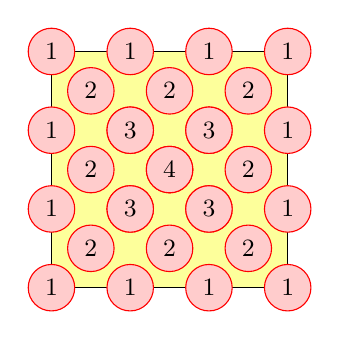
\begin{tikzpicture}[scale=0.5]
\draw[style=black] (3,3) to (-3,3) to (-3,-3) to (3,-3) to cycle;
\foreach \x in {0,1,2,3}{
    \foreach \y in {0,1,2,3}{
        \node[style=sred] at (3-2*\x,3-2*\y) {\small 1}; 
}}
\foreach \x in {0,1,2}{
    \foreach \y in {0,1,2}{
        \node[style=sred] at (2-2*\x,2-2*\y) {\small 2}; 
}}	
\foreach \x in {0,1}{
    \foreach \y in {0,1}{
        \node[style=sred] at (1-2*\x,1-2*\y) {\small 3}; 
}}	
\foreach \x in {0}{
    \foreach \y in {0}{
        \node[style=sred] at (0-2*\x,0-2*\y) {\small 4}; 
}}
 \end{tikzpicture}
 \end{center}
  \caption{The weight multiplicities of the crystal $B_3$.}
  \label{figurewts}
\end{figure}
\section{Swappable edges and their classification}

\subsection{Twisted Bruhat graphs}

The Bruhat order on the weight lattice $X$ is the order generated by the following relations

	
\begin{equation}\label{bruhatorder}s_\alpha^\vee(\lambda)< \lambda \iff \begin{cases}\langle \lambda,\beta^\vee\rangle > M &\text{if }M\geq 0,\\
\langle \lambda,\beta^\vee\rangle <  M&\text{if }M<0.\end{cases}\end{equation}
where $\alpha^\vee=M\delta+\beta^\vee$, with $\beta^\vee\in \Phi_+^\vee$ and $\lambda\in X$. The set of elements smaller that $\lambda$ in the Bruhat order, which we denote by $\{\leq \lambda\}$, can be characterized as
\begin{equation}\label{smallerthanlam}
    \{\leq \lambda\} =\Conv(W\cdot \lambda)\cap (\lambda+\bbZ\Phi)
\end{equation}
(see for example \cite[Chap. VIII, §7, exerc. 1]{Bou78}).

Let $\lambda\in X_+$. Let $\Gamma_\lambda$ denote the moment graph of the Schubert variety $\sch{\lambda}$. This is a directed labeled graph, also called the \emph{Bruhat graph} of $\lambda$. We recall  from \cite[\S 2.3]{Pat} the explicit description of $\Gamma_\lambda$.
The vertices of the graph $\Gamma_\lambda$ are all the weights in $\{\leq \lam\}$. We have an edge $\mu_1\raw \mu_2$ in $\Gamma_\lambda$ if and only if $\mu_2-\mu_1$ is a multiple of a root $\beta\in \Phi$ and $\mu_1\leq \mu_2$. In this case, the label of the edge $\mu_1\raw \mu_2$ is $m\delta-\beta^\vee$, where
\[m =-\frac{\langle \beta^\vee,\mu_1+\mu_2\rangle}{2}\] (cf. \cite[Lemma 2.6]{Pat}).  Notice that $s_{m\delta-\beta^\vee}(\mu_1)=\mu_2$. We denote by $E(\lambda)$ the set of edges in $\Gamma_\lam$.

Let $\Gamma_X$ denote the union of all the graphs $\Gamma_{\lambda}$, for $\lambda\in X_+$ (where $\Gamma_{\lambda}$ is regarded as a subgraph of $\Gamma_{\lambda'}$ if $\lambda\leq \lambda'$) and call it the Bruhat graph of $X$.





For $w\in \affW$ we denote by \[N(w):=\{\alpha \in \affPhi^\vee_+\mid w^{-1}(\alpha)\in \affPhi^\vee_-\}\] the set of inversions.
If $w=s_{i_1}\ldots s_{i_k}$ is a reduced expression for $w$ then \[N(w)=\{\alpha^\vee_{i_1},s_{i_1}(\alpha^\vee_{i_2}),\ldots,s_{i_1}s_{i_2}\ldots s_{i_{k-1}}(\alpha^\vee_{i_k})\}.\] 

We say that $w=s_1s_2\ldots s_k\ldots$ is a reduced infinite expression if for any $j$  the starting expression $w_j:=s_1s_2\ldots s_j$ is reduced.
If $w$ is a reduced infinite expression, let $N(w)=\bigcup_{j=1}^\infty N(w_j)$.


Consider $\undc = s_0s_2s_1s_2$. Then $y_\infty:=\undc \undc \undc\ldots$ is an infinite reduced expression.
Let $y_m$ be the element given by the first $m$ simple reflections in $y_{\infty}$.
We order the roots in $N(y_\infty)$ as follows:
\begin{multline}\label{reflectionorder}
\delta-\alpha_{21}^\vee<\delta-\alpha_{12}^\vee<2\delta-\alpha_{21}^\vee<  \delta -\alpha_{2}^\vee< 3\delta-\alpha_{21}^\vee<2\delta-\alpha_{12}^\vee< \\
\ldots<M\delta-\alpha_{12}^\vee<2M\delta-\alpha_{21}^\vee<M\delta-\alpha_{2}^\vee<(2M+1)\delta-\alpha_{21}^\vee<\ldots    
\end{multline}
so that the first $m$ roots in \eqref{reflectionorder} are precisely the elements of $N(y_m)$.

%We just write $\ell_m$ and $\leq_m$ for $\ell_{N(y_m)}$ and $\leq_{N(y_m)}$, the $y_m$-twisted length and the $y_m$-twisted Bruhat order on $\affW$.


	We define the \emph{$m$-twisted Bruhat order} $\leq_m$ of $\extW$ by setting 
	\[v\leq_m w\text{ if and only if }y_m^{-1}v\leq y_m^{-1}w,\]
	and the $m$-twisted length by $\ell_m(v):=\ell(y_m^{-1}v)$. 
Recall that $X\cong \extW/W$. Hence, the twisted Bruhat order on $\extW$ also induces a twisted Bruhat order on $X$. Concretely, this means that we regard $\lambda\in X$ as a right coset in $\extW$ and denote by $\lambda_m\in \extW$ the element of minimal $y_m$-twisted length in the coset $\lambda$. Then we set $\ell_m(\lambda):=\ell_m(\lambda_m)$ and $\mu\leq_m \lambda$ if $\lambda_m\leq_m \mu_m$.


	For every $m\in \bbZ_{\geq 0}$ we define $\Gamma_\lambda^m$, the $y_m$\emph{-twisted Bruhat graph of} $\lambda$, to be the directed labeled graph with the same vertices of $\Gamma_{\lambda}$ and where there is an edge $\mu\ra \lambda$ if there exists $\alpha^\vee\in \affPhi^\vee$ such that $s_{\alpha^\vee}(\mu)=\lambda$ and $\mu<_m \lambda$. Concretely, we can obtain $\Gamma_\lambda^m$ from $\Gamma_{\lambda}$ by inverting the orientation of all the arrows in $\Gamma_\lambda$ with label in $N(y_m)$.
	
	Since each graph $\Gamma_{\lambda}$ has only a finite number of edges, the twisted graphs $\Gamma_{\lambda}^m$ stabilize for $m$ big enough, so we can define $\Gamma_{\lambda}^\infty:=\Gamma_{\lambda}^m$ for $m\gg 0$. 

For $m\in \bbZ_{\geq 0} \cup \{\infty\}$, we define $\Gamma^m_X$ as the union of all the graphs $\Gamma^m_\lambda$, for $\lambda\in X_+$. The graph $\Gamma^m_X$ can be obtained from $\Gamma_X$ by inverting the orientation of all the arrows with label in $N(y_m)$.



\begin{definition} 
\label{twistedarrowslambdamu}
	For $\mu\leq \lambda$, we denote by $\Arr_m(\mu,\lam)$ the set of arrows pointing to $\mu$ in $\Gamma_m^\lambda$ and by $\ell_m(\mu,\lambda):=|\Arr_m(\mu,\lam)|$ the number of those arrows. 
	
	For $i \in \{1,2,21,12\}$ let $\Arr_m^{i}(\mu,\lam)$ be arrows pointing to $\mu$ in $\Gamma_m^\lambda$ of the form $\mu-k\alpha_i\raw \mu$ for $k\in \bbZ$. Let $\ell_m^i(\mu,\lam)=|\Arr_m^{i}(\mu,\lam)|$.
	
	Let $\Arr_\mu(\mu)$ be the set of arrows pointing to $\mu$ in $\Gamma_X^m$. For $i\in \{1,2,21,12\}$, the set $\Arr_m^i(\mu)$ is defined accordingly.
\end{definition}

Recall from \cite[Lemma 4.6]{Pat} that $|\Arr_m(\mu)|=\ell_m(\mu)$. We have 
\begin{equation}\label{ellsubdivided} \Arr_m(\mu,\lambda)=\bigcup_{i\in \{1,2,12,21\}}\Arr_m^i(\mu,\lambda)\quad\text{and}\quad
\ell_m(\mu,\lambda)=\sum_{i\in \{1,2,12,21\}} \ell_m^i(\mu,\lam)
 \end{equation}
 for any $\mu\leq \lambda$. Notice that, since there are no arrows in $N(y_\infty)$ of the form $M\delta-\alpha_1^\vee$, the set $\Arr_m^1(\mu,\lambda)$ does not depend on $m$, and does not depend on $\lambda$ as long as $\mu\leq \lambda$. If $\mu \leq \lambda$, for all $m$ by \eqref{bruhatorder} we have 
 \begin{align*}
 \Arr_m^1(\mu,\lambda)&=\{\mu - k\alpha_1\ra \mu \mid \mu-k\alpha_1\leq \mu\}\\
 &=\begin{cases}
 \{\mu - k\alpha_1\ra \mu \mid 0<k\leq \mu_1\}&\text{if }\mu_1\geq 0\\
 \{\mu - k\alpha_1\ra \mu \mid 0>k>\ \mu_1\}&\text{if }\mu_1< 0.
 \end{cases}
 \end{align*}
Hence, we have  \begin{equation}\label{ell1}\ell_m^1(\mu,\lam)=\begin{cases} \mu_1 &\text{if }\mu_1\geq 0\\
-\mu_1-1& \text{if }\mu_1<0.\end{cases}\end{equation}


\subsection{Swappable edges}

To pass from $\Gamma^m_\lambda$ to $\Gamma^{m+1}_\lambda$ (and from $\Gamma^m_X$ to $\Gamma^{m+1}_X)$ we need to invert the arrows with label $\alpha^\vee_{t_{m+1}}$, where $t_{m+1}$ is the reflection \begin{equation}\label{tm}t_{m+1}:=y_{m+1}y_m^{-1} =y_ms'_{m+1} y_m^{-1}.
\end{equation}
Here $s'_{m+1}$ denotes the $(m+1)$-th simple reflection in $y_\infty$.
Notice that $\{\alpha^\vee_{t_{m+1}}\}= N(y_{m+1})\setminus N(y_m)$.


If $\mu < t_{m+1}\mu$, then $\Arr_{m+1}(t_{m+1}\mu)\setminus \Arr_m(t_{m+1}\mu)=\{\mu\raw t_{m+1} \mu\}$ and $\Arr_{m}(\mu)$ is in bijection with $\Arr_{m}(t_{m+1}\mu)\setminus \{\mu\raw t_{m+1}\mu\}$ by \cite[Lemma 4.8]{Pat}. In particular, we have 
\begin{equation}\label{lmX}
\ell_m(\mu)=\ell_m(t_{m+1}\mu)-1.
\end{equation}



A remarkable property of the twisted Bruhat graphs in type $A$ (\cite[Prop. 4.14]{Pat}) is that the same is true if we restrict to $\Gamma_\lambda$, i.e. $\ell_m(\mu,\lambda)=\ell_m(t_{m+1}\mu,\lambda)-1$ if $\mu <t_{m+1}\mu \leq \lambda$. This implies that
$\ell_{m+1}(\mu,\lambda)=\ell_m(t_{m+1}\mu,\lambda)$ and $\ell_m(\mu,\lam)=\ell_{m+1}(t_{m+1}\mu,\lam)$. However, as we will see in \Cref{exampleswap}, this property does not hold in type $C_2$. The goal of this section is to classify the set of edges for which it holds.


\begin{definition}
\label{def:swappableedge}
	We say that an edge $\mu \raw t_{m+1}\mu$ in $\Gamma_{\lambda}$ is \emph{swappable} if 
 \begin{equation}\label{eqswapdef}
 \ell_m(\mu,\lambda)= \ell_m(t_{m+1}\mu,\lambda)-1.
 \end{equation}
 We also say that an edge is \emph{NS} if it is not swappable.
	We denote by $E^S(\lambda)$ and $E^N(\lambda)$ the sets of swappable and non-swappable edges in $\Gamma_\lambda$, respectively. 
\end{definition}


As it turns out, to determine if an edge is swappable or not, we have to solve an elementary geometric problem,  as the next example illustrates.

%We denote an element $\nu\in X$ as $\nu=(\nu_1,\nu_2)$, where
%$\nu_1:=\langle \nu,\alpha_1^\vee\rangle$ and $\nu_2:=\langle \nu,\alpha_2^\vee\rangle$ so that $\nu=\nu_1 \varpi_1 + \nu_2 \varpi_2 $. Note that this is not the same as the notation for the corresponding partition. %which would correspond to $(\nu_{1}+\nu_{2},\nu_{2})$.


\begin{example}\label{exampleswap}
In the \Cref{figswapp,fignonswapp} the starting points of the arrows in $\ell_m(\mu,\lam)$ are denoted by red circles while the starting points of the arrows in $\ell_m(t_{m+1}\mu,\lam)$ are denoted by blue squares. 

Assume that $\lambda=(2,2)$, $\mu=(2,-1)$ and that $m+1=8$, i.e. that $t:=t_{m+1}$ is the reflection corresponding to the root $2\delta-\alpha_2^\vee$.
In \Cref{figswapp}, the yellow octagon is the convex hull of $W\cdot \lambda$ while the green octagon is (the border of) the convex hull of $y_mWy_m^{-1}\cdot \mu$. As we will observe in \Cref{sec:twistedreflection}, the arrows in $\Arr_m(\mu,\lam)$ and $\Arr_m(t_{m+1}\mu,\lam)$ can be characterized as the weights in the diagonal of the green octagon which lie inside the yellow octagon. In this case we see that there are 
are $7$ red dots and $8$ blue squares, meaning that  the edge $\mu\raw t\mu$ is swappable. 


Now assume that $\lam=(2,2)$, $\mu=(4,-2)$ and $m+1=12$, i.e. that $t:=t_{m+1}=s_{3\delta-\alpha_2^\vee}$. As illustrated in \Cref{fignonswapp}, we have $9$ red dots and $9$ blue squares, so in this case the edge $\mu\raw t\mu$ is not swappable.


\begin{figure}
\centering
\begin{minipage}{.5\textwidth}
  \centering
	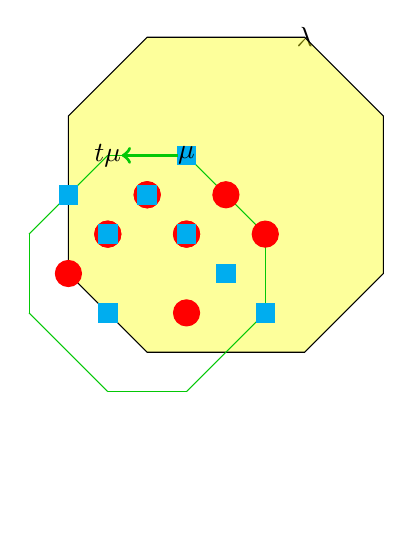
\begin{tikzpicture}[scale=0.5]
 \node [style=none] (0) at (-2, 4) {};
	\node [style=none] (3) at (2, 4) {$\lambda$};
	\node [style=none] (4) at (-4, 2) {};
	\node [style=none] (5) at (4, 2) {};
	\node [style=none] (6) at (4, -2) {};
	\node [style=none] (7) at (2, -4) {};
	\node [style=none] (8) at (-4, -2) {};
	\node [style=none] (9) at (-2, -4) {};
	\node [style=none] (10) at (-1, 1) {};
	\node [style=none] (11) at (-3, 1) {};
	\node [style=none] (12) at (1, -1) {};
	\node [style=none] (13) at (1, -3) {};
	\node [style=none] (14) at (-1, -5) {};
	\node [style=none] (15) at (-3, -5) {};
	\node [style=none] (17) at (-5, -3) {};
	\node [style=none] (18) at (-5, -1) {};
 	\draw [style=black] (5.center) 	to (3.center) to (0.center) to (4.center) to (8.center) to (9.center) to (7.center) to (6.center) to cycle;
	\draw [style=green] (11.center) to (10.center);
	\draw [style=green] (10.center) to (12.center);
	\draw [style=green] (12.center) to (13.center);
	\draw [style=green] (13.center) to (14.center);
	\draw [style=green] (14.center) to (15.center);
	\draw [style=green] (15.center) to (17.center);
	\draw [style=green] (17.center) to (18.center);
	\draw [style=green] (18.center) to (11.center);
	\node [style=blue] (35) at (-1, 1) {};

	\node [style=none] (19) at (-1, 1) {$\mu$};
	\node [style=red] (20) at (-1, -1) {};
	\node [style=red] (21) at (-1, -3) {};
	\node [style=red] (22) at (-2, 0) {};
	\node [style=red] (23) at (-3, -1) {};
	\node [style=red] (24) at (-4, -2) {};
	\node [style=red] (25) at (0, 0) {};
	\node [style=red] (26) at (1, -1) {};
	\node [style=none] (27) at (-3, 1) {$t\mu$};
	\node [style=red] (36) at (-2, 0) {};
	\node [style=red] (37) at (-1, -1) {};
	\node [style=red] (29) at (-3, -1) {};
	\node [style=blue] (28) at (-3, -1) {};
	\node [style=blue] (30) at (-2, 0) {};
	\node [style=blue] (31) at (-1, -1) {};
	\node [style=blue] (32) at (0, -2) {};
	\node [style=blue] (33) at (1, -3) {};
	\node [style=blue] (34) at (-3, -3) {};
	\node [style=blue] (35) at (-4, 0) {};
    \node at (0,-8) {};
    \draw[green, very thick, ->] (19) to (27);
	\end{tikzpicture}
 \captionof{figure}{A swappable edge}
  \label{figswapp}
\end{minipage}%
\begin{minipage}{.5\textwidth}
  \centering
  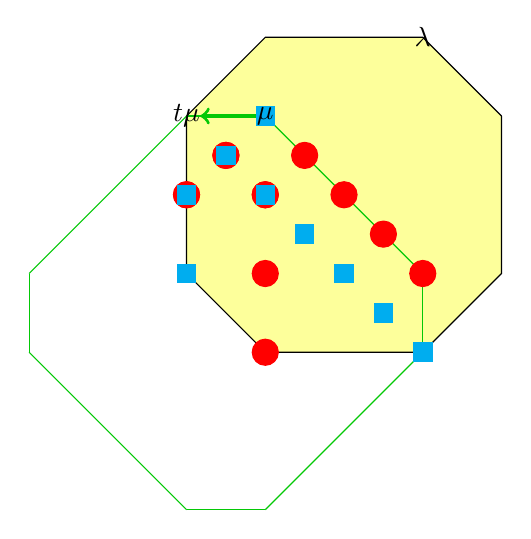
\begin{tikzpicture}[scale=0.5]
		\begin{pgfonlayer}{nodelayer}
			\node [style=blue] (40) at (-2,2) {};
			\node [style=none] (0) at (-2, 4) {};
			\node [style=none] (3) at (2, 4) {$\lambda$};
			\node [style=none] (4) at (-4, 2) {};
			\node [style=none] (5) at (4, 2) {};
			\node [style=none] (6) at (4, -2) {};
			\node [style=none] (7) at (2, -4) {};
			\node [style=none] (8) at (-4, -2) {};
			\node [style=none] (9) at (-2, -4) {};
			\node [style=none] (10) at (-2, 2) {};
			\node [style=none] (11) at (-4, 2) {};
			\node [style=none] (12) at (2, -2) {};
			\node [style=none] (13) at (2, -4) {};
			\node [style=none] (14) at (-2, -8) {};
			\node [style=none] (15) at (-4, -8) {};
			\node [style=none] (17) at (-8, -4) {};
			\node [style=none] (18) at (-8, -2) {};
			\node [style=none] (19) at (-2, 2) {$\mu$};
			\node [style=red] (20) at (-2, 0) {};
			\node [style=red] (21) at (-2, -2) {};
			\node [style=red] (22) at (-3, 1) {};
			\node [style=red] (23) at (-4, 0) {};
			\node [style=red] (24) at (-2, -4) {};
			\node [style=red] (25) at (-1, 1) {};
			\node [style=red] (26) at (0, 0) {};
			\node [style=none] (27) at (-4, 2) {$t\mu$};
			\node [style=red] (29) at (-4, 0) {};
			\node [style=blue] (28) at (-4, 0) {};
			\node [style=red] (36) at (-3, 1) {};
			\node [style=red] (37) at (-2, 0) {};
			\node [style=red] (38) at (1, -1) {};
			\node [style=red] (39) at (2, -2) {};
			\node [style=blue] (40) at (1, -3) {};
			\node [style=blue] (41) at (2, -4) {};
			\node [style=blue] (30) at (-3, 1) {};
			\node [style=blue] (31) at (-2, 0) {};
			\node [style=blue] (32) at (-1, -1) {};
			\node [style=blue] (33) at (0, -2) {};
			\node [style=blue] (34) at (-4, -2) {};
            \draw[green, very thick, ->] (19) to (27);

		\end{pgfonlayer}
		\begin{pgfonlayer}{edgelayer}
			\draw [style=black] (5.center)
			to (3.center)
			to [in=0, out=180] (0.center)
			to (4.center)
			to (8.center)
			to (9.center)
			to (7.center)
			to (6.center)
			to (5.center);
			\draw [style=green] (11.center) to (10.center);
			\draw [style=green] (10.center) to (12.center);
			\draw [style=green] (12.center) to (13.center);
			\draw [style=green] (13.center) to (14.center);
			\draw [style=green] (14.center) to (15.center);
			\draw [style=green] (15.center) to (17.center);
			\draw [style=green] (17.center) to (18.center);
			\draw [style=green] (18.center) to (11.center);
		\end{pgfonlayer}
  	\end{tikzpicture}
  \captionof{figure}{A non-swappable edge}
  \label{fignonswapp}
\end{minipage}
\end{figure}



\end{example}

\subsection{Geometry of atoms}

We fix $\lambda\in X_+$. Recall that $\label{leqlambda} \{\leq\lambda\}=(\lambda+\bbZ\Phi) \cap \Conv(W\cdot \lambda).$
%In other words,  $\{\leq \lambda \}$ is the set of all the weights $\mu$ lying in the same class of $\lambda$ in $X/\bbZ\Phi$ and belonging to the polytope $\Conv(W\cdot \mu)$.
In our situation, the convex hull $\Conv(W\cdot \mu)$ is an octagon with vertices as in \Cref{figoctagon}. We can make the actual conditions more explicit.


\begin{figure}[hbt!]
\begin{center}
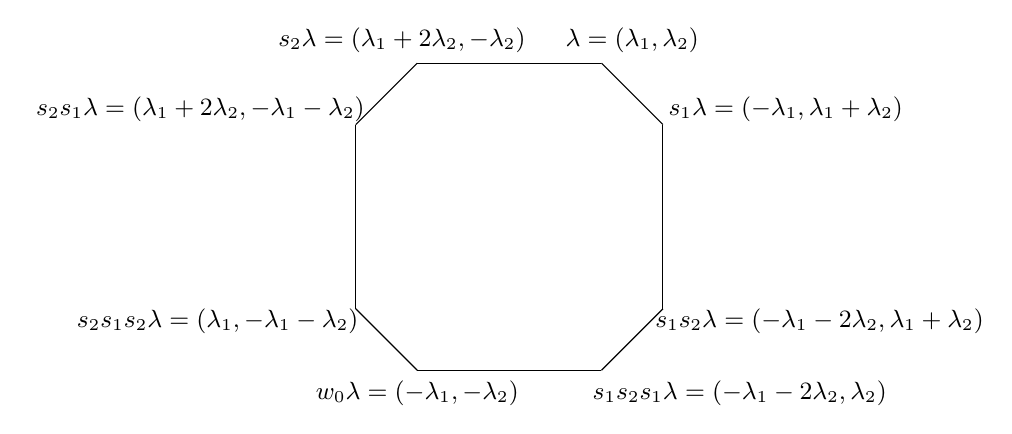
\begin{tikzpicture}[scale=0.39]
\begin{pgfonlayer}{nodelayer}
\node [style=none] (0) at (3, 5) {};
\node [style=none] (1) at (5, 3) {};
\node [style=none] (2) at (5, -3) {};
\node [style=none] (3) at (-3, 5) {};
\node [style=none] (4) at (-5, 3) {};
\node [style=none] (5) at (-5, -3) {};
\node [style=none] (6) at (-3, -5) {};
\node [style=none] (7) at (3, -5) {};
\node [style=none] (8) at (2, 4.25) {};
\node [style=none] (9) at (2, 4.25) {};
\node [style=none] (10) at (2, 4.25) {};
\node [style=none] (11) at (4, 5.75) {\small{$\lambda=(\lambda_1,\lambda_2)$}};
\node [style=none] (13) at (-10.2, 3.5) {      \small{ $s_2s_1\lambda = (\lambda_1+2\lambda_2,-\lambda_1-\lambda_2)$}};
\node [style=none] (14) at (-9.5, -3.4) {\small{$s_2s_1s_2\lambda=(\lambda_1,-\lambda_1-\lambda_2)$}};
\node [style=none] (15) at (-3, -5.75) {\small{$w_0\lambda=(-\lambda_1,-\lambda_2)$}};
\node [style=none] (16) at (7.5, -5.75) {\small{$s_1s_2s_1\lambda=(-\lambda_1-2\lambda_2,\lambda_2)$}};
\node [style=none] (17) at (10.1, -3.4) {\small{$s_1s_2\lambda=(-\lambda_1-2\lambda_2,\lambda_1+\lambda_2)$}};
\node [style=none] (18) at (9, 3.5) {\small{$s_1\lambda=(-\lambda_1,\lambda_1+\lambda_2)$}};
\node [style=none] (19) at (-3.5, 5.75) {\small{$s_2\lambda=(\lambda_1+2\lambda_2,-\lambda_2)$}};
\end{pgfonlayer}
\begin{pgfonlayer}{edgelayer}
\draw (4.center) to (5.center);
\draw (5.center) to (6.center);
\draw (6.center) to (7.center);
\draw (7.center) to (2.center);
\draw (2.center) to (1.center);
\draw (1.center) to (0.center);
\draw (0.center) to (3.center);
\draw (3.center) to (4.center);
\end{pgfonlayer}
\end{tikzpicture}
\end{center}
\caption{The $W$-orbit and the convex hull of $\lambda$}\label{figoctagon}
\end{figure}


\begin{lemma}
\label{octineq}
We have $\mu\leq \lambda$ if and only if $\mu_1\equiv \lam_1 \pmod{2}$ and the following inequalities hold:
\begin{alignat*}{4}
    &-\lam_1-2\lam_2 	&&\leq \mu_1 &&=\langle \mu,\alpha_1^\vee\rangle &&\leq \lam_1+2\lam_2\\
    &-\lam_1-\lam_2 	&&\leq \mu_1+\mu_2 &&=\langle \mu,\alpha_{12}^\vee\rangle &&  \leq  \lam_1+\lam_2\\
    &-\lam_1-\lam_2	&&\leq\mu_2 &&=\langle \mu,\alpha_2^\vee\rangle&&  \leq \lam_1+\lam_2\\
    &-\lam_1-2\lam_2	&&\leq\mu_1+2\mu_2&&=\langle \mu,\alpha_{21}^\vee\rangle &&   \leq \lam_1+2\lam_2.
\end{alignat*}

\end{lemma}
\begin{proof}
	 It is easy to see that $\mu \equiv \lambda \pmod{\bbZ \Phi}$ if and only if $\mu_1=\lambda_1$. The inequalities can be easily deduced from \Cref{figoctagon}
\end{proof}




We introduce now some helpful quantities which evaluate the distance of a weight $\mu$ from the walls of $\Conv(W\cdot \lambda)$.

\begin{definition}\label{affphidef}
	For $i\in \{1,2,21,12\}$, let $\affphi_i(\mu,\lambda)$ be the maximum integer $k$ such that $\mu-k\alpha_i\leq \lambda$. 
\end{definition}

\begin{lemma}\label{affphicompute}
	Let $\mu\leq \lambda$. We have
	\begin{enumerate}
		\item 
		$
		\affphi_{21}(\mu,\lambda)= \lam_2+\mu_2+\min\left(\lam_1,\frac{\lam_1+\mu_1}{2},\lam_1+\mu_1\right) $   
		%		= &    \begin{cases}
		%		\lambda_1+\lambda_2+\mu_2 &\text{if }\mu_1\geq \lambda_1\\
		%		\frac{\lambda_1+\mu_1}{2}+\lambda_2+\mu_2&\text{if }-\lambda_1\leq \mu_1\leq \lambda_1 \\
		%		\lambda_1+\lambda_2+\mu_1+\mu_2 &\text{if }\mu_1\leq -\lambda_1\\
		%		\end{cases}\end{align*}
		\item $		\affphi_{12}(\mu,\lambda)= \frac{\lambda_1+\mu_1}{2} +\min\left(\lambda_2+\mu_2,\lfl\frac{\lambda_2+\mu_2}{2}\rfl,\lambda_2\right)$ 
		
		%		&\begin{cases}
		%			
		%		\frac{\lambda_1+\mu_1}{2} + \lambda_2+\mu_2 &\text{if }\mu_2\leq -\lambda_2\\
		%		\frac{\lambda_1+\mu_1}{2}+\lfl\frac{\lam_2+\mu_2}{2}\rfl&\text{if }-\lambda_2\leq\mu_2\leq \lambda_2 \\
		%		\frac{\lambda_1+\mu_1}{2} + \lambda_2 &\text{if }\mu_2\geq \lambda_2\\
		%		\end{cases}\end{align*}
		\item $\affphi_{2}(\mu,\lambda):=\frac{\lambda_1-\mu_1}{2} +\min\left(\lambda_2+\mu_1+\mu_2,\lfl\frac{\lambda_2+\mu_1+\mu_2}{2}\rfl,\lambda_2\right).$	
	\end{enumerate}
	
\end{lemma}
\begin{proof}
	We prove only the first statement, since the other two are analogous. 
	Consider the maximal $x\in \mathbb{R}_{\geq 0}$ such that $\nu:=\mu-x\alpha_{21}\in \Conv(W\cdot \lambda)$. Then $\mu-x\alpha_{21}$ belongs to the boundary of $\Conv(W\cdot \lambda)$ and $\affphi_{21}(\mu,\lambda)=\lfloor x \rfloor$. 
	
	We have $(\nu_1,\nu_2)=(\mu_1,\mu_2-x)$, hence by \Cref{octineq} the following inequalities three inequalities hold
	\begin{align*}
	-\lam_1-\lam_2 \leq &\; \mu_1 +\mu_2-x\\
	-\lam_1-\lam_2\leq &\;\mu_2-x\\
	-\lam_1 -2 \lam_2 \leq&\; \mu_1+2\mu_2-2x	
	\end{align*} 
	and since we are on the boundary at least one of them must be an equality. It follows that
\begin{align*}
x &= \min(\mu_1+\mu_2+\lam_1+\lam_2,\lam_1+\lam_2+\mu_2,\frac{\lam_1+\mu_1}{2} + \lam_2+\mu_2)\\
  &= \lam_2+\mu_2+\min(\lam_1,\frac{\lam_1+\mu_1}{2},\lam_1+\mu_1).\qedhere
\end{align*}
	
%	If $z,z'\in X_\bbR$, we denote by $[z,z']$ the segment between them.
%	The weight $\nu$ belongs to one among the segments $[s_2s_1\lambda,s_2s_1s_2\lambda]$,  $[s_2s_1s_2\lambda,s_1s_2s_1s_2\lambda]$ and  $[w_0\lambda,s_1s_2s_1\lambda]$.
%	We consider these three cases separately. 
%	
%	
%	
%	Assume first $\nu \in [s_2s_1\lambda,s_2s_1s_2\lambda]$. We have $s_2s_1\lambda=(\lambda_1+2\lambda_2,-\lambda_1-\lambda_2)$ and $s_2s_1s_2\lambda=(\lambda_1,-\lambda_1-\lambda_2)$. It follows that  $\nu_2=-\lambda_1-\lambda_2$ and 
%	$\lambda_1\leq \nu_1\leq \lambda_1+2\lambda_2$. Hence $\lambda_1\leq \mu_1\leq \lambda_1+2\lambda_2$ and $x=\lambda_1+\lambda_2+\mu_2$. 
%	
%	
%	Assume we are in the second case. We have $w_0\lambda=-\lambda=(-\lambda_1,-\lambda_2)$. So we have
%	$\nu_1+2\nu_2=-\lambda_1-2\lambda_2$ and $-\lambda_1\leq \nu_1\leq \lambda_1$. We get $\mu_1+2\mu_2-2x=-\lambda_1-2\lambda_2$. Hence $x=\frac{\lambda_1+\mu_1}{2}+\lambda_2+\mu_2$. 
%	
%	Similarly, in the third case, we have $\nu_1+\nu_2=-\lambda_1-\lambda_2$, hence $x=\lambda_1+\lambda_2+\nu_1+\nu_2$.
\end{proof} 


\subsection{Twisted Reflection Groups}
\label{sec:twistedreflection}

%Recall from  \cite[Lemma 4.2]{Pat} that $\ell_m(\mu)=\ell_m(v\mu)-1$, and an explicit bijection between the arrows is obtained by  conjugating by $t$.



For $k\geq 0$ consider the reflection subgroup \[ W^{k}:=y_{k}Wy_{k}^{-1}\subset \affW.\]
Note that for any $k$ we have 
$W^{k+1}=t_{k+1}W^k t_{k+1}$.

\begin{lemma}
\label{twistedweylgroups}
For any $M>0$ we have 
$W^{4M-3}=W^{4M-2}=W^{4M-1}=W^{4M}$. Moreover, the reflections in $W^{4M}$ correspond to the roots
 \[\{\alpha_1^\vee,M\delta-\alpha_2^\vee,M\delta-\alpha_{12}^\vee,2M\delta-\alpha_{21}^\vee\}.\]
\end{lemma}
\begin{proof}
We check this by induction. Recall that for any $M>0$, $t_{4M-3}$, $t_{4M-2}$, $t_{4M-1}$, and $t_{4M}$ are the reflections corresponding to the roots $(2M-1)\delta-\alpha_{21}^\vee$,
$M\delta-\alpha_{12}^\vee$, $2M\delta-\alpha_{21}^\vee$, and $M\delta-\alpha_2^\vee$, respectively. 

Recall that for any $M\in \bbN$ we have
\[W^{4M-3}=t_{4M-3}W^{4M-4}t_{4M-3}.\] 

By induction, the reflections in $W^{4M-4}$ correspond to the roots $\alpha^\vee_{1}, (M-1)\delta -\alpha_{2}^\vee , (M-1)\delta -\alpha_{12}^\vee$, and $2(M-1)\delta - \alpha_{21}^\vee$. 



The claim follows since
\begin{align*}
   s_{(2M-1)\delta-\alpha_{21}^\vee}(\alpha_1^\vee)&=\alpha_1^\vee\\
s_{(2M-1)\delta-\alpha_{21}^\vee}((M-1)\delta-\alpha_2^\vee)&=-M+\alpha_{12}^\vee\\ s_{(2M-1)\delta-\alpha_{21}^\vee}((M-1)\delta-\alpha_{12}^\vee)&=-M+\alpha_{2}^\vee\\ s_{(2M-1)\delta-\alpha_{21}^\vee}(2(M-1)\delta-\alpha_{21}^\vee)&=-2M\delta+\alpha_{21}^\vee ,
\end{align*}
therefore $t_{4M-i} \in W^{4M-3}$ for $0 \leq i \leq 3$, which implies that 

\[W^{4M}=W^{4M-1}=W^{4M-2}=W^{4M-3}. \qedhere \]
\end{proof}


The set of reflections in $W^{4M}$ is $\{s_1, v_M, q_M, r_M\}$, where $v_M$, $q_M$ and $r_M$ are the reflection  corresponding to the roots $M\delta-\alpha_2^\vee,M\delta-\alpha_{12}^\vee,2M\delta-\alpha_{21}^\vee$, as depicted in \Cref{Wmu}. More explicitly, we have
 \begin{alignat}{3}\label{vMmu}
 &v_M\mu &&=\mu-(\mu_2+M)\alpha_{2} &&=(\mu_1+2\mu_2+2M,-\mu_2-2M) \\
  &q_M\mu &&= \mu-(\mu_1+\mu_2+M)\alpha_{12} &&=(-\mu_1-2\mu_2-2M,\mu_2)\\
 &	r_M\mu  &&=\mu-(\mu_1+2\mu_2+2M)\alpha_{21} &&= (\mu_1,-\mu_1-\mu_2-2M)
 \end{alignat}
We also have $q_M=s_1v_Ms_1$ and $r_M=v_Ms_1v_M$.


\begin{figure}
	\begin{center}
	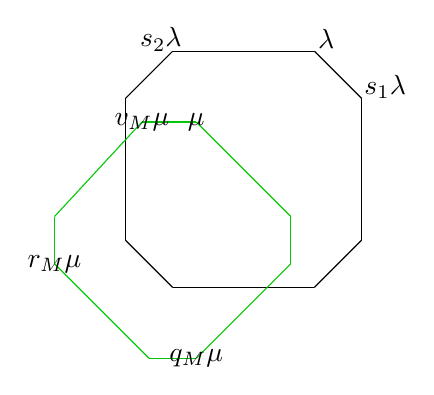
\begin{tikzpicture}[scale=0.3]
	\begin{pgfonlayer}{nodelayer}
	\node [style=none] (20) at (-2, 2) {$\mu$};
	\node [style=none] (21) at (-4.3, 2) {$v_M\mu$};
	\node [style=none] (22) at (2, -2) {};
	\node [style=none] (23) at (2, -4) {};
	\node [style=none] (24) at (-2, -8) {$q_M\mu$};
	\node [style=none] (25) at (-4, -8) {};
	\node [style=none] (27) at (-8, -4) {$r_M\mu$};
	\node [style=none] (28) at (-8, -2) {};
	
	\node [style=none] (0) at (3, 5) {};
	\node [style=none] (1) at (5, 3) {};
	\node [style=none] (2) at (5, -3) {};
	\node [style=none] (3) at (-3, 5) {};
	\node [style=none] (4) at (-5, 3) {};
	\node [style=none] (5) at (-5, -3) {};
	\node [style=none] (6) at (-3, -5) {};
	\node [style=none] (7) at (3, -5) {};
	\node [style=none] (8) at (2, 4.25) {};
	\node [style=none] (9) at (2, 4.25) {};
	\node [style=none] (10) at (2, 4.25) {};
	\node [style=none] (11) at (3.5, 5.5) {$\lambda$};
	\node [style=none] (18) at (6, 3.5) {$s_1\lambda$};
	\node [style=none] (19) at (-3.5, 5.5) {$s_2\lambda$};
	\end{pgfonlayer}
	\begin{pgfonlayer}{edgelayer}
	\draw (4.center) to (5.center);
	\draw (5.center) to (6.center);
	\draw (6.center) to (7.center);
	\draw (7.center) to (2.center);
	\draw (2.center) to (1.center);
	\draw (1.center) to (0.center);
	\draw (0.center) to (3.center);
	\draw (3.center) to (4.center);
	\end{pgfonlayer}
	\begin{pgfonlayer}{edgelayer}
	\draw [style=green] (21.center) to (20.center);
	\draw [style=green] (20.center) to (22.center);
	\draw [style=green] (22.center) to (23.center);
	\draw [style=green] (23.center) to (24.center);
	\draw [style=green] (24.center) to (25.center);
	\draw [style=green] (25.center) to (27.center);
	\draw [style=green] (27.center) to (28.center);
	\draw [style=green] (28.center) to (21.center);
	\end{pgfonlayer}
	\end{tikzpicture}
	\end{center}
	\caption{The green octagon is the border of the convex hull of $W^{4M}\cdot \mu$.}
	\label{Wmu}
\end{figure}

We can use the twisted reflection subgroups $W^m$ to describe the set of smaller elements with respect to twistet Bruhat order.

\begin{lemma}\label{leqmu}
Let $\mu\in X$.
\begin{enumerate}
    \item For any $m\geq 0$ we have $\{\leq_{m} \mu\}\subset \Conv(W^m\cdot \mu)$. 
    \item If $\mu_1\geq  0$ and $\mu\leq v_M\mu$, we have
	\[\{\leq_{4M} \mu\} 
	=\Conv(W^{4M} \cdot \mu)\cap (\mu+\bbZ\Phi)=\{\leq_{4M-1} v_M\mu\}\]
\end{enumerate}
\end{lemma}
\begin{proof}
Let $\nu\leq_{m} \mu$. Then $y_{m}^{-1}\nu\leq y_{m}^{-1}\mu$, so $y_{m}^{-1}\nu\in \Conv(W\cdot y_{m}^{-1}\mu)$. This shows the first part.
For the second part, because of \eqref{smallerthanlam},
it is enough to show that $y_{4M}^{-1}\mu=y_{4M-1}^{-1}v_M\mu$ is dominant, since then 
\[\{\leq_{4M} \mu\}=\{\leq_{4M-1} v_M\mu\}=\{\leq y_{4M}^{-1} \mu\} 
	=\Conv(W \cdot y_{4M}^{-1}\mu)\cap (\mu+\bbZ\Phi). \]

\noindent Recall that a weight $\tau \in X$ is dominant if and only if $\tau\geq s_1\tau$ and $\tau\geq s_2\tau$. We have $s_1\mu\leq \mu$, and this is equivalent to $s_1\mu\leq_{4M} \mu$. Moreover, $s_1$ commutes with $y_4$ and therefore also with $y_{4M}$. It follows that $s_1y_{4M}^{-1}\mu=y_{4M}^{-1}s_1\mu\leq  y_{4M}^{-1}\mu$.
	
We have $\mu \leq v\mu$, and this is equivalent to $v\mu\leq_{4M}\mu$, so $y_{4M}^{-1}\mu \geq y_{4M}^{-1}v\mu=y_{4M-1}^{-1}\mu=s_2y_{4M}^{-1}\mu$.
\end{proof}


Recall from \Cref{affphidef} the definition of $\affphi_i(\mu,\lambda)$.


\begin{lemma}\label{l=phi}
Assume that $\mu \leq v_M\mu$. Then we have
\begin{equation}\label{eqtu}v_M\mu \not\leq \lambda \iff M>\affphi_2(\mu,\lam)-\mu_2 \iff  \ell^2_{4M-1}(\mu,\lam)=\affphi_2(\mu,\lam),\end{equation}
\end{lemma}
\begin{proof}
    By \eqref{vMmu} and the definition of $\affphi_2$ we have $v_M\mu\leq \lam$ if and only if $\mu_2+M\leq \affphi_2(\mu,\lam)$.
    It follows from \Cref{leqmu}.2) that $\Arr_{4M}^2(\mu)$ consists precisely of the arrows $(\mu-k \alpha_2\raw \mu)$, with $\mu -k\alpha_2$ lying on the segment between $\mu$ and $v_M\mu$. In other words,  we have
\[ \Arr_{4M}^{2}(\mu)=\{(\mu-k\alpha_2 \raw \mu) \mid 1 \leq k \leq \mu_2 +M\}\]
If $v_M\mu\leq \lam$, then $\Arr_{4M}^2(\mu)=\Arr_{4M}^2(\mu,\lam)$, so \[\ell^2_{4M-1}(\mu,\lam)=\ell^2_{4M}(\mu,\lam)-1=\mu_2+M-1< \affphi_2(\mu,\lam).\] If $v_M\not \leq \lam$ we have \[\Arr_{4M}^2(\mu,\lam)=\{\{(\mu-k\alpha_2) \raw \mu \mid 1 \leq k \leq \affphi_2(\mu,\lam)\}\] and so $\ell^2_{4M-1}(\mu,\lam)=\ell^2_{4M}(\mu,\lam)= \affphi_2(\mu,\lam)$.
\end{proof}

Similarly, we have
\begin{itemize}
    \item $\displaystyle \Arr_{4M-2}^{12}(\mu)=\{(\mu-k\alpha_{12}) \raw \mu \mid 1 \leq k \leq \mu_1+\mu_2 + M\}.$ and if $\mu\leq q_M\mu$ we have 
\begin{equation}\label{eqqu} q_M\mu \not \leq \lambda \iff M> \affphi_{12}(\mu,\lambda)-\mu_1- \mu_2\iff \ell_{4M-3}^{12}(\mu,\lam)=\affphi_{12}(\mu,\lambda)
\end{equation}
\item $\displaystyle\Arr_{4M-1}^{21}(\mu)=\{(\mu-k\alpha_{21}) \raw \mu \mid 1 \leq k \leq \mu_1 + 2\mu_2 +2M\}$ and if $\mu\leq r_M\mu$ we have
\begin{equation}\label{eqru}
    r_M\mu \not \leq \lambda \iff 2M > \affphi_{21}(\mu,\lambda)-\mu_1 -2 \mu_2\iff \ell_{4M-2}^{21}(\mu,\lam)=\affphi_{21}(\mu,\lambda).
\end{equation} 
\end{itemize}


% We now prove the second equivalence. Notice that 
% \[\Arr_{\infty}(\mu,\lam)=\{ \mu -k\alpha_2\raw \mu \mid k>0\text{ and }\mu -k\alpha_2\leq \lam\},\]
% so $\ell^2_\infty(\mu,\lam)=\affphi_2(\mu,\lam)$. If $v_M\mu\not \leq \lam$ then $v_P\mu\not\leq \lam$ for all $P\geq M$ and so $\Arr_{4M-1}(\mu,\lam)=\Arr_\infty(\mu,\lam)$. If $v_M\mu \leq \lam$ then $(v_M\mu\raw \mu)\in \Arr^2_\infty(\mu,\lam)\setminus \Arr_{4M-1}^2(\mu,\lam)$ and so $\ell^2_{4M-1}(\mu,\lam)<\affphi_2(\mu,\lam)$.




In the following Lemma we describe the Bruhat order on a $W^{4M}$-orbit.

\begin{lemma}\label{bruhatorderWk}
%\Leo{Maybe it is a bit too little motivated to have this lemma here. Where is it needed?} \Jaz{Haven't fount it used yet. It's not tagged with Cref anywhere else in the paper. }\Leo{It is actually used in 4.21, and I have also used it to simplify the second part of 4.11} 
Let $\mu \in X$ and $v_M,r_M,q_M$ as before.
If $\mu < v_M\mu$ and $\mu_1\geq 0$ or if $\mu<q_M\mu$ and $\mu_1\leq 0$, then $v_M\mu\leq r_Mv_M\mu<r_M\mu$ and $q_M\mu < r_M\mu$.
%    \item If $\mu < q\mu$ and $\mu_1\geq 0$, then $r\mu >\mu$ and 
\end{lemma}
\begin{proof}
Assume first $\mu_1\geq 0$ and $\mu< v_M\mu$, so $\mu_2> -M$.
We have $\langle v_M\mu,\alpha_{21}^\vee\rangle=(v_M\mu)_1+2(v_M\mu_2)=\mu_1-2M\geq -2M$, so $r_Mv_M\mu \geq v_M\mu$ by \eqref{bruhatorder}. We have $q_Mr_M =r_Mv_M$ and
$\langle r_M\mu,\alpha_{12}^\vee\rangle=-\mu_1-\mu_2-2M<-M$ so $r_Mv_M\mu<r_M\mu$. Similarly, we have $\mu < q_M\mu \leq v_Mq_M\mu \leq s_1v_Mq_M\mu=r_M\mu$. 
The case $\mu_1\leq 0$ and $\mu<q_M\mu$ is similar.
\end{proof}


% Recall that $\nu\leq_m \mu$ if and only if $y_m^{-1}\nu\leq y_m^{-1}\nu$. 
% Similarly to \eqref{leqlambda}, we can characterize the weights smaller than $\mu$ with respect to the twisted Bruhat order.
%: if $y_{m+1}^{-1}\mu$ is dominant, the set of weights smaller than $\mu$ in the $m+1$-twisted Bruhat order is the intersection of the weight lattice with an octagon centered in $y_m^{-1}\cdot 0$. 



\begin{lemma}\label{smallerissmaller}
Let $m>0$ and assume $(t_m\mu)_1 \geq 0$ and $\mu\leq t_m\mu\leq \lam$. Then $t_kt_m\mu \leq t_m \mu$ for all $k\leq m$ corresponding to roots of the form $K\delta-\alpha_2^\vee$. 

Assume instead $\mu_1 \geq 0$ and $\mu\leq t_m\mu\leq \lam$. Then $t_k\mu \leq \lam$ for all $k\leq m$ corresponding to roots of the form $K\delta-\alpha_2^\vee$.
\end{lemma}
\begin{proof}
First we prove the first part of the lemma. By assumption we have $k = 4K$, since $t_{k}$ corresponds to a root of the form $K\delta - \alpha^{\vee}_{2}$. First assume that $m = 4M$, so $t_m=s_{M\delta-\alpha_2^\vee}$. Since $k \leq m$ we have $K \leq M$. By (\ref{bruhatorder}) we have that for $k = 4K \leq m = 4M$,
\begin{align*}
 t_{k} t_{m} \mu &\leq t_{m} \mu \iff
 \langle t_{m} \mu, -\alpha_{2}^\vee \rangle = \mu_{2} +2M > K.
 \end{align*}
 We conclude the proof in this case since by assumption $\mu = t_{m}t_{m}\mu \leq t_{m} \mu $ and $K\leq M$. 
 
 Now we assume $m = 4M-2$, so that $t_m=s_{M\delta-\alpha_{12}^\vee}$. In this case $4K \leq 4M-2$, so in particular $K <M$. We have 
\begin{align*}
 t_{k} t_{m} \mu \leq t_{m} \mu \iff
 \langle t_{m} \mu, -\alpha_{2}^\vee \rangle = -\mu_{2} > K.
 \end{align*}
 Our assumption $\mu\leq t_m\mu$ implies that
 $\langle t_m\mu,-\alpha_{12}^\vee\rangle =\mu_1+\mu_2+2M>M$ and $(t_m\mu)_1\geq 0$ implies $\mu_1+2\mu_2+2M>0$.  Putting them together we obtain:
\begin{align*}
K < M \leq 
\mu_{1}+\mu_{2}+2M  \leq 
\mu_1 +2\mu_2 +2M -\mu_2 \leq -\mu_2.
\end{align*}
which finishes the proof in this case. 

Now we assume $m = 4M-1$, so that $t_m=s_{2M\delta-\alpha_{21}^\vee}$. In this case, we have
\begin{align*}
 t_{k} t_{m} \mu \leq t_{m} \mu \iff
 \langle t_{m} \mu, -\alpha_{2}^\vee \rangle = \mu_{1}+\mu_{2} +2M > K.
 \end{align*}
Our assumption $\mu\leq t_m\mu$ implies that
 $\langle t_m\mu,-\alpha_{21}^\vee\rangle =\mu_1+2\mu_2+4M\geq 2M$ and $\mu_1=(t_m\mu)_1\geq 0$.
Putting them together we obtain:
\[2K < 2M \leq 
\mu_{1}+2\mu_{2}+4M  \leq 
2\mu_1 +2\mu_2 +4M.\]
Finally, assume that $m=4M-3$, so that $t_m=s_{(2M-1)\delta-\alpha_{21}^\vee}$. This case follows by the same argument of the case $m=4M-1$ since we have $2K<2M-1$.


Now we proceed to prove the second part of the lemma, namely that, assuming $\mu_1 \geq 0$ and $\mu \leq t_m \mu \leq\lambda$, then $t_k \mu \leq \lambda$ for  $k=4K \leq m$. We can assume $\mu <t_k\mu$, otherwise the statement is obvious.



The case $m=4M$ is clear since $t_k\mu$ lies on the segment between $t_m\mu$ and $\mu$.
Assume now $m=4M-1$ or $m=4M-3$. In both cases, we have $r_K\mu=t_{k-1}\mu\leq \lam$ since it lies on the segment between $\mu$ and $t_m\mu$. We conclude by \Cref{bruhatorderWk}, since we get $v_K\mu\leq r_Kv_K\mu\leq r_K\mu$.
The last case to consider is $m=4M-2$. Similarly, we have $q_K\mu\leq \lam$ and also $s_1q_K\mu=r_Kv_K\mu\leq \lam$. We conclude again by \Cref{bruhatorderWk} since $v_K\mu\leq r_Kv_K\mu$.


% \Leo{I don't remember if we need the general case for the second part, or only $k=4K$ is sufficient}. First, as before, assume that $m = 4M$. We now proceed to show that the inequalities from Lemma \ref{octineq} hold for $t_k \mu$.

% The first inequality to show is 

% \begin{align}
% \label{octineq1}
% -\lambda_1 -2\lambda_2 \leq \mu_1 +2\mu_2 +2K \leq \lambda_1 + 2\lambda_2 .
% \end{align}


% \noindent Now, $\mu_1 +2\mu_2 +2K \leq \mu_1 +2\mu_2 +2M \leq \lambda_1 + 2\lambda_2$ since by assumption $t_m \mu \leq \lambda$. On the other hand, we have, since $K \geq 0$ and since $\mu \leq \lambda$:

% \[-\lambda_1 - 2\lambda_2 \leq \mu_1 +2\mu_2 \leq \mu_1 + 2\mu_2 +2K. \]

% With this we conclude the proof of (\ref{octineq1}). No we proceed to show 

% \begin{align}
% \label{octineq2}
% -\lambda_1 -\lambda_2 \leq \mu_1 + \mu_2 \leq \lambda_1 + \lambda_2.
% \end{align}

% \noindent However, this holds automatically since $\mu \leq \lambda$, and it is independent also on the value of $m$. The third inequality we need to show is 

% \begin{align}
% \label{octineq3}
% -\lambda_1 -\lambda_2 \leq -\mu_2 - 2K \leq \lambda_1 + \lambda_2.
% \end{align}

% \noindent Since $t_m \mu \leq \lambda$, (\ref{octineq3}) holds when we replace $K$ by $M$. However, since $K \leq M$, we have  

% \begin{align}
% \label{a}
% -\lambda_1 -\lambda_2 \leq -\mu_2 - 2M \leq -\mu_2 -2K
% \end{align}

% %On the other hand, it follows from (\ref{bruhatorder}) and $\mu \leq t_m \mu$ that $\mu_2 +2M \leq M \iff \mu_2 \leq -M$; in particular $\mu_2 < 0$.

% Since $\mu \leq \lambda$, we have 

% \begin{align}
% \label{b}
% -\mu_2 - 2K \leq -\mu_2  \leq \lambda_1 +\lambda_2.
% \end{align}

% Note that this does not depend on $m$. The remaining inequality left to show in the case $m = 4M$ is 

% \begin{align}
% \label{octineq4}
% -\lambda_1 -2\lambda_2 \leq \mu_1 + 2K \leq \lambda_1 + 2 \lambda_2.
% \end{align}

% \noindent That $-\lambda_1 -2\lambda_2 \leq \mu_1 + 2K$ follows immediately from the condition $\mu \leq \lambda$ since $M >0$. The other inequality follows from our assumption that $t_m \mu \leq \lambda$ since then $\mu_1 +2K \leq \mu_1 +2M \leq \lambda_1 + 2\lambda_2$. It remains to show the second part of the lemma for $t_m = 4M -1, 4M-2,4M-3$. We only need to show (\ref{octineq1}), (\ref{octineq3}), (\ref{octineq4}). If $t_m = t_{4M-1}$, the right hand side of inequality (\ref{octineq1}) follows from our assumptions $t_m \mu \leq \lambda$ and $(t_m \mu)_{1} \geq 0$. The left hand side is independent on $t_m$ since $K > 0$ and $\mu \leq \lambda$. The right hand side of inequality (\ref{octineq3}) follows from the third inequality for $\mu \leq \lambda$, while the left hand side follows from $\mu_1 \geq 0$ and $t_m \mu \leq \lambda$ since then

% \begin{align}
% \label{supp1}
% -\lambda_1 -\lambda_2 \leq -\mu_1 -\mu_2 -2M \leq  -\mu_2 -2K.
% \end{align}

% \noindent The left hand side of inequality (\ref{octineq4}) follows directly from the first inequality for $\mu \leq \lambda$ since $K>0$. The right hand side follows from the left hand side of the fourth inequality for $t_m \mu \leq \lambda$ and $-\mu_1 -2M \leq 0$ since then 

% \begin{align}
% \label{supp2}
% \mu_1 +2K \leq \mu_1 +2M \leq \lambda_1 + 2\lambda_2.
% \end{align}

% \noindent If $t_m = t_{4M-2}$, the right hand side of inequality (\ref{octineq1}) follows directly from the fourth inequality for $t_m \mu \leq \lambda$ and $K \leq M$. The left hand side of (\ref{octineq3}) follows from the second inequality of $t_m \mu \leq \mu$ as in (\ref{a}).  The right hand side of inequality (\ref{octineq4}) follows from the assumption $\mu \leq t_m \mu$ since then $\mu_2 + 2M \leq 2M$, in particular this implies that $\mu_2 \leq 0$. It therefore follows from the third inequality for $t_m \mu \leq \lambda$ that 

% \begin{align}
% \label{supp3}
% -\lambda_1 -\lambda_2 < \mu_1 -\mu_2 -2M \leq -\mu_1 -2M 
% \end{align}

% \noindent which implies

% \begin{align}
% \label{supp4}
% \mu_1 +2K \leq \mu_1 + 2M \leq \lambda_1 + \lambda_2 \leq \lambda_1 + 2\lambda_2
% \end{align}

% \noindent as desired. The proof of inequalities (\ref{octineq1}),(\ref{octineq3}) and (\ref{octineq4}) in the case $m = 4M -3$ is very similar to the proof in the case of $m = 4M-1$. We therefore omit this last case and leave it to the reader as an exercise. 
\end{proof}

\subsection{Analysis of \texorpdfstring{$\alpha_{2}$-}{horizontal }edges}

In this section we fix $m+1=4M$ so that $v:=v_M=t_{m+1}$ is the reflection corresponding to the affine root $M\delta -\alpha_2^\vee$, i.e. the reflection over the vertical axis $\{x\mid \langle x,\alpha_2^\vee\rangle = -M\}$. Let $r:=r_M$ and $q:=q_M$.

%In this case we have $t_{m+1}=y_{m+1}s_2y_{m+1}^{-1}$.

% \begin{lemma}
% If $\mu_1\geq  0$ and $\mu\leq v\mu$, we have
% 	\[\{\leq_{m+1} \mu\} 
% 	=\Conv(W^{m+1} \cdot \mu)\cap (\mu+\bbZ\Phi)=\{\leq_{m} v\mu\}\]
% \end{lemma}
% \begin{proof}
% Because of \eqref{smallerthanlam},
% it is enough to show that $y_{m+1}^{-1}\mu=y_{m}^{-1}v\mu$ is dominant, since then 
% \[\{\leq_{m+1} \mu\}=\{\leq_{m} v\mu\}=\{\leq y_{m+1}^{-1} \mu\} 
% 	=\Conv(W \cdot y_{m+1}^{-1}\mu)\cap (\mu+\bbZ\Phi). \]

% \noindent Recall that a weight $\tau \in X$ is dominant if and only if $\tau\geq s_1\tau$ and $\tau\geq s_2\tau$. We have $s_1\mu\leq \mu$, and this is equivalent to $s_1\mu\leq_{m+1} \mu$. Moreover, $s_1$ commutes with $y_4$ and therefore also with $y_{m+1}$. It follows that $s_1y_{m+1}^{-1}\mu=y_{m+1}^{-1}s_1\mu\leq  y_{m+1}^{-1}\mu$.
	
% We have $\mu \leq v\mu$, and this is equivalent to $v\mu\leq_{m+1}\mu$, so $y_{m+1}^{-1}\mu \geq y_{m+1}^{-1}v\mu=y_{m}^{-1}\mu=s_2y_{m+1}^{-1}\mu$.
% \end{proof}

% It follows that $\Arr_m^2(\mu)$ consists precisely of the arrows $\mu-k \alpha_2\raw \mu$, with $\mu -k\alpha_2$ lying on the segment between $\mu$ and $v\mu$. In other words,  we have
% \[ \Arr_m^{2}(\mu)=\{(\mu-k\alpha_2) \raw \mu \mid 1 \leq k < \mu_2 +M\}\]
% and if $v\mu\leq \lam$, then $\Arr_m^2(\mu)=\Arr_m^2(\mu,\lam)$.\Leo{This makes the proof of 6.9 useless. Better to rearrange everything}


\subsubsection{Sufficient conditions for swappableness}


We assume in this section that $\mu<v\mu \leq \lam$
The goal of this section is to provide a first important constraint on an $\alpha_2$-edge to be swappable (see \Cref{figqmu<lam})





%\begin{lemma}
%	We have \[\ell_{m,2}^X(\nu)=\begin{cases}\nu_2+M-1&\text{if }\nu_2> -M\\
%	-M-\nu_2 &\text{if }\nu_2\leq -M.	\end{cases}.\]
%In particular, if $\nu_2>-M$, we have 
%\[\ell_{m,2}^X(\nu)=\ell_{m,2}^X(t\nu)-1.\]
%\end{lemma}
%\begin{proof}
%	For $k\in \bbZ$, we see from \Cref{bruhatorder}  that $s_{k\delta+\alpha_2^\vee}(\nu)=\nu-(\nu_2-k)\alpha_2<_m \nu$  if and only if $-M<k<\nu_2$. Similarly, if $\nu_2\leq -M$, we have $s_{k\delta+\alpha_2^\vee}(\nu)<_m \nu$ if and only if $\nu_2<k\leq -M$.
%	
%	The second statement follows since $(t\nu)_2=-\nu_2-2M$.
%\end{proof}





\begin{proposition}\label{qmuswappable}
	
	Assume that $q\mu \leq \lambda$. Then $\mu\raw v\mu$ is swappable.
\end{proposition}



\begin{figure}
\begin{center}
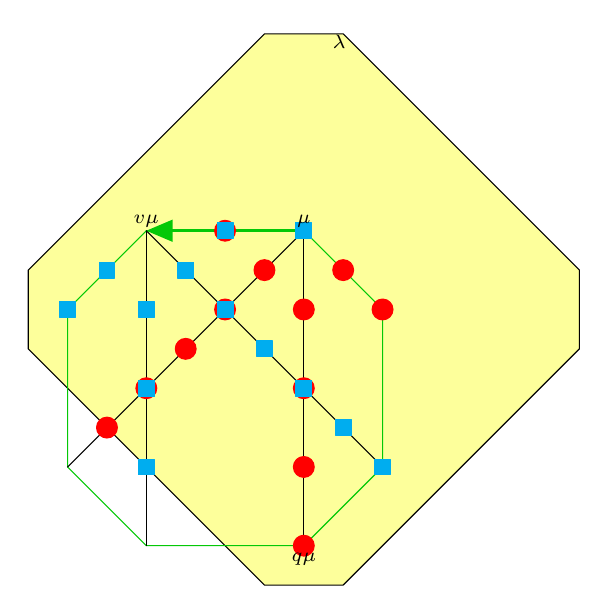
\begin{tikzpicture}[line cap=round,line join=round,>=triangle 45,x=.5cm,y=.5cm]
\draw[style=black] (1,7) -- (-1,7) -- (-7,1) -- (-7,-1) -- (-1,-7) -- (1,-7) -- (7,-1) -- (7,1) -- cycle;
\draw[style=green] (-6,-4) -- (-6,0) -- (-4,2) -- (0,2) -- (2,0) -- (2,-4) -- (0,-6) -- (-4,-6) -- cycle;
\draw (-4,2)-- (0,2);
\draw (0,2)-- (-6,-4);
\draw (0,2)-- (0,-6);
\draw  (-4,2)-- (-4,-6);
\draw  (-4,2)-- (2,-4);
\begin{scriptsize}
\draw[green, very thick, ->] (0,2) to (-4,2);
\draw (.9,6.8) node {$\lam$};
\node [style=blue] at (0,2) {};
\draw (0,2.23) node {$\mu$};
\draw (-4,2.23) node {$v\mu$};
\node [style=red] at (2,0) {};
\node [style=blue] at (2,-4) {};
\node [style=blue] at (-6,0) {};
\node [style=red] at (0,-6) {};
\draw (0,-6.35) node {$q\mu$};
\node [style=red] at (-5,-3) {};
\node [style=red] at (-4,-2) {};
\node [style=blue] at (-4,-2) {};
\node [style=blue] at (-4,-4) {};
\node [style=red] at (0,0) {};
\node [style=red] at (0,-2) {};
\node [style=red] at (0,-4) {};
\node [style=blue] at (0,-2) {};
\node [style=blue] at (-4,0) {};
\node [style=blue] at (-5,1) {};
\node [style=red] at (1,1) {};
\node [style=red] at (-2,2) {};
\node [style=blue] at (-2,2) {};
\node [style=red] at (-1,1) {};
\node [style=red] at (-2,0) {};
\node [style=blue] at (-2,0) {};
\node [style=red] at (-3,-1) {};
\node [style=blue] at (-3,1) {};
\node [style=blue] at (-1,-1) {};
\node [style=blue] at (1,-3) {};
\end{scriptsize}
\end{tikzpicture}
\caption{In this example $q\mu\leq \lam$ and the edge $\mu\raw v\mu$ is indeed swappable.}\label{figqmu<lam}
\end{center}
\end{figure}

We begin with a preliminary computation.
\begin{lemma}\label{qmuineq}
    If $q\mu\leq \lambda$ and $r\mu\not \leq \lambda$, then $-\lambda_1\leq \mu_1 \leq \lambda_1$ and $(v\mu)_2=-\mu_2-2M\leq - \lam_2$.
\end{lemma}
\begin{proof}
Observe that, since $\lam\in X_+$, for any $\nu \in X$ we have $\nu\leq \lam$ if and only if $s_1\nu\leq \lam$. So we also have $s_1r\mu=vq\mu\not\leq \lam$, $s_1q\mu =qr\mu\leq \lam$ and $s_1v \mu = vr\mu\leq \lam$. 	

If $\mu_1> \lam_1$ the line $\{ \mu - x \alpha_{21}\}_{x\in \bbR_{>0}}$ intersects the boundary of $\Conv(W\cdot \lambda)$ in the segment \[[s_2s_1\lam,s_2s_1s_2\lam]\subset H:=\{\nu \in X_\bbR \mid \langle\nu,\alpha_2^\vee\rangle= \langle s_2s_1\lam, \alpha_2^\vee\rangle=-\lam_1-\lam_2\},\] and since $r \mu \notin \operatorname{Conv}(W \cdot \lam)$ we have
	\[\langle r\mu,\alpha_2^\vee\rangle
 <-\lam_1 -\lam_2,\]
However, $qr\mu = s_1q \mu$ lies on the same side of $H$  as $r\mu$, since $\langle s_1q\mu,\alpha_2^\vee\rangle=\langle r\mu,\alpha_2^\vee\rangle$. Therefore, $s_1q\mu \not \in \Conv(W\cdot \lam)$, contradicting our assumption. Similarly, if $\mu_1<-\lam_1$, then we must have 
	\[\langle r\mu,\alpha_{12}^\vee\rangle <-\lam_1-\lam_2,\]
which implies $vr\mu=s_1v\mu \not \in\Conv(W\cdot \lam)$. We conclude theat $-\lam_1\leq \mu_1\leq \lam_1$. 

For the second part, assume that $(v\mu)_2>-\lam_2$, then 
the line $\{v\mu-x\alpha_{12}\}_{x\in \bbR_{>0}}$ intersects the segment \[[s_2s_1s_2\lam,w_0\lam]\subset H':=\{\nu \in X_\bbR \mid \langle \nu, \alpha_{21}^\vee\rangle=\langle w_0\lambda,\alpha_{21}^\vee\rangle=-\lambda_1-\lambda_2\}\] forcing
	$\langle qv\mu,\alpha_{21}^\vee\rangle<-\lam_1-\lam_2$.
	But since $\langle q\mu,\alpha_{21}^\vee\rangle=\langle qv\mu,\alpha_{21}^\vee\rangle$, this would contradict $q\mu \leq \lam$.
\end{proof}


\begin{proof}[Proof of \Cref{qmuswappable}.]

Recall that $\ell_m(\mu)=\ell_m(v\mu)-1$ by \eqref{lmX}. To conclude it is enough to show that \begin{equation}\label{elldiff}
	    \ell_m(\mu)-\ell_m(\mu,\lam) = \ell_m(v\mu)-\ell_m(v\mu,\lam)
	\end{equation} 

The proof is divided in two cases.
 Assume first that $r\mu \leq \lambda$. In this case, since additionally $q\mu \leq \lambda$, the convex hull $\Conv(W^{m+1}\cdot \mu)$ is contained in $\Conv(W\cdot \lam)$ entirely, so 
 $\ell_m(\mu,\lambda)=\ell_m(\mu)$ and $\ell_m(v\mu)=\ell_m(v\mu,\lambda)$.


We can assume now that $r\mu \not \leq \lambda$. 
By \Cref{qmuineq}, we have $-\lam_1\leq \mu_1\leq \lam_1$, which implies that $\lambda_1 + \mu_1 \geq 0$ and $\operatorname{min} (\lambda_1, \frac{\lambda_1 +\mu_1}{2}, \lambda_1 +\mu_1) = \frac{\lambda_1 +\mu_1}{2}$.
%and $(v\mu)_2\leq -\lam_2$. 
It follows from \Cref{affphicompute} that
\[ \affphi_{21}(\mu,\lam)=\mu_2+\lam_2+\frac{\mu_1+\lam_1}{2}.\]
		Since $q\mu \leq \lambda$, we have $\Arr_m^{12}(\mu)=\Arr_m^{12}(\mu,\lam)$ and \[\Arr_m^{21}(\mu)\setminus \Arr_m^{21}(\mu,\lam)=\{(\mu -k\alpha_{21})\raw \mu \mid \affphi_{21}(\mu,\lam)<k\leq \mu_1+2\mu_2+2M\},\] 
 so we get
	\begin{align}\label{Arrmu}
	\ell_m(\mu)-\ell_m(\mu,\lam) =	\ell_m^{21}(\mu)-\ell_m^{21}(\mu,\lam) =& 2M+\mu_1+2\mu_2-\affphi_{21}(\mu,\lambda)\nonumber\\
	=&2M +\mu_2 -\lam_2 +\frac{\mu_1-\lam_1}{2}.
	\end{align}
	 By \Cref{affphicompute}, since $(v\mu)_2\leq -\lam_2$ we have
	\[\affphi_{12}(v\mu,\lam)=\frac{\mu_1+\lam_1}{2}+\lam_2-M.\]
Similarly, since $rv\mu=s_1q\mu\leq \lam$ we have 
	$\Arr_m^{21}(v\mu)=\Arr_m^{21}(v\mu,\lam)$ and
	\[\Arr_m^{12}(v\mu)\setminus \Arr_m^{12}(v\mu,\lam)=\{v\mu-k\alpha_{12}\raw v\mu \mid \affphi_{12}(v\mu,\lam)<k\leq (v\mu)_1+(v\mu)_2+M\}\]
	We get
	\begin{align}\nonumber\label{arrtu}\ell_m(v\mu)-\ell_m(v\mu,\lam)&=\ell_m^{12}(v\mu)-\ell_m^{12}(v\mu,\lam)\\\nonumber&=(v\mu)_1+(v\mu)_2+M-\affphi_{12}(v\mu,\lam)\\
	&=\mu_1+\mu_2+M-\lam_2+M-\frac{\mu_1+\lam_1}{2}.\end{align}
The claimed identity \eqref{elldiff} now follows by comparing \eqref{Arrmu} and \eqref{arrtu}.
\end{proof}

As a consequence, an edge $\mu\raw v\mu$ can only be not swappable if $q\mu\not \leq \lam$. This gives some constraint on the possible location of such weights $\mu$ (see \Cref{startingpoints}).
\begin{lemma}
\label{qmuneqlambda}
	If $q\mu\not\leq \lambda$, then $\mu_1> 0$, $\mu_2<\lambda_2$ and $r\mu \not \leq \lambda$.
	%\Leo{Make explicit that there are only NS-$\alpha_2$ edges over the diagonal $\mu_1=0$.}
	%\Jaz{Done. See \Cref{mu1>0nonswap2}.}
\end{lemma}

\begin{figure}
\begin{center}
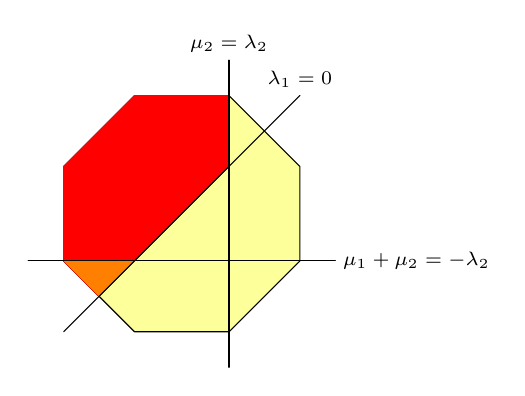
\begin{tikzpicture}[line cap=round,line join=round,>=triangle 45,x=.15cm,y=.15cm]
\draw[style=black] (4,10) -- (-4,10) -- (-10,4) -- (-10,-4) -- (-4,-10) -- (4,-10) -- (10,-4) -- (10,4) -- cycle;
\fill [red] (4,10)-- (4,4)-- (-7,-7) -- (-10,-4) -- (-10,4) -- (-4,10) -- (4,10) -- cycle;
\fill [orange]  (-4,-4)-- (-7,-7) -- (-10,-4) -- cycle;
\begin{scriptsize}
\draw (-10,-10) -- (10,10) node[above] {$\lam_1=0$}; 
\draw (4,-13) -- (4,13) node[above] {$\mu_2=\lam_2$};
\draw (-13, -4) -- (13,-4) node[right] {$\mu_1+\mu_2=-\lam_2$};    
\end{scriptsize}
\end{tikzpicture}
\end{center}
\caption{By \Cref{qmuneqlambda} the starting point of a non-swappable edge in the $\alpha_2$-direction must lie in the red or in the orange region. We further show in \Cref{mu1<lam1} that actually a starting point of a non-swappable edge can only be in the red region.}\label{startingpoints}
\end{figure}

\begin{proof}
	Assume that $q\mu \not \leq \lambda$. Then by \eqref{eqtu} and \eqref{eqqu} we have 
	\[ \affphi_2(\mu,\lambda)\geq \mu_2+M > \affphi_{12}(\mu,\lambda) -\mu_1.\]
	This is equivalent to
	\begin{equation}\label{minconfront}
		\min(\lambda_2+\mu_1+\mu_2,\lfl\frac{\lambda_2+\mu_1+\mu_2}{2}\rfl,\lambda_2)>\min(\lambda_2+\mu_2,\lfl\frac{\lambda_2+\mu_2}{2}\rfl,\lambda_2).\end{equation}
	This forces $\mu_1>0$.  Moreover, we have $\mu_2< \lambda_2$ otherwise both sides of \eqref{minconfront} would be  equal to $\lambda_2$.
	
	Notice that if $q\mu \not \leq \lam$, also $s_1q\mu\not \leq \lam$.
 Moreover,  $r=qs_1q$ and $\langle r\mu , \alpha_{12}^\vee\rangle = -\mu_2 -2M< -M$. By \eqref{bruhatorder}, we conclude that $q\mu <r\mu \not \leq \lambda$.
\end{proof}











\subsubsection{Classification of swappable edges}











%The next lemma shows that numbers of arrows pointing to $\mu$ and to $v\mu$ starting on ``the right of $\mu$'' are the same


\begin{lemma}
Assume $\mu_1\geq 0$. An edge $\mu\raw v\mu$ is swappable if and only if 
\begin{equation}\label{count1}2(\mu_2+M) +\ell_{m}^{12}(v\mu,\lambda)+\ell_{m}^{21}(v\mu,\lambda)=\ell_{m}^{12}(\mu,\lambda)+\ell_{m}^{12}(\mu,\lambda).\end{equation}
\end{lemma}
\begin{proof}
By \Cref{leqmu}, an arrow $(\mu-k\alpha_2\raw v\mu)$ is in $\Arr_m^2(\mu,\lam)$ if and only if $0\leq k< \mu_2 +M$. It follows that $\ell_m^2(\mu)=\ell_m^2(v\mu)-1$.
Moreover, by \eqref{ell1}, we have \[ \ell_{m}^{1}(\mu,\lam) = \ell_{m}^1(v\mu,\lam) - 2(\mu_2+M).\]
The claim now follows directly from \eqref{ellsubdivided}. 
\end{proof}
We now need to estimate carefully $\ell_m^{12}(\mu,\lambda)$ and $\ell_m^{21}(\mu,\lam)$, i.e., we need to characterize the arrows in $\Arr_m^{12}(\mu)$ and $\Arr_m^{21}(\mu)$ whose starting point is contained in $\Conv(W\cdot \lam)$.

%In view of \Cref{qmuswappable}, we can restrict ourselves to classify the edges $\mu \raw v\mu$ with $q\mu \not\leq \lambda$ which are swappable. We divide into two cases.

We are now ready to classify all swappable $\alpha_2$-edges. We have already seen that it is always swappable if $\mu_1\leq 0$. Now we divide the rest into two cases: $\mu_1\geq \lam_1$ and $0<\mu_1<\lam_1$.
As illustrated in \Cref{figmu1>l1}, in the case $\mu_1\geq \lam_1$ it is sufficient to compare the number of weights below $\mu$ and $v\mu$ in the convex hull of $W\cdot \lam$. We prove now this analytically. 


\begin{figure}
\begin{center}
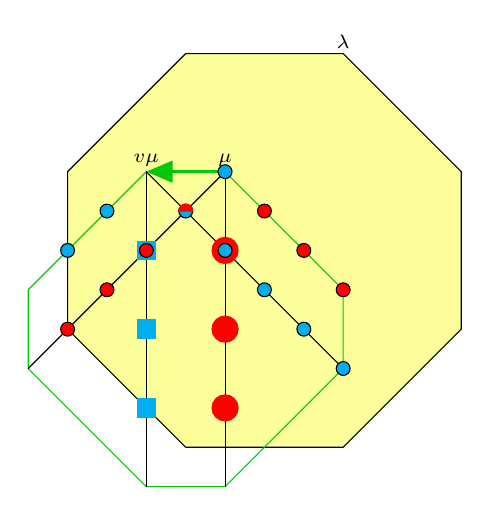
\begin{tikzpicture}[line cap=round,line join=round,>=triangle 45,x=.5cm,y=.5cm]
\draw[style =black] (2,5) -- (-2,5) -- (-5,2) -- (-5,-2) -- (-2,-5) -- (2,-5) -- (5,-2) -- (5,2) -- cycle;
\draw[style=green] (-6,-3) -- (-6,-1) -- (-3,2) -- (-1,2) -- (2,-1) -- (2,-3) -- (-1,-6) -- (-3,-6) -- cycle;
 \draw  (-1,2)-- (-6,-3);
 \draw  (-1,2)-- (-1,-6);
 \draw  (-3,2)-- (-3,-6);
 \draw  (-3,2)-- (2,-3);
 \begin{scriptsize}
\node at (2,5.3) {$\lam$};
 \node at (-1,2.3) {$\mu$};
 \node at (-3,2.3) {$v\mu$};  
 \end{scriptsize}
\draw[green, very thick, ->] (-1,2) to (-3,2);

%\draw [fill=cyan] (2,5) circle (2.5pt);
%\node[style=sblue] at (-1,2) {};
\draw [fill=cyan] (-1,2) circle (2.5pt);
%\draw [fill=cyan] (-3,2) circle (2.5pt);
\draw [fill=red] (2,-1) circle (2.5pt);
\draw [fill=cyan] (2,-3) circle (2.5pt);
\draw [fill=cyan] (-5,0) circle (2.5pt);
\draw [fill=red] (-5,-2) circle (2.5pt);
\halfcirc{-2}{1};
\draw [fill=cyan] (-4,1) circle (2.5pt);
\draw [fill=red] (0,1) circle (2.5pt);
%\draw [fill=cyan] (-2,2) circle (2.5pt);
\draw [fill=red] (-4,-1) circle (2.5pt);
\draw [fill=cyan] (0,-1) circle (2.5pt);
\draw [fill=cyan] (1,-2) circle (2.5pt);
\draw [fill=red] (1,0) circle (2.5pt);

\node[style=red] at (-1,-2) {};
\node[style=red] at (-1,-4) {};
\node[style=red] at (-1,0) {};
\node[style=blue] at (-3,-2) {};
\node[style=blue] at (-3,-4) {};
\node[style=blue] at (-3,0) {};
\draw [fill=red] (-3,0) circle (2.5pt);
\draw [fill=cyan] (-1,0) circle (2.5pt);
\end{tikzpicture}
\end{center}
\caption{We have $\mu_1\geq \lam_1$, so to check whether $\mu\raw v\mu$ is swappable we just need to count the weights below $\mu$ and $v\mu$. In this example they are both $3$, hence the edge is swappable.}\label{figmu1>l1}
\end{figure}


\begin{proposition}\label{mu1geqlam1}
Let $\mu$ be such that $\mu_1\geq \lam_1$. Then $\mu\raw v\mu$ is swappable if and only if 
\[ \mu_2\geq -\lam_2+1\text{ and }M \leq \lce \frac{\lam_2-\mu_2 }{2}\rce.\]
\end{proposition}
\begin{proof}


Since $\mu_1\geq \lam_1$ and $\mu\leq \lam$, we have $\mu_2\leq \lam_2$.
	Since $\mu <v\mu$ we have $M+\mu_2 >0$.
We know that if $q\mu \leq \lam$ then $\mu \raw v\mu $ is swappable. In the other direction, if $\mu_2\leq -\lam_2$ or $\mu_2>-\lam_2$ and $M> \lce \frac{\lam_2-\mu_2 }{2}\rce$ then it follows from \eqref{eqqu} that $q\mu\not \leq \lam$. So it is enough to consider the case $q\mu \not \leq \lam$.

We have $\lam_1\leq \mu_1< (v\mu)_1$ and $(v\mu)_2\leq \lam_2$. In this case, we have 
\begin{equation}\label{phi12vu} \affphi_{21}(v\mu,\lambda)=\lam_1 + \lam_2 -\mu_2 -2M = \affphi_{21}(\mu,\lambda)-2(\mu_2+M).
\end{equation}

Combining this with \eqref{count1} and \eqref{eqqu} we get that $\mu\raw v\mu$ is swappable if and only if 
$\affphi_{12}(\mu,\lambda)=\affphi_{12}(v\mu,\lambda)$, which is equivalent to
\[ \min \left(\lam_2+\mu_2,\lfl \frac{ \lam_2+ \mu_2}{2}\rfl\right)=\min\left(\lam_2-M ,\lfl \frac{ \lam_2+ \mu_2}{2}\rfl\right).\]
This equality holds if and only if both minima are achieved at  $\lfl \frac{ \lam_2+ \mu_2}{2}\rfl$, i.e. if
\[ \lam_2 + \mu_2 \geq \lfl \frac{ \lam_2+ \mu_2}{2}\rfl\leq \lam_2 -M.\]
So we have $-\mu_2< M\leq \lce \frac{\lam_2-\mu_2 }{2}\rce$, which is equivalent to $\mu_2\geq -\lam_2+1$ and the claim follows.
\end{proof}

% \begin{proposition}
% \label{mu1<lam1}
% 	Let $\mu\leq \lam$ be such that $0<\mu_1< \lam_1$. Then $\mu\raw v\mu\in E^N(\lam)$ if and only if the following conditions hold
% \begin{equation}\label{mu1>lam1ineq}\mu_2\geq -\lam_2+1\quad\text{and}\quad
% M>\frac{\lam_1-\mu_1}{2}+\lce\frac{\lam_2-\mu_2}{2} \rce.\end{equation}
% \end{proposition}
% \begin{proof}
% Notice that if the the two inequalities in \eqref{mu1>lam1ineq}, then $q\mu\not \leq \lam$ by \eqref{eqqu}. Since $\mu\raw v\mu$ is swappable if $q\mu\leq \lam$, we can just assume that $q\mu\not \leq \lam$.

% We begin by proving the following inequality.
% \begin{claim}\label{claimtmu}
%  We have $(v\mu)_2< -\lam_2$.
% \end{claim}
% \begin{proof}[Proof of the claim.]
% We have $(v\mu)_2=-\mu_2-2M$.
% If $\mu_2\leq -\lam_2$, then $-\mu_2-2M<-M<\mu_2\leq -\lam_2$. If $\mu_2\geq \lam_2$, we have $-\mu_2-2M<-\mu_2\leq -\lam_2$.

% If $-\lam_2<\mu_2<\lam_2$, then we have by \eqref{eqqu} that
% \begin{align*} -\mu_2-2M&<\mu_2+2\mu_1-2\affphi_{12}(\mu,\lam)\\
% &=-\lam_1+\mu_1+\mu_2-2\lfl\frac{\lambda_2+\mu_2}{2}\rfl\leq -\lam_2\qedhere
% \end{align*}
% \end{proof}



% Assume first $\mu_1<(v\mu)_1\leq \lam_1$, or equivalently that $M \leq \frac{\lam_1-\mu_1}{2}-\mu_2$. Since $q\mu \not \leq \lambda$, we have by \eqref{eqqu} that
% \begin{equation}\label{notsmaller}M>\frac{\lam_1-\mu_1}{2}-\min(\lam_2,\lfl \frac{\lam_2-\mu_2}{2}\rfl),\end{equation}
% forcing $\mu_2<M-\frac{\lam_1-\mu_1}{2}<-\lam_2$. Now we can easily compute both sides of \eqref{count1} 
% and check that they are both equal to $\lam_1+\mu_1+2(\lam_2+\mu_2)$. So $\mu\raw v\mu$ is always swappable.


% Assume now $\mu_1<\lam_1<(v\mu)_1$, that is, that $M>\frac{\lam_1-\mu_1}{2}-\mu_2$. Since we assumed that $q\mu \not\leq \lam$, by \eqref{eqqu}, we also have  that 
% \begin{equation}\label{notsmaller2}M>\frac{\lam_1-\mu_1}{2}+\lfl\frac{\lam_2-\mu_2}{2}\rfl.\end{equation}

% In this case \eqref{count1} is equivalent to 
% \begin{equation}\label{mu1<lam1eq} \frac{3\lam_1+\mu_1}{2}+2\lam_2+\mu_2-M= \lam_1+\mu_1+\lam_2+\mu_2+\min\left(\lam_2+\mu_2,\lfl \frac{\lam_2+ \mu_2}{2}\rfl\right)\end{equation}
% and we get an equality if and only if %\[M=\max(\mu_2,\frac{\lam_2+\mu_2}{2},0)-\min(\lambda_1,\lfl \frac{\lambda_1+\mu_1}{2}\rfl)\]
% \[M = \frac{\lam_1-\mu_1}{2}+\max\left(-\mu_2,\lce\frac{\lam_2-\mu_2}{2}\rce\right)\] 
% However, since  $M>\frac{\lam_1-\mu_1}{2}-\mu_2$, we must have 
% $-\mu_2 < \lce \frac{\lam_2-\mu_2}{2}\rce$, which is equivalent to $\mu_2\geq -\lam_2+1$, and $M= \frac{\lam_1-\mu_1}{2}+\lce\frac{\lam_2-\mu_2}{2}\rce$.
% Notice that by \eqref{notsmaller2} we cannot have $M< \frac{\lam_1-\mu_1}{2}+\lce\frac{\lam_2-\mu_2}{2}\rce$. The claim now follows.




% %\[ M > \frac{\lambda_1-\mu_1}{2}+\min(\lam_2,\lfl\frac{\lam_2-\mu_2}{2}\rfl)\]
% %which implies
% %\[\min(\lam_2,\lfl\frac{\lam_2-\mu_2}{2}\rfl)< \max(-\mu_2,\lce\frac{\lam_2-\mu_2}{2}\rce),\]
% %
% %If $\mu_2\equiv \lam_2 \pmod{2}$, this implies $\mu_2<-\lam_2$. So, we have
% %\[ M = \frac{\lam_1-\mu_1}{2}-\mu_2\]
% %and $(v\mu)_1= \lam_1$, which is a contradiction, so $\mu \raw v\mu$ is not swappable.
% %
% %If $\mu_2\not\equiv \lam_2 \pmod{2}$, then there is an extra possibility:
% %\[ M = \frac{\lam_1-\mu_1}{2}-\lfl\frac{\mu_2-\lam_2}{2}\rfl\]
% \end{proof}
\begin{proposition}
\label{mu1<lam1}
	Let $\mu\leq \lam$ be such that $0<\mu_1< \lam_1$. Then $\mu\raw v\mu\in E^N(\lam)$ if and only if
\begin{equation}\label{mu1>lam1ineq}
M>\frac{\lam_1-\mu_1}{2}+\max\left(-\mu_2,\lce\frac{\lam_2-\mu_2}{2} \rce\right).\end{equation}
\end{proposition}
\begin{proof}
Notice that if the inequality \eqref{mu1>lam1ineq} holds, then $q\mu\not \leq \lam$ by \eqref{eqqu}. Since $\mu\raw v\mu$ is swappable if $q\mu\leq \lam$, we can just assume that $q\mu\not \leq \lam$.

We begin by proving the following inequality.
\begin{claim}\label{claimtmu}
 We have $(v\mu)_2< -\lam_2$.
\end{claim}
\begin{proof}[Proof of the claim.]
We have $(v\mu)_2=-\mu_2-2M$.
If $\mu_2\leq -\lam_2$, then $-\mu_2-2M<-M<\mu_2\leq -\lam_2$. If $\mu_2\geq \lam_2$, we have $-\mu_2-2M<-\mu_2\leq -\lam_2$.

If $-\lam_2<\mu_2<\lam_2$, then we have by \eqref{eqqu} that
\begin{align*} -\mu_2-2M&<\mu_2+2\mu_1-2\affphi_{12}(\mu,\lam)\\
&=-\lam_1+\mu_1+\mu_2-2\lfl\frac{\lambda_2+\mu_2}{2}\rfl\leq -\lam_2\qedhere
\end{align*}
\end{proof}



Assume first $\mu_1<(v\mu)_1\leq \lam_1$, or equivalently that $M \leq \frac{\lam_1-\mu_1}{2}-\mu_2$. Since $q\mu \not \leq \lambda$, we have by \eqref{eqqu} that
\begin{equation}\label{notsmaller}M>\frac{\lam_1-\mu_1}{2}-\min(\lam_2,\lfl \frac{\lam_2-\mu_2}{2}\rfl),\end{equation}
forcing $\mu_2<M-\frac{\lam_1-\mu_1}{2}<-\lam_2$. Now we can easily compute both sides of \eqref{count1} 
and check that they are both equal to $\lam_1+\mu_1+2(\lam_2+\mu_2)$. So $\mu\raw v\mu$ is always swappable.


Assume now $\mu_1<\lam_1<(v\mu)_1$, that is, that $M>\frac{\lam_1-\mu_1}{2}-\mu_2$. Since we assumed that $q\mu \not\leq \lam$, by \eqref{eqqu}, we also have  that 
\begin{equation}\label{notsmaller2}M>\frac{\lam_1-\mu_1}{2}+\lfl\frac{\lam_2-\mu_2}{2}\rfl.\end{equation}

In this case \eqref{count1} is equivalent to 
\begin{equation}\label{mu1<lam1eq} \frac{3\lam_1+\mu_1}{2}+2\lam_2+\mu_2-M= \lam_1+\mu_1+\lam_2+\mu_2+\min\left(\lam_2+\mu_2,\lfl \frac{\lam_2+ \mu_2}{2}\rfl\right)\end{equation}
and we get an equality if and only if %\[M=\max(\mu_2,\frac{\lam_2+\mu_2}{2},0)-\min(\lambda_1,\lfl \frac{\lambda_1+\mu_1}{2}\rfl)\]
\begin{equation}\label{Mlimit}
    M = \frac{\lam_1-\mu_1}{2}+\max\left(-\mu_2,\lce\frac{\lam_2-\mu_2}{2}\rce\right)
\end{equation}
%However, since  $M>\frac{\lam_1-\mu_1}{2}-\mu_2$, we must have $-\mu_2 < \lce \frac{\lam_2-\mu_2}{2}\rce$, which is equivalent to $\mu_2\geq -\lam_2+1$, and $M= \frac{\lam_1-\mu_1}{2}+\lce\frac{\lam_2-\mu_2}{2}\rce$.
Notice that by \eqref{notsmaller2} we cannot have $M< \frac{\lam_1-\mu_1}{2}+\lce\frac{\lam_2-\mu_2}{2}\rce$. The claim now follows.
\end{proof}

We can restate \Cref{mu1<lam1} in more convenient terms.

\begin{corollary}
    Assume $0<\mu_1<\lam_1$. Then $(\mu \raw v \mu)\in E^N(\lam)$ if and only if $\lam_1<(v\mu)_1$ and $q\mu\not \leq \lam$, except when $\lam_2 \not \equiv \mu_2 \pmod{2}$, $\lam_2+\mu_2>0$ and
    \[ M = \frac{\lam_1-\mu_1}{2}+\frc{\lam_2-\mu_2}\]
\end{corollary}
\begin{proof}
As in the proof of \Cref{mu1<lam1}, we know that the only case in which $\lam_1<(v\mu)_1$, $q\mu \not \leq \lam$ and $(\mu \raw v\mu)\in E^S(\lam)$ is for $M$ as in \eqref{Mlimit}.
    Since $\lam_1<(v\mu)_1$ then $M>\frac{\lam_1-\mu_1}{2}-\mu_2$. Since $q\mu\not \leq \lam$ then $M>\frac{\lam_1-\mu_1}{2}+\frc{\lam_2-\mu_2}$.
So the equality in \eqref{Mlimit} is possible if and only if 
$\frc{\lam_2-\mu_2}>\frf{\lam_2-\mu_2}$ and $\frc{\lam_2-\mu_2}>-\mu_2$, i.e. if $\lam_2 \not \equiv \mu_2\pmod{2}$ and $\lam_2+\mu_2\geq1$.   
\end{proof}

\begin{example}
Let $\lam=(3,2)$, $\mu=(1,-1)$ and $M=\frac{\lam_1-\mu_1}{2}-\frc{\lam_2-\mu_2}=3$. As illustrated in \Cref{limitcase}, in this case the edge $\mu\raw v\mu$ is swappable even if $(v\mu)_1>\lam_1$.
\end{example}

\begin{figure}
\begin{center}
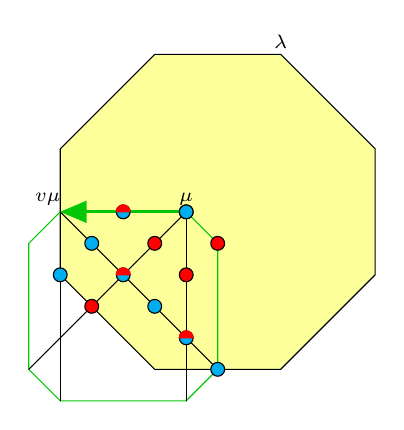
\begin{tikzpicture}[line cap=round,line join=round,>=triangle 45,x=.4cm,y=.4cm]
\draw[style=black] (2,5) -- (-2,5) -- (-5,2) -- (-5,-2) -- (-2,-5) -- (2,-5) -- (5,-2) -- (5,2) -- cycle;
\draw[style=green] (-6,-5) -- (-6,-1) -- (-5,0) -- (-1,0) -- (0,-1) -- (0,-5) -- (-1,-6) -- (-5,-6) -- cycle;
\draw  (-1,0)-- (-6,-5);
\draw  (-1,0)-- (-1,-6);
\draw  (-5,0)-- (-5,-6);
\draw  (-5,0)-- (0,-5);
\begin{scriptsize}
\draw [fill=cyan] (-1,0) circle (2.5pt);
\draw [fill=red] (0,-1) circle (2.5pt);
\draw [fill=red] (-4,-3) circle (2.5pt);
\draw [fill=red] (-1,-2) circle (2.5pt);
\draw [fill=cyan] (-5,-2) circle (2.5pt);
\draw[green, very thick, ->] (-1,0) to (-5,0);

\halfcirc{-3}{0}
\halfcirc{-3}{-2}
\halfcirc{-1}{-4}
\node at (2,5.4) {$\lam$};
\node at (-1,0.4) {$\mu$};
\node at( -5.4,0.4) {$v\mu$};

\draw [fill=red] (-2,-1) circle (2.5pt);
\draw [fill=cyan] (-4,-1) circle (2.5pt);
\draw [fill=cyan] (-2,-3) circle (2.5pt);
\draw [fill=cyan] (-1,0) circle (2.5pt);
\draw [fill=cyan] (0,-5) circle (2.5pt);
\end{scriptsize}
\end{tikzpicture}
\end{center}
\caption{The exceptional case in which the edge $\mu\raw v\mu$ is swappable even if $(v\mu)_1>\lam_1$.}
\label{limitcase}
\end{figure}


\subsection{Analysis of \texorpdfstring{$\alpha_{12}$-}{vertical }edges}

Assume now that $m+1=4M-2$, so that $q_M:=t_{m+1}$ is the reflection corresponding to the root $M\delta-\alpha_{12}^\vee$, i.e. a reflection over the hyperplane $\{\nu \mid \langle \nu,\alpha_{12}^\vee\rangle =-M\}$. Let $r:=r_M$, $q:=q_M$ and $v:=v_M$ so that the reflections in the reflection subgroup $W^{m+1}$ are $\{s_1,r,q,v\}$. The classificiation of NS-edges in the $\alpha_{12}$-direction can be reduced to the known case of $\alpha_2$-edges, as the \Cref{12notswap} shows.

\begin{proposition}\label{12notswap}
An edge of the form $\mu \ra q\mu$ is swappable if and only if $s_1\mu\ra v s_1\mu$ is swappable.
\end{proposition}
\begin{proof}
It is enough to show that
\begin{equation}\label{ellm+2} \ell_m(\mu,\lam)-\ell_m(q\mu,\lam)=\ell_{m+2}(s_1\mu,\lam)-\ell_{m+2}(vs_1\mu,\lam).
\end{equation}


\begin{claim}
Conjugation by $s_1$ induces a  bijection \[\Arr_m(\mu,\lambda)\setminus \{s_1\mu\raw \mu\}\cong \Arr_m(s_1\mu,\lam)\setminus \{\mu \raw s_1\mu\}\] which sends $(u\mu \raw \mu)$ to $(s_1 u \mu \raw s_1 \mu)$. In particular, we have  $\ell_m(\mu,\lam)=\ell_m(s_1\mu,\lam)+1$ if $\mu_1>0$.
\end{claim}
\begin{proof}[Proof of the claim.]
Notice that, since $m=4M-3$, we have  $\beta^\vee\in N(y_m)$ if and only if $s_1(\beta^\vee)\in N(y_m)$.
If $t\mu<_m\mu$ for $t=s_{N\delta-\alpha^\vee}$ with $\alpha^\vee\in \{\alpha_2^\vee,\alpha_{12}^\vee,\alpha_{21}^\vee\}$, then also $s_1(\alpha^\vee)\in \{\alpha_2^\vee,\alpha_{12}^\vee,\alpha_{21}^\vee\}$
and, since $\langle \mu,\alpha^\vee\rangle = \langle s_1(\mu),s_1(\alpha^\vee)\rangle$ it follows by \eqref{bruhatorder} that also $s_1 t s_1s_1(\mu) <_m s_1(\mu)$.
If $t=s_{N\delta+\alpha_1^\vee}$ with $N\neq 0$, then $s_1ts_1=s_{N\delta-\alpha_1^\vee}$
and we have
\begin{align*}
    t\mu <_m \mu &\iff \sgn(N) \langle \mu, \alpha_1^\vee\rangle >|N|\\
    & \iff \sgn(-N) \langle s_1(\mu), \alpha_1^\vee\rangle>|-N|\\
    & \iff s_1t(\mu)<_m s_1(\mu).\qedhere
\end{align*} 
\end{proof}

We assume now $\mu_1< 0$ and let $\nu=s_1(\mu)$. Notice that $(q\mu)_1<0$.
Since $vs_1=s_1q$, using the claim, \eqref{ellm+2} is equivalent to
\[\ell_m(\nu,\lam)-\ell_m(v\nu,\lam)=\ell_{m+2}(\nu,\lam)-\ell_{m+2}(v\nu,\lam).\]


For any weight $\mu'$, 
the symmetric difference $\Arr_m(\mu',\lam)\vartriangle \Arr_{m+2}(\mu',\lam)$ is contained in $\{q\mu'\raw \mu', r\mu'\raw \mu'\}$ since these are the two only edges which we are possibly reversing. Then the claim follows since we have 
\[ \ell_{m+2}(\nu,\lam)-\ell_m(\nu,\lam) = |\{q\nu,r\nu\} \cap \{\leq \lam\}|= \ell_{m+2}(v\nu,\lam)-\ell_m(v\nu,\lam).\]
In fact, by \Cref{bruhatorderWk} we have $\nu<q\nu$, and $v\nu<rv\nu$ and $qv\leq \lam \iff s_1q\nu =rv\nu<\lam$. Similarly, we have $\nu<r\nu$ and $v\nu <qv\nu$ and $r\nu \leq \lam \iff s_1r\nu =qr\nu < \lam$.

The case $\mu_1\geq 0$ is similar.
\end{proof}




\subsection{Analysis of \texorpdfstring{$\alpha_{21}$-}{diagonal }edges}

We conclude the classification of swappable edges by looking at edges in the $\alpha_{21}$-direction. In this case, the classification is trivial since, as it turns out, all the $\alpha_{21}$-edges are swappable. 
% Assume now that $t_{m+1}$ is the reflection corresponding to the root $M\delta-\alpha_{21}^\vee$, i.e. a reflection over the hyperplane $\{\nu \mid \langle \nu,\alpha_{21}^\vee\rangle =-M\}$. In this case, $m+1$ is odd. The reflections in the reflection subgroup $W^{m+1}$ are
% $\{s_1,r,q,t\}$ where $q=s_{M/2\delta-\alpha_{12}^\vee}$ and $t=s_{M/2\delta-\alpha_{2}^\vee}$
\begin{proposition}
\label{21swappable}
Any edge of the form $\mu \ra \mu-k\alpha_{21}$ is swappable.
\end{proposition}
\begin{proof}
We can assume that $\mu-k\alpha_{21}=s_{(2M-j)\delta -\alpha_{21}^\vee}(\mu)$ with $j=0$ or $j=1$. The root $(2M-j)\delta -\alpha_{21}^\vee$ is the $(4M-1-2j)$-th root occurring in \eqref{reflectionorder}.  Let $m+1=4M-1-2j$ so that $r:=t_{m+1}=s_{(2M-j)\delta -\alpha_{21}^\vee}$.

We have $\ell^1(\mu)=\ell^1(r\mu)$ and $\ell^{21}(\mu,\lam)=\ell^{21}(r\mu,\lam)-1$, so to show that $\mu\raw r\mu$ is swappable it is enough to check that
\begin{equation}\label{ell212}
  \ell^2(\mu,\lam)+\ell^{12}(\mu,\lam)=\ell^2(r\mu,\lam)+\ell^{12}(r\mu,\lam).  
\end{equation} 
 

We consider first the case $j=0$, so $W^m$ is the reflection subgroup with reflections $s_1,q_M,r_M,v_M$. Notice that $r=r_M$.
If $\mu_1\geq 0$ and $v_M\mu \geq\mu$ then
 $\Conv(W^m\cdot \mu)\subset \Conv(W\cdot \lam)$ and the edge $\mu \ra r\mu$ is swappable by the same argument as in the proof of \Cref{qmuswappable}.
 
 Assume now $\mu_1\geq 0$ and $v_M\mu < \mu$.
 Notice that we also have $v_Mr\mu < r\mu$.
 If $q\mu \leq \lam$, then again $\Conv(W^m\cdot \mu)\subset \Conv(W\cdot \lam)$. If $q\mu \not \leq \lam$, then also $s_1q\mu =qr\mu\not \leq \lam$ and we can rewrite \eqref{ell212} as
 \begin{equation}\label{diagonalcount} \ell^2_m(\mu)+\affphi_{12}(\mu,\lam)=\ell^2_m(r\mu)+\affphi_{12}(r\mu,\lam).\end{equation}

\begin{claim}
    We have $\mu_2<-\lam_2$.
\end{claim}
\begin{proof}[Proof of the claim.]
we have $\mu>v_M\mu$ so $\mu_2+M<0$. If $\mu_2\geq -\lam_2$ then $\affphi_{12}(\mu,\lam)=\lam_1+\mu_1+\frf{\lam_2+\mu_2}$ and $q\mu\not\leq \lam$ implies by \eqref{eqqu} that $\mu_1+\mu_2+2M>\lam_1+\lam_2$.  In particular, $\mu_1> \lam_1+\lam_2-\mu_2-2M\geq \lam_1$, so $\affphi_{21}(\mu,\lam)=\lam_2+\mu_2+\lam_1$ but this leads to a contradiction since $r\mu\leq \lam$ and by \eqref{eqru} we get $\mu_1+\mu_2+2M\leq\lam_1+\lam_2$.
\end{proof}

We now go back to the proof of \eqref{diagonalcount}.
 We have $\ell^2_m(\mu)=-\mu_2-M-1$ and $\ell^2_m(r\mu)=\mu_1+\mu_2+M-1$. Since $\mu_2<-\lam_2$ we have by \Cref{affphicompute} that $\affphi_{12}(\mu,\lam)=\frac{\mu_1+\lam_1}{2}+\lam_2+\mu_2$ and $\affphi_{12}(r\mu,\lam)=\frac{\mu_1+\lam_1}{2}+\lam_2-\mu_1-\mu_2-2M$ and the claim easily follows. The case $\mu_1<0$ is analogous.



 Consider now the case $j=1$. The proof here is similar, with the main difference being that the reflections in  $W^m$ are $s_1,q_M,r_M,v_M$ but $r\neq r_M$. In fact, we  have  $r=s_{(2M-1)\delta-\alpha_{21}^\vee}$ and $r_M=s_{2M\delta-\alpha_{21}^\vee}$. In the case $\mu_1\geq 0$ and $v_M\mu\geq \mu$, or $q_M\mu\leq \lam$ then,  similarly to the previous case, we have
 \[ \{\leq_m \mu\} \subset \Conv(W^m\cdot \mu)\setminus \{r_M\mu\} \subset \Conv(W\cdot \lambda).\]
 (In other words, the convex hull of $W^m\cdot \mu$ must lie inside $\Conv(W\cdot \lam)$, except possibly for $r_M\mu$, but this does not matter since $\mu <_m r_M\mu$.)
 It follows that $\mu \raw r\mu$ is swappable. If $\mu>v_M\mu$ and $q_M\mu \not \leq \lambda$ then we conclude by checking the identity \eqref{diagonalcount} as before. The case $\mu_1<0$ is symmetric.
\end{proof}




\subsection{Consequences of the classification}

We can summarize the results from the previous in three sections in the following proposition.


\begin{proposition}
    \label{mu1>0nonswap2}
Assume $\mu_{1} >0$ and let $t$ be a reflection. If the edge $\mu \ra t\mu$ is not swappable, then $t$ corresponds to a root of the form $M\delta -\alpha^{\vee}_{2}$. 
\end{proposition}

\begin{proof}
By \Cref{21swappable}, we know that $\mu \ra t_{m+1}\mu$ cannot be in the $\alpha_{21}$-direction. Since $\mu_1\geq 0$, by \Cref{12notswap} we also know that it cannot be in the $\alpha_{12}$-direction. Hence, the only possibility is that it is an edge in the $\alpha_2$ direction.
\end{proof}

The classification of swappable edges also allows us to easily compare swappable edges for different atoms.

\begin{proposition}\label{corcon}
Let $\mu \leq \lam$ with $\mu_1\geq 0$. Let $m=4M$ so that $t_m=s_{M\delta-\alpha_2^\vee}$ and assume $\mu <t_m\mu \leq \lambda$. Consider the arrow $(\mu\raw t_m\mu)\in E(\lam)$.
\begin{enumerate}
    \item \label{smallerbad}
If $(\mu\raw t_m\mu)\in E^S(\lambda)$, then $(\mu\raw t_m\mu)\in E^S(\lambda+k\varpi_2)$, for any $k\geq 0$.
 \item If $(\mu\raw t_m\mu)\in E^S(\lambda)$, then  for any $k<m$ such that $\mu<t_k\mu\leq \lam$, we also have $(\mu\raw t_k\mu)\in E^S(\lam)$. 
 \item If $(\mu\raw t_m\mu)\in E^N(\lambda)$, then $\lambda - \varpi_2$ is dominant and $\mu\leq \lambda-\varpi_2$.
\end{enumerate}
\end{proposition}
\begin{proof}
The first two statements are clear from the explicit description given in \Cref{mu1geqlam1} and \Cref{mu1<lam1}.
%\Jaz{In the proof of 1., how do you show $\mu_2 < -\lambda_2 +k -1 = -(\lambda_2+k) +1$ for $< \mu_1 < \lam_1$? In \Cref{mu1<lam1} the condition is for non-swaps so we need to turn it around.}\Leo{Yeah, good point... The condition in \Cref{mu1<lam1} is wrong. I think it should be just $M > \frac{\lam_1-\mu_1}{2}+\max\left(-\mu_2,\lce\frac{\lam_2-\mu_2}{2}\rce\right)$. I hope this does not change too many proofs.} \\
%\Leo{Proof of the third one?}

To prove $3.$ first notice that if $\lambda_2 = 0$, by \Cref{qmuneqlambda} and \Cref{mu1<lam1} there can be no non-swappable edges. 


\
\
\


We now need to show the inequalities from Lemma \ref{octineq} for $\mu$ and for $\lam' = \lam - \varpi_{2}$. In fact, by \Cref{qmuneqlambda} and \Cref{mu1<lam1}, we only need to establish the following inequalities, since they describe the hyperplanes delimiting the red region in \Cref{startingpoints}:

\begin{enumerate}
\item \label{3.1} $\mu_1 + \mu_2 \leq \lambda_1 + \lambda_2 -1$
\item \label{3.2} $\mu_1 \leq \lambda_1 + 2\lambda_2 - 2$
\item \label{3.3} $\mu_2 \geq -\lambda_1 - \lambda_2 +1$
\end{enumerate}

However note that if $\mu$ lies on either one of the hyperplanes defined by $\mu_1 = \lambda_1 + 2\lambda_2$ or $\mu_2 = -\lambda_1 -\lambda_2 $ or , then $t_m \mu \nleq \lambda$ since $t_m\mu$ is ``on the left'' of $\mu$. Therefore the only inequality we really need to prove is \ref{3.1}.

We assume that the inequality is not true, that is, $\mu$ lies in the hyperplane defined by $\lambda_1 +\lambda_2 = \mu_1 +\mu_2$. In particular, since $\mu \leq \lambda$, such $\mu$ must belong to the ``top side'' of the octagon $\Conv(W\cdot \lam)$ and it must satisfy $\lambda_1 \leq \mu_1 \leq \lambda_1 + 2\lambda_2$ and $-\lam_2\leq \mu_2\leq 
\lam_2$. Also $(t_m\mu)_2$ must lie on the same side of the octagon, so  necessarily then $(t_m \mu)_2 = -\mu_2 -2M \geq -\lambda_2$, which holds if and only if 
\[ M \leq \frac{\lambda_2 -\mu_2}{2}.\]
We get a contradiction, since by  \Cref{mu1geqlam1} the edge $\mu\raw t_m\mu$ is swappable.

% \noindent Therefore since our edge is non-swappable, \Cref{mu1geqlam1} implies that \[\mu_2 < -\lambda_2 +1,\] which is impossible since we assumed $\mu_2 >0$. However if $\mu_2 \leq 0$ we also get a contradiction, since in that case we have by the previous reasoning also  $\mu_2 < -\lambda_2 +1$, however $\mu_2 \geq -\lambda_2$ since $\mu \leq \lambda$. This would imply that $\mu_2 = -\lambda_1$, but then $t_m \mu \nleq \lambda$, a contradiction. 







%We also need to prove that $\lambda'$ is dominant, or, equivalently, $\lambda_2 >0$. Our conditions imply that $\mu_{2} \leq -M < 0$, and by \Cref{mu1<lam1remark} we have $\lambda_2 + \mu_2 >1$. Putting both together we deduce that certainly $\lambda_2 >0$. 

%By (\ref{supp4}) in the proof of  \Cref{smallerissmaller}, we have $\mu_1 \leq \lam_1 +2\lam_2 -2M \leq \lam_1 +2\lam_2 -2$. The inequality $-\lam_1 - 2\lam_2 \leq \mu_1$ is trivial because by assumption $\mu_1 \geq 0$ and $\lambda$ is dominant. This proves the first inequality from Lemma \ref{octineq} for $\mu \leq \lam - \varpi_2$.

%Since $\lambda$ is dominant and by Proposition $\mu_2 \geq -\lambda_{2} + 1$ we have $-\lambda_1 -\lambda_2 -1 \leq -\lambda_2 -1 \leq \mu_2.$ The inequality $\mu_2 \leq \lambda_1 +\lambda_2 -1$ follows from the assumption that $\mu \leq t_m \mu$ which implies that $\mu \leq -M$, in particular $\mu_2 \leq -1$. This proves the third inequality from Lemma \ref{octineq} for $\mu \leq \lam - \varpi_2$.

%The condition $t_m \mu \leq \lambda$ implies by (\ref{bruhatorder}) that $\mu_1 +2\mu_2 +2M \leq \lambda_1 +2\lambda_2$. Since $M \geq 1$ this implies $\mu_1 + 2\mu_2 \leq \lambda_1 +2\lambda_2 -2$. The inequality $\mu_2 \geq -\lambda_2 +1$ combined with the second inequality from Lemma \ref{octineq} for $\mu \leq \lam$ implies $\mu_1 +2\mu_2 \geq -\lam_1 -\lam_2 -\lam_2 +1$. This proves the fourth inequality from Lemma \ref{octineq} for $\mu \leq \lam - \varpi_2$. 

%If $0 < \mu_1 < \lambda_1$, the inequality $-\lambda_1-\lambda_2 + 1 \leq \mu_1 +\mu_2$ follows directly from  \Cref{mu1<lam1remark} since then $\mu_2 \geq -\lambda_2 +1$. Moreover, we have 
%$1 \leq 2M \leq \lambda_1 +\lambda_2 -(\mu_1+\mu_2)$, which implies $\mu_1 +\mu_2 \leq \lambda_1 +\lambda_2 -1$. If $\mu_{1}\geq \lambda_1$, the inequality $\mu_1 + \mu_2 \leq \lambda_1 +\lambda_2 $ it follows from \Cref{mu1geqlam1} which implies $\mu_2 < -\lambda_2 +1$ combined with the inequality $\mu \leq \lambda_1 +2\lambda_2 -2$ which comes from the first inequality for $\mu \leq \lambda - \varpi_2$. The inequality $-\lambda_1 -\lambda_2 +1 \leq \mu_1 +\mu_2$ is a result of combining the inequality $-\mu_2> \lambda_2 - 1$ and $-\lam_1 -2\lam_2+2 \leq \mu_1 + 2\mu_2$ coming from the fourth inequality for $\mu \leq \lam -\varpi_2$. This proves the second inequality from Lemma \ref{octineq} for $\mu \leq \lam - \varpi_2$.
\end{proof}




We are now ready to count the number of non-swappable edges.


\begin{definition}
\label{nonswappablenumber}
	For $\mu\leq \lambda$ and $m\in \bbN$, we denote by
% 		\[\calS(\mu,\lambda):=|\{ k \in \bbZ \mid  \mu<t_k\mu \leq \lambda \text{ and }\mu\raw t_k\mu\text{ is swappable}\}|\]
	\[\calN_m(\mu,\lambda):=|\{k \leq m \mid  \mu<t_k\mu \leq \lambda \text{ and }\mu\raw t_k\mu\text{ is not swappable}\}|\]
	the number of  non-swappable edges in $E^N(\lambda)$ corresponding to a reflection $t_k$, for $k\leq m$, with starting point $\mu$. Let
\
\[\calN_\infty(\mu,\lam):=\left\lvert\{k \in \bbN \mid  \mu<t_k\mu \leq \lambda \text{ and }\mu\raw t_k\mu\text{ is not swappable}\}\right\rvert.\]
\end{definition}	

\begin{lemma}\label{Nintmuis0}
If $\mu\leq t_m\mu\leq \lam$, then $\calN_m(t_m\mu,\lam)=0$.
\end{lemma}
\begin{proof}
If $(t_m\mu)_1\geq 0$, this follows directly from \Cref{smallerissmaller}. The case $(t_m\mu)<0$ is symmetric.
% If $(t_m\mu)_0> 0$, then only $\alpha_2$-edges can be non-swappable. If $t_m=s_{M\delta-\alpha_2^\vee}$,
% then $\calN_m(t_{m+1}\mu,\lam)=0$ because $s_{K\delta-\alpha_2^\vee}s_{M\delta-\alpha_2^\vee}\mu<s_{M\delta-\alpha_2^\vee}\mu$ for all $K<M$.
% Similarly, if $t_m=s_{M\delta-\alpha_{21}^\vee}$ (resp. $t_m=s_{M\delta-\alpha_{12}^\vee}$), then $s_{K\delta-\alpha_2^\vee}t_m\mu<t_m\mu$ for all $K<\frac{M-1}{2}$ (resp. for all $K<M$). The case $(t_m\mu)<0$ is analogous.
\end{proof}

Note that since $\Gamma_\lambda$ is a finite graph, we have $\calN_\infty(\mu,\lam)=\calN_m(\mu,\lam)$ for $m$ large enough. If $\mu_1\geq 0$, the only non-swappable edges are in the $\alpha_2$-direction, so in this case we have
% 		\[\calS(\mu,\lambda):=|\{ M> -\mu_2 \mid  s_{M\delta-\alpha_2^\vee}\mu \leq \lambda \text{ and }\mu\raw s_{M\delta-\alpha_2^\vee}\mu\text{ is swappable}\}|\]
		\[\calN_{m}(\mu,\lambda)=\left\lvert\left\{ 1 \leq K\leq \lfl \frac{m}{4}\rfl \mid  %s_{K\delta-\alpha_2^\vee}\mu \leq \lambda \text{ and }
		(\mu\raw s_{K\delta-\alpha_2^\vee}\mu)\in E^N(\lam)\right\}\right\rvert.\]

\begin{proposition}
% \Leo{We don't really need $\calS$. Better to do it for $\calN$ directly.}
% 	If $\mu_1\geq 0$, we have
% 	\[ \calS(\mu,\lambda)=\begin{cases}\max(0,\lce\frac{\lam_2+\mu_2}{2}\rce) & \text{if }\mu_1\geq \lam_1\\
 
% 		\frac{\lam_1-\mu_1}{2} + \max(0,\lce\frac{\lam_2+\mu_2}{2}\rce) 
% &		
% 	\text{if }0<\mu_1<\lam_1\text{ and }\mu_2\leq \lam_2\\
% 	\affphi_2(\mu,\lam) & \text{if }\mu_1\leq 0\text{ or } \mu_2\geq \lam_2\end{cases}
% 	\]
Let $\tilde{M}=\min(\lfl \frac{m}{4}\rfl,-\mu_2+\affphi_2(\mu,\lam))$ and assume $\mu_1\geq 0$. Then we have
\[ \calN_m(\mu,\lambda)=\begin{cases}\tilde{M}+\min(\mu_2,\lfl\frac{\mu_2-\lam_2}{2}\rfl) & \begin{array}{l}\text{if }\mu_1\geq \lam_1\end{array}\\
\tilde{M}+\frac{\mu_1-\lam_1}{2}+
 \min(\mu_2,\lfl\frac{\mu_2-\lam_2}{2}\rfl) 
&		
\begin{array}{l}\text{if }0<\mu_1<\lam_1,\; \mu_2\leq \lam_2\\ \text{ and }\mu_1+\mu_2\geq -\lam_2\end{array}\\

0 & \begin{array}{l}\text{if }\mu_1=0,\; \mu_2\geq \lam_2 \\ \text { or }\mu_1+\mu_2\leq -\lam_2.\end{array}\end{cases}
	\]
	


\end{proposition}
\begin{proof}
 This follows directly from \Cref{mu1geqlam1,mu1<lam1}.
%We only prove the case $\mu_1\geq \lam_1$. 
% We have $q\mu\leq \lambda$ or $M\leq \lfl \frac{\lam_2-\mu_2+1}{2}\rfl$. But $q\mu \leq \lambda$ is equivalent to 
%  	\[M \leq \frac{\lam_1-\mu_1}{2}+\min (\lam_2,\lfl\frac{\lam_2-\mu_2}{2}\rfl,\lam_2-\mu_2)\leq \lfl\frac{\lam_2-\mu_2+1}{2}\rfl.\]
%  	So the swappable edges are for $-\mu_2<M\leq \lfl \frac{\lam_2-\mu_2+1}{2}\rfl$.
% 	Assume now $0<\mu_1<\lam_1$. Then, $q\mu\leq \lambda$ or $M\leq \frac{\lam_1-\mu_1}{2}-\mu_2$, which implies 
% 	\[ M \leq \frac{\lam_1-\mu_1}{2}+\begin{cases}-\mu_2 & \text{if }\mu_2\leq -\lam_2\\
% 	\lfl \frac{\lam_2-\mu_2}{2}\rfl& \text{if }-\lam_2\leq \mu_2\leq \lam_2\\
% 	%\lam_2 -\mu_2 & \text{if }\mu_2\geq \lam_2
% 	 \end{cases}\]
\end{proof}

If $\mu_1\geq 0$, taking the limit $m\raw \infty$ we get
\begin{equation}\label{Ninf}
    \calN_\infty(\mu,\lambda)=\begin{cases}\affphi_2(\mu,\lam)-\max(0,\frc{\mu_2+\lam_2}) & \begin{array}{l}\text{if }\mu_1\geq \lam_1;\end{array}\\
\affphi_2(\mu,\lam)+\frac{\mu_1-\lam_1}{2}
 -\max(0,\frc{\mu_2+\lam_2}) 
&	\begin{array}{l}	
\text{if }0<\mu_1<\lam_1,\; \mu_2\leq \lam_2 \\\text{ and }\mu_1+\mu_2\geq -\lam_2;\end{array}\\
0 &  \begin{array}{l}\text{if }\mu_1=0,\; \mu_2\geq \lam_2 \\\text { or }\mu_1+\mu_2\leq -\lam_2.\end{array}\end{cases}
\end{equation} 

If $\mu_1<0$ we have $\calN_\infty(\mu,\lam)=\calN_\infty(s_1(\mu),\lam)$.	In particular, we have
\begin{equation}\label{Ninf<0}
    \calN_\infty(\mu,\lambda)=\begin{cases}\begin{aligned}\affphi_{12}(\mu,\lam)+\min\left(0,\frac{-\mu_1-\lam_1}{2}\right)\\-\max\left(0,\frc{\mu_1+\mu_2+\lam_2}\right)\end{aligned} & \begin{array}{l}\text{if }
\mu_1+ \mu_2\leq \lam_2 \\\text{ and }\mu_2\geq -\lam_2; \end{array}\\
0 &  \begin{array}{l}\text{if } \mu_1+\mu_2\geq \lam_2\\\text { or }\mu_2\leq -\lam_2.\end{array}\end{cases}
\end{equation} 


A remarkable property is that the number of NS edges gives exactly the correction term in \eqref{eqswapdef} for non-swappable edges.

\begin{proposition}\label{Ncount}For any $\mu\leq \lam$ with $t_{m+1}\mu\leq \lam$, we have 
\[\ell_{m+1}(\mu,\lam)-\ell_{m+1}(t_{m+1}\mu,\lam)-1=\ell_m(\mu,\lam)-\ell_m(t_{m+1}\mu,\lam)+1=\calN_{m+1}(\mu,\lam).\]
\end{proposition}
\begin{proof}
The first equality is clear because $\mu <_m t_{m+1}\mu <_{m+1} \mu$, so we just need to show the second one.

If $\mu \raw t_{m+1}\mu$ is swappable the claim is clear since $\calN_{m+1}(\mu,\lam)=0$ by \Cref{corcon}. We can assume $\mu_1>0$ and $v:=t_{m+1}=s_{M\delta-\alpha_2^\vee}$, since the case $\mu_1<0$ and $t_{m+1}=s_{M\delta-\alpha_{12}^\vee}$ is analogous. 
In this case we have $q_M\mu\not \leq \lam$ and $q_Mv\mu \not \leq \lam$.


Assume first $\mu_1\geq \lam_1$.  Then
\begin{align*}
   \ell_m(\mu,\lam)-\ell_m(v\mu,\lam)+1 &=
      \ell_m^{12}(\mu,\lam)-\ell_m^{12}(v\mu,\lam)=\\
   & =
   \min (\lam_2+\mu_2,\lfl \frac{ \lam_2+ \mu_2}{2}\rfl)-\min(\lam_2-M ,\lfl \frac{ \lam_2+ \mu_2}{2}\rfl)\\
%   =& \begin{cases} M-\mu_2 & \text{if }\mu_2<-\lam_2\\
%   M- \lfl\frac{\mu_2-\lam_2}{2}\rfl& \text{ if }\mu_2\geq -\lam_2\end{cases}\\
   &= M+\min(\mu_2,\lfl\frac{\mu_2-\lam_2}{2}\rfl)
\end{align*}
In fact, since $\mu\raw v\mu$ is not swappable, and $\lam_2+\mu_2>\lam_2-M$, we have $\lam_2-M>\frf{\lam_2+\mu_2}$.
The same computation also shows that the minimal $K$ such that $\mu\raw s_{K\delta-\alpha_2^\vee}\mu\in E^N(\lam)$ is 
\[K=\max(-\mu_2,\lce\frac{\lam_2-\mu_2}{2}\rce) +1\]
so also 
$\calN_{m+1}(\mu,\lam)=M-K+1=M+
\min(\mu_2,\lfl\frac{\mu_2-\lam_2}{2}\rfl)$.

Assume now $\mu_1<\lam_1$. Recall that in this case we have $\mu_2\geq -\lam_2+1$. As in \eqref{mu1<lam1eq}, we have
\begin{align*}
   \ell_m(\mu,\lam)-\ell_m(t_{m+1}\mu,\lam)+1=  M+\lfl\frac{\mu_2-\lam_2}{2}\rfl+\frac{\mu_1-\lam_1}{2}
\end{align*}
In this case, the minimal $K$ such that $\mu\raw s_{K\delta-\alpha_2^\vee}\mu\in E^N(\lam)$ is 
\[K=\frac{\lam_1-\mu_1}{2}+\frc{\lam_2-\mu_2}+1.\]
and again $\calN_{m+1}(\mu,\lam)=M-K+1$.
\end{proof}


We can also generalize \Cref{Ncount} to the case when $t_{m+1}\mu \not \leq \lambda$. In this case $\ell_m(t_{m+1}\mu,\lambda)$ is not properly defined, so we first need to generalize its definition.




\begin{definition}
Let $\mu \in X$ and assume $\mu_1\geq 0$. 
For $m\in \bbN$ and $i \in \{2,12,21\}$ we define 
\[\affell_m^{i}(\mu,\lam) :=\begin{cases}
    \ell_m^i(\mu,\lam) & \text{if }\mu \leq \lam\\
    \affphi_i(\mu,\lam) & \text{if }\mu\not \leq \lam,
\end{cases}\]
where here $\affphi_i(\mu,\lam)$ is to be interpreted as the function given in \Cref{affphicompute} (notice that $\affphi_{i}$ is not properly defined if $\mu\not \leq \lam$).
Then we define
\[\affell_m(\mu,\lambda):=\ell^1(\mu)+\ell_m^2(\mu)+\affell^{21}_m(\mu,\lam)+\affell^{12}_m(\mu,\lam).\]
\end{definition}
Notice that $\affell_m(t_{m}\mu,\lam)=\ell_m(t_{m}\mu,\lam)$ if $m=4M$ and  $\mu\leq t_{m}\mu\leq \lam$.


\begin{corollary}\label{Ncountgen}
Let $\mu \leq \lam$ and $m=4M$. Then we have 
\[\ell_{m}(\mu,\lam)-\affell_{m}(t_{m}\mu,\lam)-1=\calN_{m}(\mu,\lam)\]
\end{corollary}
\begin{proof}
Let $v:=t_{m}$.
We can assume $v\mu \not \leq \lam$, otherwise the claim follows by \Cref{Ncount}. Notice that this forces $q_M\mu \not \leq \lam$ and $r_M\mu \not \leq \lam$. Notice also that $\ell^2_{m}(v\mu)=-\mu_2-M-1$ and that $\calN_{m}(\mu,\lam)=\calN_{\infty}(\mu,\lam)$.

Assume first $\mu_1\geq \lam_1$. We have
\begin{align*}\ell_{m}(\mu,\lam)-\affell_{m}(v\mu,\lam)-1 &=
\affphi_{12}(\mu,\lam)-\affphi_{12}(v\mu,\lam)+\affphi_2(\mu,\lam)-\ell^2_{m}(v\mu)-1\\
&=M+\min(\mu_2,\frf{\mu_2-\lam_2})+\affphi_2(\mu,\lam)-\mu_2-M\\
%&=\min(\lam_2+\mu_2,\lfl\frac{\lam_2+\mu_2}{2}\rfl)+\phi_2(\mu,\lam)-\lam_2-\mu_2\\
&=\affphi_2(\mu,\lam)+\min(0,-\lce\frac{\lam_2+\mu_2}{2}\rce).\end{align*}

Assume now $\mu_1<\lam_1$. In this case, we have
\begin{align*}\ell_{m}(\mu,\lam)-\affell_{m}(v\mu,\lam)-1 &=
M+\lfl\frac{\mu_2-\lam_2}{2}\rfl+\frac{\mu_1-\lam_1}{2}+\affphi_2(\mu,\lam)-\ell^2_{m}(v\mu)-1\\
&=M+\min(\mu_2,\frf{\mu_2-\lam_2})+\affphi_2(\mu,\lam)-\mu_2-M\\
%&=\min(\lam_2+\mu_2,\lfl\frac{\lam_2+\mu_2}{2}\rfl)+\phi_2(\mu,\lam)-\lam_2-\mu_2\\
&=\affphi_2(\mu,\lam)+\min(0,-\lce\frac{\lam_2+\mu_2}{2}\rce)+ \frac{\mu_1-\lam_1}{2}.\end{align*}

The claim follows by comparing these formulas with \eqref{Ninf}.
\end{proof}

\subsection{Non-swappable staircases}

In type $A_n$, swapping functions can be defined within a single atom.
Unfortunately, the existence of non-swappable edges in type $C_2$ means that we cannot do the same, causing a relevant increase in complexity. Instead, for every non-swappable edge, the swapping functions we are going to construct in \Cref{sec:swapping} will involve two elements from two different atoms within the same preatom. To determine which are the two atoms involved we need to introduce a new quantity, which we call the elevation of an edge and that measures the height of the maximal staircases of non-swappable edges lying underneath it.



% We explain now the recipe for constructing swapping functions attached to non-swappable edges.
% Assume that $(\mu\raw \mu-k\alpha=t_m\mu)\in E^N(\lambda)$. Let $j$ be the minimum integer such that $(\mu\raw \mu - (k-j)\alpha)\in E^S(\lambda-k\varpi_2)$. Then, the $m$-th swapping function takes the element of weight $\mu-k\alpha$ in  $\calA(\lambda)\subset \calP(\lambda+h\varpi_2)$ to the element of weight $\mu$ in $\calA(\lambda-j\varpi_2)\subset \calP(\lambda+h\varpi_2)$.
% To formalize this, we introduce the notion of non-swappable staircases.




\begin{definition}
\label{def:elevation}
Let $e=(\mu\raw \mu-k\alpha)\in E(\lambda)$ be an edge. We call the \emph{elevation} of $e$, and denote it by $\Omega(e)$, the minimum integer $j\geq 0$ such that $(\mu\raw \mu-(k-j)\alpha)\in E^S(\lambda-j\varpi_2)$. 
\end{definition}

Notice that $\Omega(e)=0$ if and only if $e$ is swappable. 
The elevation of a non-swappable edge is well defined by \Cref{mu1<lam1}.

In the other directions, we need a way to control how many times an element gets swapped with elements from higher atoms.

\begin{definition}
\label{def:nonswappable}
Let $k\geq 0$ and let $\mu \leq \lambda$.  A \emph{staircase of non-swappable edges over $(\mu,\lam)$} (or \emph{NS-staircase}, for short) is a sequence of edges $(e_i)_{1\leq i\leq a}$ such that 
\begin{itemize}
\item $e_i:=(\mu \raw \mu - (n+i)\alpha)\in E^N(\lambda+i\varpi_2)$ for any  $i=1,\ldots, a$.
\item $n = 0$ or $e_0:=(\mu \raw \mu -n\alpha)\in E^S(\lam)$.
\end{itemize}
 

We define  $\affD_\infty(\mu,\lam)$ to be the length of the longest NS-staircase over $(\mu,\lam)$.
We define  $\affD_m(\mu,\lam)$ to be the length of the longest NS-staircase over $(\mu,\lam)$ where the label of every edge in $e_i$ is a root in $N(y_m)$.
\end{definition}


\begin{example}
Let $\lam=(3,1)$ and $\mu=(3,0)$. Then $e_0:=\mu\raw \mu-\alpha_2=v_{1}\mu$ is a swappable edge, while $e_1:=(\mu\raw \mu-2\alpha_2)\in E^N(\lam+\varpi_2)$ and $e_2:=(\mu\raw \mu-3\alpha_2)\in E^N(\lam+2\varpi_2)$, as illustrated in \Cref{fig:staircase}. So $(e_1,e_2)$ is a NS staircase of $(\mu,\lam)$ and we have $\Omega(e_2)=2$, $\Omega(e_1)=1$ and $\Omega(e_0)=0$.

\begin{figure}
\begin{center}
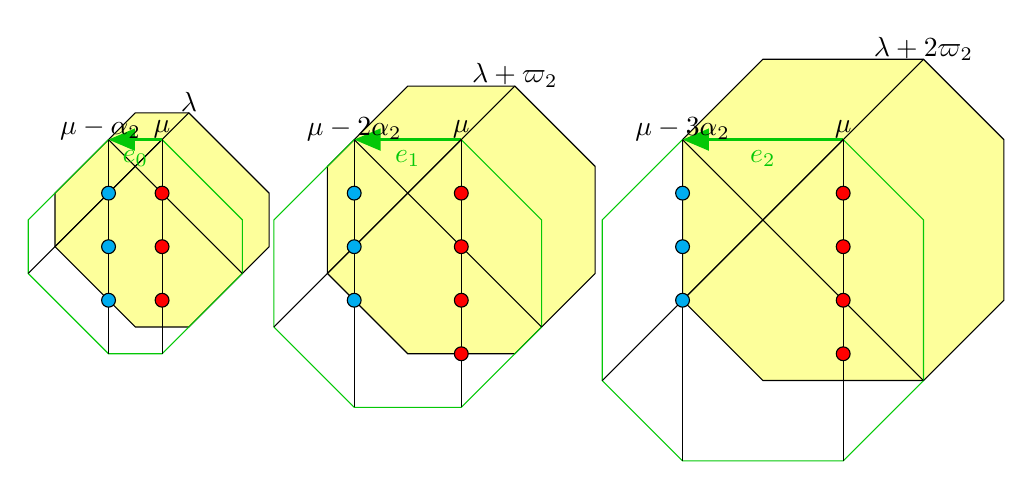
\begin{tikzpicture}[x=0.17cm,y=0.17cm]
\draw[black] (2,8) -- (-2,8) -- (-8,2) -- (-8,-2) -- (-2,-8) -- (2,-8) -- (8,-2) -- (8,2) -- cycle;
\draw[green] (-10,-4) -- (-10,0) -- (-4,6) -- (0,6) -- (6,0) -- (6,-4) -- (0,-10) -- (-4,-10) -- cycle;
\draw  (0,6)-- (-10,-4);
\draw  (0,6)-- (0,-10);
\draw  (-4,6)-- (-4,-10);
\draw  (-4,6)-- (6,-4);
\draw  (-8,-2)-- (2,8);
%\draw [fill=red] (0,6) circle (2.5pt);
%\draw [fill=cyan] (-4,6) circle (2.5pt);
\draw[green, very thick, -triangle 45] (0,6)  to node[below,color=mygreen] {$e_0$} (-4,6);
\node at (2,8.8) {$\lam$};
\node at (0,6.8) {$\mu$};
\node at (-4.6,6.8) {$\mu-\alpha_2$};

\draw [fill=cyan] (-4,-6) circle (2.5pt);
\draw [fill=cyan] (-4,2) circle (2.5pt);
\draw [fill=red] (0,2) circle (2.5pt);
\draw [fill=red] (0,-2) circle (2.5pt);
\draw [fill=cyan] (-4,-2) circle (2.5pt);
\draw [fill=red] (0,-6) circle (2.5pt);
\begin{scope}[xshift=3.8cm]
\draw[black] (4,10) -- (-4,10) -- (-10,4) -- (-10,-4) -- (-4,-10) -- (4,-10) -- (10,-4) -- (10,4) -- cycle;
\draw[green] (-14,-8) -- (-14,0) -- (-8,6) -- (0,6) -- (6,0) -- (6,-8) -- (0,-14) -- (-8,-14) -- cycle;
\draw[green, very thick, -triangle 45] (0,6) to node[below,color=mygreen] {$e_1$} (-8,6);
\draw  (0,6)-- (-14,-8);
\draw  (0,6)-- (0,-14);
\draw  (-8,6)-- (-8,-14);
\draw  (-8,6)-- (6,-8);
\draw  (-10,-4)-- (4,10);
%\draw [fill=cyan] (4,10) circle (2.5pt);
\node at (4,10.8) {$\lam+\varpi_2$};
\node at (0,6.8) {$\mu$};
\node at (-8,6.8) {$\mu-2\alpha_2$};
%\draw [fill=red] (0,6) circle (2.5pt);
%\draw [fill=cyan] (-8,6) circle (2.5pt);
\draw [fill=cyan] (-8,-6) circle (2.5pt);
\draw [fill=cyan] (-8,-2) circle (2.5pt);
\draw [fill=red] (0,-2) circle (2.5pt);
\draw [fill=red] (0,2) circle (2.5pt);
\draw [fill=cyan] (-8,2) circle (2.5pt);
\draw [fill=red] (0,-6) circle (2.5pt);
\draw [fill=red] (0,-10) circle (2.5pt);
\end{scope}
\begin{scope}[xshift=8.65cm]
\draw[black] (6,12) -- (-6,12) -- (-12,6) -- (-12,-6) -- (-6,-12) -- (6,-12) -- (12,-6) -- (12,6) -- cycle;
\draw[green] (-18,-12) -- (-18,0) -- (-12,6) -- (0,6) -- (6,0) -- (6,-12) -- (0,-18) -- (-12,-18) -- cycle;
\draw[green, very thick, -triangle 45] (0,6) to node[below,color=mygreen] {$e_2$} (-12,6);
\draw  (0,6)-- (-18,-12);
\draw  (0,6)-- (0,-18);
\draw  (-12,6)-- (-12,-18);
\draw  (-12,6)-- (6,-12);
\draw  (-12,-6)-- (6,12);
\node at (6,12.8) {$\lam+2\varpi_2$};
\node at (0,6.8) {$\mu$};
\node at (-12,6.8) {$\mu-3\alpha_2$};
%\draw [fill=cyan] (6,12) circle (2.5pt);
%\draw [fill=red] (0,6) circle (2.5pt);
%\draw [fill=cyan] (-12,6) circle (2.5pt);
\draw [fill=cyan] (-12,-6) circle (2.5pt);
\draw [fill=red] (0,-6) circle (2.5pt);
\draw [fill=red] (0,2) circle (2.5pt);
\draw [fill=cyan] (-12,2) circle (2.5pt);
\draw [fill=red] (0,-2) circle (2.5pt);
\draw [fill=red] (0,-10) circle (2.5pt);
\draw [fill=cyan] (-12,-2) circle (2.5pt);
\end{scope}
\end{tikzpicture}
\end{center}
\caption{The edge $e_0$ is swappable while $e_1$ and $e_2$ are not. To check this, since $\mu_1\geq \lam_1$, as explained in \Cref{mu1geqlam1}, it is enough to compare the number of weight in the convex hull lying below $\mu$ and $v\mu$.} 
\label{fig:staircase}
\end{figure}

Moreover, as illustrated in \Cref{staircasemax}, the staircase $(e_1,e_2)$ cannot be extended, since $\mu-4\alpha_2\not \leq \lam+3\varpi_2$. Hence, we have $\affD_\infty(\mu,\lam)=2$.

\begin{figure}
\begin{center}
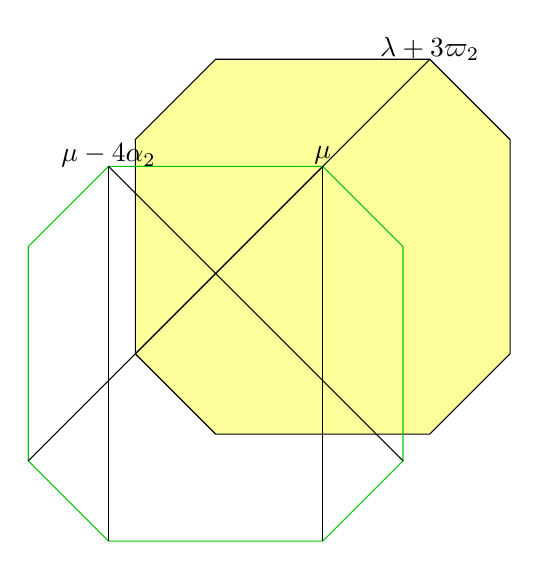
\begin{tikzpicture}[x=0.17cm,y=0.17cm]
\draw[black] (8,14) -- (-8,14) -- (-14,8) -- (-14,-8) -- (-8,-14) -- (8,-14) -- (14,-8) -- (14,8) -- cycle;
\draw[green] (-22,-16) -- (-22,0) -- (-16,6) -- (0,6) -- (6,0) -- (6,-16) -- (0,-22) -- (-16,-22) -- cycle;
\draw  (0,6)-- (-22,-16);
\draw  (0,6)-- (0,-22);
\draw  (-16,6)-- (-16,-22);
\draw  (-16,6)-- (6,-16);
\draw  (-14,-8)-- (8,14);
\node at (8,14.8) {$\lam+3\varpi_2$};
\node at (0,6.8) {$\mu$};
\node at (-16,6.8) {$\mu-4\alpha_2$};
\end{tikzpicture}
\end{center}
\caption{We have $\mu-4\alpha_2\not \leq \lam+3\varpi_2$ and the NS staircase $(e_1,e_2)$ from \Cref{fig:staircase} cannot be extended.}
\label{staircasemax}
\end{figure}

\end{example}

\begin{lemma}\label{staircaseunique}
There exists at most one non-empty NS-staircase over $(\mu,\lam)$.
\end{lemma}
\begin{proof}
Assume that the there are two non-empty NS-staircases of the form $\mu\raw \mu-(n+i)\alpha\in E^N(\lam+i\varpi_2)$ and $\mu\raw \mu-(n'+i)\beta\in E^N(\lam+i\varpi_2)$. Now, if $\mu_1> 0$, by \Cref{mu1>0nonswap2} we have $\alpha=\beta=\alpha_2$ and if $\mu_1<0$ we have $\alpha=\beta=\alpha_{12}$, so in particular $\alpha=\beta$.

We can assume $n'<n$. Since $\mu \raw \mu - n\alpha\in E^S(\lam)$, by \Cref{corcon}.1), we have that $\mu\raw \mu -n\alpha\in E^S(\lam+\varpi_2)$. With this and  \Cref{corcon}.2), we get $(\mu\raw \mu -(n'+1)\alpha)\in E^S(\lam+\varpi_2)$. Our second NS-staircase must therefore be empty. 
\end{proof}





\begin{lemma}\label{ifN=0thenD=0}
If $\calN_m(\mu,\lam)=0$ and $\mu <t_{m}\mu\leq \lam$, then also $\affD_m(\mu,\lam)=0$.
\end{lemma}
\begin{proof}
Assume that $\mu_1>0$.
If $\mu\raw t_k\mu\in E^S(\lam)$ for $k\leq m$, then also $\mu \raw t_k\mu \in E^S(\lam+\varpi_2)$ by \Cref{corcon}. If $t_k\mu\not \leq \lam$ and $(\mu\raw t_k\mu)\in E^N(\lam+\varpi_2)$, then $t_k=s_{K\delta-\alpha_2^\vee}$. But this cannot happen by \Cref{smallerissmaller}.

The case $\mu_1<0$ is symmetric.
\end{proof}

\begin{proposition}\label{Dcount}
 If $\mu_1>0$ we have
	\[ \affD_\infty(\mu,\lambda)=
	\begin{cases}
	\max(0,\min(\lam_1,\mu_1)-1) &\begin{array}{l}\text{if }-\lam_2\leq \mu_2\leq \lam_2 \\\text{ and }\mu_2\not\equiv\lam_2 \pmod{2};\end{array}\\
\max(0,\min(\mu_1,\lam_1)+\lam_2+\mu_2) &\begin{array}{l}\text{if } \mu_2<-\lam_2;\end{array}\\
0 &\begin{array}{l}\text{otherwise}.\end{array}
\end{cases}
\]
\end{proposition}
\begin{proof}
 Let $(e_i)_{1\leq i \leq a}=(\mu\raw v_{M+i}\mu)_{1 \leq i \leq a}$ be a non-empty maximal $NS$-staircase over $(\mu,\lam)$ with $M\geq -\mu_2$.

Assume first $\mu_1\geq \lam_1$. We have $e_1=(\mu\raw v_{M+1}\mu)\in E^N(\lam+\varpi_2)$, so by \Cref{mu1geqlam1} we get $\mu_2<-\lam_2$ or $M+1> \frc{\lam_2+1-\mu_2}$. We have either $v_M\mu=\mu$  or $e_0=(\mu\raw v_M\mu)\in E^S(\lam)$.
In the first case we get $-M=\mu_2$. In the second case we have $\mu_2\geq -\lam_2+1$, $M\leq \frc{\lam_2-\mu_2}$ and $M+1> \frc{\lam_2+1-\mu_2}$, so the only possibility is \[M=\frc{\lam_2-\mu_2}=\frc{\lam_2-\mu_2+1},\]
which also implies $\lam_2\not\equiv \mu_2 \pmod{2}$.

Assume further that $\mu_2<-\lam_2$.
From the discussion above we must have $M=-\mu_2$. It is easy to check that for any $k\geq 1$ we have $e_k\in E^N(\lam+k\varpi_2)$ if  $v_{M+k}\mu \leq \lam+k\varpi_2$ and that \[v_{M+k}\mu \leq \lam+k\varpi_2\iff \frf{\lam_1+\lam_2+\mu_2-k} \geq 0\]
so we get $\affD_{\infty}(\mu,\lam)=\max(0,\lam_1+\lam_2+\mu_2)$.

Assume now $\mu_2\geq -\lam_2$. If $\lam_2\not\equiv \mu_2 \pmod{2}$ then $\affD_\infty(\mu,\lam)=0$. If $\lam_2\not\equiv \mu_2 \pmod{2}$ we must have $M=\frc{\lam_2-\mu_2}$.
Since $v_M\mu\leq \lam$, from \eqref{eqtu} we get
%\[M\leq \frac{\lam_1-\mu_1}{2}-\mu_2+\min(\frf{\lam_2+\mu_1+\mu_2},\lam_2),\]
%so in particular 
\[ \frc{\lam_2-\mu_2}\leq \frf{\lam_1+\lam_2-\mu_2},\]
so this is possible only if $\lam_1 > 0$.
It easy to check that for any $k\geq 1$ if $v_{M+k}\mu \leq \lam + k\varpi_2$, then also $(\mu\raw v_{M+k}(\mu))\in E^N(\lam+k\varpi_2)$. Moreover, from \eqref{eqtu} $v_{M+k}\leq \lam+k\varpi_2$ we see that is equivalent to
%\[ \frc{\lam_2-\mu_2}\leq \frac{\lam_1-\mu_1}{2}+\frf{\lam_2+\mu_1-\mu_2+k}\]
\[\frc{\lam_2-\mu_2}\leq \frf{\lam_1+\lam_2-\mu_2-k}\]
which is true if and only if $k\leq \lam_1-1$. Hence $\affD_\infty(\mu,\lam)=\max(0,\lam_1-1)$.

The proof in the case  $0<\mu_1 < \lam_1$ is similar.
Since $e_1\in E^N(\lam+\varpi_2)$ we have $M+1>\frac{\lam_1-\mu_1}{2}+\max(-\mu_2,\frc{\lam_2-\mu_2+1})$. We have either $v_M\mu=\mu$ or $(\mu\raw v_M\mu)\in E^S(\lam)$. However, the first case is not possible because 
\[M+1=-\mu_2+1\leq \frac{\lam_1-\mu_1}{2}+\max(-\mu_2,\frc{\lam_2-\mu_2+1}).\]
In the second case, we have $M\leq \frac{\lam_1-\mu_1}{2}+\max(-\mu_2,\frc{\lam_2-\mu_2})$, which forces 
\begin{equation}\label{maxequality}
\max(-\mu_2,\frc{\lam_2-\mu_2})=(-\mu_2,\frc{\lam_2-\mu_2+1})
\end{equation}
 and $M=\frac{\lam_1-\mu_1}{2}+\max(-\mu_2,\frc{\lam_2-\mu_2}).$
The equality in \eqref{maxequality} can only occur if $\mu_2< -\lam_2$ or if $\mu_2\geq -\lam_2$ and $\lam_2\not \equiv \mu_2 \pmod{2}$.

Assume now $\mu_2<-\lam_2$. Then $M=\frac{\lam_1-\mu_1}{2}-\mu_2$. It is easy to check that for any $k\geq 1$ we have $e_k\in E^N(\lam+k\varpi_2)$ if  $v_{M+k}\mu \leq \lam+k\varpi_2$ and that \[v_{M+k}\mu \leq \lam+k\varpi_2\iff \frf{\mu_1+\lam_2+\mu_2-k} \geq 0\]
so we get $\affD_{\infty}(\mu,\lam)=\max(0,\mu_1+\lam_2+\mu_2)$.

Finally assume $\mu_2\geq -\lam_2$. If $\lam_2\not\equiv \mu_2 \pmod{2}$ then $\affD_\infty(\mu,\lam)=0$. If $\lam_2\not\equiv \mu_2 \pmod{2}$ we must have $M=\frac{\lam_1-\mu_1}{2}+\frc{\lam_2-\mu_2}$.
%\[M\leq \frac{\lam_1-\mu_1}{2}-\mu_2+\min(\frf{\lam_2+\mu_1+\mu_2},\lam_2),\]
%so in particular 
It easy to check that for any $k\geq 1$ if $v_{M+k}\mu \leq \lam + k\varpi_2$, then also $(\mu\raw v_{M+k}(\mu))\in E^N(\lam+k\varpi_2)$. Moreover, from \eqref{eqtu} $v_{M+k}\leq \lam+k\varpi_2$ we see that is equivalent to $k+1\leq \mu_1$.
 Hence $\affD_\infty(\mu,\lam)=\max(0,\mu_1-1)$.
\end{proof}

\begin{corollary}\label{Dinf<0}
If $\mu_1<0$ we have 
\begin{align*}\affD_\infty(\mu,\lambda) =\begin{cases}
	\max(0,\min(\lam_1,-\mu_1)-1) &\begin{array}{l}
 \text{if }-\lam_2\leq \mu_1+\mu_2\leq \lam_2 \\\text{and } \mu_1+\mu_2\not\equiv\lam_2 \;(\mathrm{mod }\;2);\end{array}\\
\max(0,\min(-\mu_1,\lam_1)+\lam_2+\mu_1+\mu_2) \hspace{-10pt}&\begin{array}{l}\text{if } \mu_1+\mu_2<-\lam_2;\end{array}\\
0 &\begin{array}{l}\text{otherwise}.\end{array}\end{cases}\end{align*}
\end{corollary}
\begin{proof}
    This immediately follows from \Cref{Dcount}, since by symmetry (cf. \Cref{12notswap}) we have $\affD_{\infty}(\mu,\lam)=\affD_{\infty}(s_1(\mu),\lam)$.
\end{proof}


Suppose than $T\in \calA(\lamk)\subset \calP(\lam)$.
In our applications in \Cref{sec:swapping}, we are only interested in NS staircase over $(\wt(T),\lamk)$ that live inside the preatom $\calP(\lam)$. In other words, we truncate our NS staircases $(e_i)_{1\leq i\leq a}$ so that $a\leq k$. 

The following quantity measures the longest possible truncated NS staircase over $(\mu,\lamk)$ in a preatom of highest weight $\lambda$.
\begin{definition}
\label{truncatedns}
Assume that $k\geq 0$ and $\mu \leq \lam-k\varpi_2$. Then, for any $m\in \bbN\cup \{\infty\}$ we define
\[ \calD_m(\mu,\lam,k):=\min(k,\affD_m(\mu,\lam-k\varpi_2)).\]
\end{definition}


\section{The charge and recharge statistics}\label{sec:swapping}

\subsection{A family of cocharacters}\label{sec:family}

We recall some definitions from \cite{Pat}.
Let $\affX=X\oplus \bbZ d$ be the cocharacter lattice of $T^\vee \times \bbC^*$, where $T^\vee$ is the maximal torus of $G^\vee$.
Let $\affX_\bbQ  := \affX \otimes_\bbZ \bbQ$ and $\affX_\bbR := \affX \otimes_\bbZ \bbR$.

 The \emph{KL region} is the subset of $\affX_\bbQ$ of the elements $\eta$ such that $\langle \alpha^\vee,\eta\rangle >0$ for all $\alpha^\vee \in \affPhi_+^\vee$. Concretely, an element in the KL region can be written as $\eta=\lambda+Cd$ where $\lambda\in X_{++}$ and $C>\langle \lambda,\beta^\vee\rangle$ for all $\beta^\vee \in \Phi^\vee_+$.
 The \emph{MV region} is the subset of $\affX_\bbQ$ consisting of elements of the form $\eta=\lambda+Cd$, with $\lambda\in X_{++}$ and $C=0$.

We call \emph{wall} a hyperplane in $\affX_\bbR$ of the form 
\[H_{\alpha^\vee}:=\{ \eta \in \affX_\bbR \mid \langle \eta,\alpha^\vee \rangle =0\}\subset \affX_\bbR\]
for $\alpha^\vee\in \affPhi^\vee$.
	For $\lambda\in X_+$, we denote by $\affPhi^\vee(\lambda)$ the set of all the labels present in the graph $\Gamma_\lambda$. We say that a wall $H_{\alpha^\vee}$ is a $\lambda$-wall if $\alpha^\vee\in \affPhi^\vee(\lambda)$.
We call \emph{$\lambda$-chamber} (or simply chamber, if $\lambda$ is clear from the context)  the intersection of $\affX_\bbQ$ with a connected component of 
\[\affX_\bbR \setminus \bigcup_{\alpha^\vee\in \affPhi^\vee(\lambda)}H_{\alpha^\vee}.\]
Two chambers are \emph{adjacent} if they are separated by a single $\lambda$-wall. 
The \emph{KL chamber} is the unique chamber containing the KL region and the  \emph{MV chamber} is the unique chamber containing the MV region.
We say that $\lambda\in X_\bbQ$ is \emph{regular} if it does not lie on any wall, and it is \emph{singular} otherwise.

For $\lam\in X_+$ let $\bar{\Gr^\lam}$ denote the corresponding Schubert variety in the affine Grassmannian of $G^\vee$ (cf. \cite[\S 2.1.2.]{Pat}). For any regular $\eta \in \affX$ and any $\mu \leq \lam$ the hyperbolic localization induces a functor 
\[ \HL^\eta_\mu: \calD^b_{T^\vee \times \bbC^*}(\bar{\Gr^\lam})\raw \calD^b(pt)\cong \mathrm{Vect}^\bbZ,\]
where $\calD^b_{T^\vee \times \bbC^*}(\bar{\mathcal{G}r}^\lam)$ is the derived category of $T^\vee \times \bbC^*$-equivariant constructible sheaves on the Schubert variety $\bar{\Gr^\lam}$ with $\bbQ$-coefficients, and $\calD^b(pt)$ is the derived category of sheaves on a point, which is equivalent to the category of graded $\bbQ$-vector spaces (see \cite[\S 2.4]{Pat}).
In general, for any regular $\eta\in \affX_\bbQ$ we can define $\HL^\eta_\mu$ as $\HL^{N\eta}_\mu$, where $N$ is any positive integer such that $N\eta\in \affX$. By abuse of terminology, we are then allowed to refer to all the elements in $\affX_\bbQ$ as cocharacters.

Let $\htil^\eta_{\mu,\lam}(v) := \grdim(\HL^\eta_\mu(IC_\lam))$, where $IC_\lam$ denotes the intersection cohomology sheaf on $\bar{\Gr^\lam}$. The polynomials $\htil^\eta_{\mu,\lam}(v)$ are called \emph{renormalized $\eta$-Kazhdan--Lusztig polynomials}. We say that a function $r:\calB(\lam)\raw \bbZ$ is a $\eta$-\emph{recharge} for $\eta$ if we have
\[\htil^\eta_{\mu,\lam}(q^{\frac12})=\sum_{T\in \calB(\lam)_\mu} q^{r(T)}\in \bbZ[q^{\frac12},q^{-\frac12}].\]
If $\eta_{KL}$ is in the KL chamber and $\mu \in X_+$, then
\[K_{\mu,\lam}(q)=\htil^{\eta_{KL}}_{\mu,\lam}(q^{\frac12})q^{\frac12 \ell(\mu)}\] is a Koskta--Foulkes polynomial by \cite[Proposition 2.14]{Pat}. So if $r_{KL}$ is a recharge for $\eta_{KL}$  in the KL region, we obtain a charge statistic $c:\calB(\lam)\raw \bbZ$ by setting $c(T):=r_{KL}(T)+\frac 12 \ell(\wt(T))$. 
Notice that if $\wt(T)\in X_+$ this is equal to $c(T)=r_{KL}(T)+\langle \wt(T),\rho^\vee\rangle$.


We specialize \cite[Definition 3.29]{Pat} to our setting. 
%\Jaz{There's no Section 6 in Pat new arxiv version. Are you referring to the published version?}\Leo{Corrected}

\begin{definition}
Let $\lambda\in X_+$. We call \emph{$\lambda$-parabolic region} the subset of $\affX_\bbQ$ consisting of regular cocharacters $\eta$ such that	\begin{itemize}
		\item $\langle \eta,\beta^\vee\rangle>0$ for every $\beta^\vee$ of the form 
		$M\delta -\alpha_1^\vee$ with $M>0$, or of the form $M\delta+\alpha^\vee$, with $\alpha\in \Phi_+$ and $M\geq 0$.
		\item $\langle \eta,\beta^\vee\rangle<0$ for every $\beta^\vee\in \affPhi^\vee_+(\lambda)$ of the form $M\delta-\alpha_i^\vee$ such that $M> 0$ and $i\in \{2,12,21\}$.
	\end{itemize} 
\end{definition} 


The walls that separate the  parabolic region from the KL region are precisely
\[ H_{M\delta-\alpha_i^\vee} \qquad \text{with }M>0\text{ and }i\in \{2,12,21\}.\]
Every cocharacter $\eta_P$ of the form
\[ \eta_P= A_1\varpi_1 + A_2\varpi_2 + Cd\]
with $0\ll A_1\ll C\ll A_2$ lies in the parabolic region.\footnote{More precisely, sufficient conditions are $0<A_1<C<\frac{A_2}{\gamma}$ where $\gamma=\max\{ M \mid M\delta-\beta^\vee \in \Phi^\vee(\lam)\}$.}



We consider the following family of cocharacters:
\begin{equation}\label{family}
	\eta:\bbQ_{\geq 0}\ra \affX_\bbQ,\qquad \eta(t)=\eta_P+t d.
\end{equation} 
Observe that $\eta(t)$ is in the KL chamber for $t\gg 0$. We can choose $t_0$ such that $\eta(t_0)$ is in the KL chamber and for any $i$ we choose $t_{i+1}<t_{i}$ so that $\eta(t_i)$ and $\eta(t_{i+1})$ lie in adjacent $\lambda$-chambers until we arrive at $t_M$ in the parabolic region. We can furthermore choose  $t_M=0$ and set $t_{M+1}=\ldots =t_{\infty}=0$ and $\eta_i:=\eta(t_i)$ for any $i\in \bbN \cup \{\infty\}$.

\subsection{Recharge statistics from the parabolic to the KL region}



Our goal is to attach a recharge statistic to each of the cocharacters $\eta_i$. 

Let $T\in \calB(\lambda)$. Recall that by \Cref{preatomicnumber,defatomicnumber} we have 
\[T\in \calA(\lam-\at(T)\varpi_2-2\pat(T) \varpi_1)\subset \calP(\lam-2\varpi_1(T))\subset \calB(\lam).\]


\begin{definition}\label{N=0}
Assume that $T\in  \calP(\lam)\subset \calB(\lam')$ with $\mu:=\wt(T)$. Let $a:=\at(T)$ and $p:=\pat(T)$ so that $\lam'=\lam+2p\varpi_1$. We define
\[ \sigma_m(T):= \ell_m(\mu,\lama)-\calN_m(\mu,\lama)+\calD_m(\mu,\lambda,a)+a+2p.\]
Let $r_m(T):=-\sigma_m(T)+\langle \lam',\rho^\vee\rangle=-\sigma_m(T)+\langle \lam,\rho^\vee\rangle+3p$.

\end{definition}

Our main result is the following.

\begin{theorem}
\label{maintheorem}
The function $r_m:\calB(\lambda)\raw \bbZ$ is a recharge statistic for $\eta_m$ for any $m\in \bbN\cup \{\infty\}$.
\end{theorem}

The proof that $r_i$ is a recharge for $\eta_i$ is divided in two parts. We first show directly in \Cref{sec:parabolic} that $r_\infty$ is a recharge statistic for $\eta_\infty=\eta(0)$, i.e. a recharge in the parabolic region, and then we construct for any $i$ swapping functions between $\eta_i$ and $\eta_{i+1}$. 
After putting everything together, this proves that $r_{KL}:=r_0$ is a recharge in the KL region, and we can easily obtain from that the following formula for a charge statistic in type $C_2$.

\begin{corollary}
\label{maincharge}
The function
$c:\calB(\lam)_+\raw \bbZ$ defined as
\[c(T)=\langle \lambda -\wt(T),\rho^\vee\rangle -\at(T)-\pat(T)\]
is a charge statistic.
\end{corollary}
\begin{proof}
By definition, we have $\calN_0=\calD_0=0$ and $\ell_0=\ell$. Hence
\[ c(T)=r_0(T)+\frac12\ell(\wt(T))=\langle \lambda,\rho^\vee\rangle -\frac12\ell(\wt(T))-\at(T)-2\pat(T)\]
is a charge statistic. We conclude since, for $T=\calB(\lam)_+$, we have $\ell(\wt(T))=2\langle \wt(T),\rho^\vee\rangle$.
\end{proof}




\subsection{Recharge in the parabolic region}\label{sec:parabolic}

Let $\eta_{MV}$ be a cocharacter in the MV region and $\eta_P$ be in the parabolic region. The only walls separating $\eta_{MV}$ from $\eta_P$ are of the form $H_{M\delta-\alpha_1^\vee}$, with $M>0$. We now from  \cite[Eq. (17)]{Pat} that
\[r_{MV}(T) = -\langle \rho^\vee, \wt(T)\rangle.\] 
is a recharge in the MV region. To construct a recharge in the parabolic region, after Levi branching, we can assume we are in rank $1$ and thus compute the recharge as illustrated in \cite[\S 3.4]{Pat}. In particular, it follows from \cite[Lemma 3.26]{Pat} that 
\[ r_P(T)=-\langle \rho^\vee,\wt(T)\rangle+\phi_1(T)-\ell^1(\wt(T))\]
is a recharge in the parabolic region. It remains to show the equality between $r_P$ and $r_{\infty}$.


% \begin{definition}
%     Assume $T\in \calA(\lam)$. For $i \in \{2,12,21\}$ let $\affphi_i(T):=\affphi_i(\wt(T),\lam)$.
% \end{definition}

%Let $T\in \calA(\lam-k\varpi_2)\subset \calP(\lam)\subset \calB(\lam')$. 
Let $T\in \calP(\lam)\subset \calB(\lam+2p\varpi)$ with $p=\pat(T)$ and let $a=\at(T)$ and $\mu=\wt(T)$.
At $m=\infty$, we have 
\begin{align}\label{sigmainf}
 \sigma_\infty(T) = \ell^1(\mu)+  \sum_{i\in \{2,12,21\}}\affphi_i(\mu,\lama) \nonumber \\
 -\calN_\infty(\mu,\lama)+\calD_\infty(\mu,\lam,a)+a+2p.
 %&=\ell^1(\mu)+\sum_{i\in \{2,12,21\}}\affphi_i(T)-\calN_\infty(\mu,\lama)+\calD_\infty(\mu,\lam,a)+a+2p
\end{align}

Our next goal is to simplify the expression \eqref{sigmainf}.

\begin{lemma}\label{phi21k}
We have $\affphi_{21}(\mu,\lama)+a=\affphi_{21}(\mu,\lambda)$.
\end{lemma}
\begin{proof}
    This follows directly from \Cref{affphicompute}.
\end{proof}


\begin{proposition}\label{phi12hard}
Let $\mu = \wt(T)$ and assume that $\mu_1\leq  0$. We have $\phi_2(T)=\affphi_2(\mu,\lama)$ and
\[\phi_{12}(T)=\affphi_{12}(\mu,\lama)-\calN_\infty(\mu,\lama)+\calD_\infty(\mu,\lambda,a).\]
\end{proposition}
The proof of \Cref{phi12hard} is rather long and technical and we postpone it to \Cref{sec:phi2}.

\begin{lemma}\label{sigmainfnicelemma}
Let $\mu=\wt(T)$. We have 
\begin{equation}\label{sigmainfnice}\sigma_\infty(T)=\ell^1(\mu)+\phi_2(T)+\phi_{12}(T)+\affphi_{21}(\mu,\lambda)+2p.
\end{equation}
\end{lemma}
\begin{proof}
If $\mu_1\leq 0$, this follows immediately from \Cref{phi21k} and \Cref{phi12hard}.

If $\mu_1>0$, then let $T'=s_1(T)$. Recall that atoms are stable under $s_1$ by \Cref{lemmaonPsi}. So the element $T'$ can also be characterized as the element in the same atom of $T$ with weight $s_1(\mu)$. %\Leo{Argh, there is maybe a  small problem in the definition of $\at$. We want them to be stable under $s_1$ so the definition we gave only work for $\mu_1\geq 0$. (Or $\mu_1\leq 0$?)}
Notice that $\affphi_{21}$, $\calN_\infty$ and $\calD_\infty$ are preserved by $s_1$, while  $\affphi_{2}(\mu,\lama)=\affphi_{12}(s_1(\mu),\lama)$ and $\ell^1(\mu)=\ell^1(s_1(\mu))- 1$. It follows that $\sigma_\infty(T)=\sigma_\infty(T')-1$. On the other hand, we also have $\phi_2(T)=\phi_{12}(T')$ and $\phi_{12}(T')=\phi_2(T)$, so we obtain the desired identity \eqref{sigmainfnice} for $T$ as well.
\end{proof}

\begin{proposition}\label{rP}
We have $r_P(T)=r_\infty(T)$ for any $T \in \calB(\lambda')$.
\end{proposition}
\begin{proof}
Let $\mu=\wt(T)$ and assume $T\in \calP(\lam)\subset \calB(\lam+2p\varpi_1)$. By \Cref{sigmainfnicelemma} we have
\[r_\infty(T)=-\ell^1(\mu)-\phi_2(T)-\phi_{12}(T)-\affphi_{21}(\mu,\lam)+\langle \lam,\rho^\vee\rangle+p.\]
So our claim is equivalent to
\[ \langle \lambda+\mu,\rho^\vee \rangle -\affphi_{21}(\mu,\lam)=\phi_1(T)+\phi_2(T)+\phi_{12}(T)-p=Z(T)-p.\]
By  \Cref{atomicnumber} and \Cref{affphicompute} we have
\begin{align*}\langle \mu+\lam,\rho\rangle -\affphi_{21}(\mu,\lam)%&=\frac32(\lam_1+\mu_1)+\lam_2+\mu_2-\min(\lam_1,\frac{\lam_1+\mu_1}{2},\lam_1+\mu_1)\\
		&= \lam_2+\mu_2+\frac32\lam_1+\frac32\mu_1-\min(\lam_1,\frac{\lam_1+\mu_1}{2},\lam_1+\mu_1)\\
		&= \lam_2+\mu_2+\lam_1+\mu_1-\min(\frac{\lam_1-\mu_1}{2},0,\frac{\lam_1+\mu_1}{2})\\
  & =Z(T) - p.\qedhere
\end{align*}
\end{proof}


\subsection{Computing \texorpdfstring{$\phi_2$}{psi}}
\label{sec:phi2}
It remains to prove the identity \Cref{phi12hard}.

We begin by considering the case $\at(T)=0$. The general case will follow by induction on the atomic number.





\begin{proposition}\label{atomicphi2}
    For any $T \in \calP(\lam)$ with $\wt(T)_1\leq 0$ we have $\phi_2(T)=\affphi_2(\wt(T),\lam-\at(T)\varpi_2)$.
\end{proposition}

\begin{proof}
Let $\mu \leq \lam$. Consider the multiset
\[ M_2(\mu,\lam):=\{ \phi_2(X) \mid X \in \calP(\lambda)\text{ with }\wt(X)=\mu\}\]
Since $\calP(\lambda)$ is a union of $f_2$-strings, we have an equality of multisets
\begin{equation}\label{M2alt}M_2(\mu,\lam)=\{\affphi(\mu,\lamk) \mid 0\leq k\leq \lam_2 \text{ with }\mu \leq \lamk\}.
\end{equation}
In fact, the $f_2$-strings contained in $\calP(\lambda)$ which pass through an element of weight $\mu$ are in bijection with the atoms in $\calP(\lambda)$ containing an element of weight $\mu$.

The claim now follows by induction on $\lam_2$. If $\lam_2=0$, then $\calP(\lambda)=\calA(\lambda)$ and $M_2(\mu,\lambda)=\{\phi_2(T)\} =\{\affphi_{2}(\mu,\lam)\}$.

If $\lam_2>0$, consider the embedding $\Psi:\calP(\lam-\varpi_2)\hookrightarrow \calP(\lam)$ from \Cref{defPsi}. The map $\Psi$ is weight preserving and we have  $\phi_2(\Psi(X))=\phi_2(X)$ and $\at(\Psi(X))=\at(X)+1$ for any $X\in \calP(\lam-\varpi_2)$ with $\wt(X)_1\leq 0$. 
If $T= \psi(X)$ for some $X\in \calP(\lam-\varpi_2)$, then $\phi_2(T)=\phi_2(X)=\affphi_2(\mu,\lam-\varpi_2-\at(X)\varpi_2)$ and the claim follows. Otherwise, we have $T\in \calA(\lam)=\calP(\lam)\setminus \Psi(\calP(\lam-\varpi_2))$
and by \eqref{M2alt} we see that
\[ \{\phi_2(T)\}=M_2(\mu,\lam)\setminus M_2(\mu,\lam-\varpi_2)=\{ \affphi_2(\mu,\lam)\}.\qedhere\]
\end{proof}


\begin{lemma}\label{phi1at0}
Let $T\in \calP(\lam)\subset \calB(\lam)$ and let $\mu=\wt(T)$. Assume $\mu_1< 0$ and $\at(T)=0$. Then we have $
    \phi_1(T) = \max(0,\mu_1+\mu_2-\lam_2,-\mu_2-\lam_2).$
\end{lemma}
% \begin{align}
% \phi_1(T) &= \max(0,\mu_1+\mu_2-\lam_2,-\mu_2-\lam_2),\label{claim0}\\ \phi_{12}(T) &= \affphi_{12}(\mu,\lam)-\calN_{\infty}(\mu,\lam).\label{claim12}
% \end{align}

\begin{proof}

%It is enough to prove the claims for $\pat(T)=0$. Otherwise $T=\Phi(T')$ and by induction we have $\phi_1(T)=\phi_1(T')+1$ and $\phi_{12}(T)=\phi_{12}(T')$.

Let $\stn(T)=(a,b,c,d)$.
By \Cref{atom0} we have 
\[\at(T)=0\iff (c=d=0) \text{ or }(b=\lam_1+2c-2d\text{ and }d\leq 1\text{ or }c= \lam_2+d)\]

As computed in \eqref{phi1stn}, we have
\[\phi_1(T)=\lam_1+2a-2b+2c-2d+\max(d,2c-b,b-2a).\]

%so the claim is equivalent to
%\[\lam_1+2a+4c-b-d-\min(2a+2c+d,b+2c,2b+d) = \max(0,\lam_1-b-d,-2\lam_2-b-d+2a+2c).\]
We now divide into several cases. 
Assume first $c=d=0$. Then the statement is equivalent
\begin{equation}\label{eqcd0}\lam_1+2a-b-\min(2a,b) = \max(0,\lam_1-b,-2\lam_2-b+2a).\end{equation}
Since $\mu_1=\lam_1-2b+2a <0$ and $b\leq \lam_1$, we have $2a\leq b$, so the LHS in \eqref{eqcd0} is $\lam_1-b$.
Moreover, $\lam_1-b\geq 0$ and $\lam_1-b\geq 2a-b-2\lam_2$ otherwise we get.
$\lam_1+2\lam_2< 2a<b.$ So the RHS in \eqref{eqcd0} is also equal to $\lam_1-b$.

We can now assume $b=\lam_1+2c-2d$, so we have
$\phi_1(T)=\max(-\lam_1+2a-2c+3d,0)$,
while the RHS  can be rewritten as 
$\max(0,d-2c,-2\lam_2+d+2a-\lam_1)$.
Moreover, we have $d-2c\leq 0$ and $\mu_1 = -\lam_1+2a-2c+2d\leq 0$.
%and $2a-2\lam_1-2c+4d\leq 2a-2\lam_1-2c+2d+2b=-\mu_1-\lam_1\leq 0$.

So it is enough to show that 
\begin{equation}\label{eq2}\max(0,\mu_1+d)=\max(0,\mu_1-2(c-\lam_2-d)+d)\end{equation}
The equality is clear if $c=\lam_2+d$ and it also follows if $d\leq 1$ since that both term vanish for $\mu_1<0$.%\Leo{Is this really false if $\mu_1=0$ land $d=1$? Weirdly enough yes, e.g. for (5,10,2,1) and $\lam=(8,4)$. It should not be a problem.}
\end{proof}
%
% In the case $c= \lam_2+d$ the equation \eqref{eq2} becomes clearly an identity. 
% %\[\max(0,2a-\lam_1-2\lam_2+d)=\max(0,-2\lam_2+d+2a-\lam_1)\]
% We finally assume $d\leq 1$. In this case  implies $2a+2d\leq \lam_1+2c\leq  \lam_1+2\lam_2+2d$, hence $2a+3d\leq \lam_1+2c$. On the other hand
% $d+2a< \lam_1 +2\lam_2+1$, so $\lam_1+2\lam_2\geq d+ 2a$.\Leo{Need to check again these computations!}

\begin{proposition}
\label{phi12at0}
Let $T\in \calP(\lam)$ and let $\mu=\wt(T)$. Assume $\mu_1\leq  0$ and $\at(T)=0$. Then we have $\phi_{12}(T)=\affphi_{12}(\mu,\lam)-\calN_{\infty}(\mu,\lam).$
\end{proposition}
\begin{proof}
If $\mu_1=0$, then $\phi_{12}(T)=\phi_2(T)$, $\affphi_{12}(T)=\affphi_{2}(T)$ and $\calN_\infty(\mu,\lam)=0$, so the claim follows from \Cref{atomicphi2}. We assume in the rest of the proof $\mu_1<0$. We can also assume that $T$ lies in the biggest preatom, i.e. that $\calP(\lam)\subset \calB(\lam)$. In fact, since $\Phi$ commutes with $s_1$ and $f_2$, the claim for the other preatoms easily follows by induction.

Recall now by \Cref{atomicphi2} that $\phi_2(T)=\affphi_2(\mu,\lam)$. We divide into three cases.

We assume first $\mu_1+\mu_2\leq \lam_2$ and $\mu_2\geq -\lam_2$. Notice that this precisely means that $\phi_1(T)=0$. By \Cref{Ninf}, we have in this case
\[ \affphi_{12}(T)-\calN_\infty(\mu,\lam)=\max(0,\frf{\lam_2+\mu_1+\mu_2})-\min(0,\frac{-\lam_1-\mu_1}{2}).\]
Let $\chi:=\lam_2+\mu_1+\mu_2$. Then by \Cref{atomicnumber,atomicphi2,phi1at0} we have
\begin{align*} \phi_{12}(T) &=Z(T)-\phi_1(T)-\phi_2(T)\\
&=\frac{\lam_1+\mu_1}{2}+\chi +\max(0,\frac{-\mu_1-\lam_1}{2})-\min(\chi,\frf{\chi},\lam_2).
\end{align*}

Notice that $\min(0,\frac{-\lam_1-\mu_1}{2})+\max(0,\frac{-\lam_1-\mu_1}{2})=\frac{-\lam_1-\mu_1}{2}$ and that $\lam_2\geq \frf{\chi}$. So our claim results equivalent to the easy-to-check identity
\[\chi -\min(\chi,\frf{\chi})=\max(0,\frc{\chi}).\]

We now assume that $\mu_1+\mu_2> \lam_2$ or that $\mu_2<-\lam_2$. In both cases we have from \Cref{octineq} that $\mu_1>-\lam_1$, so $Z(T)=\lam_1+\lam_2+\mu_1+\mu_2$. Moreover, we have from \Cref{Ncount} that $\calN_{\infty}(\mu,\lam)=0$, so the claim is equivalent to $Z(T)-\phi_1(T)-\phi_2(T)=\affphi_{12}(T)$.

If $\mu_1+\mu_2>\lam_2$, then 
$\affphi_2(T)=\frac{\lam_1-\mu_1}{2}+\lam_2$ and $\affphi_{12}(T)=\frac{\lam_1+\mu_1}{2}+\lam_2$, so the desired equality reduces to the identity
\[ \lam_1+\lam_2+\mu_1+\mu_2-\mu_1-\mu_2+\lam_2-\frac{\lam_1}{2}+\frac{\mu_1}{2}-\lam_2=\frac{\lam_1}{2}+\frac{\mu_1}{2}+\lam_2.\]
Finally, if $\mu_2<-\lam_2$, the desired equality reduces to the identity
 \[ \lam_1+\lam_2+\mu_1+\mu_2+\mu_2+\lam_2-\frac{\lam_1}{2}+\frac{\mu_1}{2}-\mu_1-\mu_2-\lam_2=\frac{\lam_1}{2}+\frac{\mu_1}{2}+\lam_2+\mu_2.\qedhere\]
\end{proof}



\begin{proposition}\label{phi2claim}
Let $T\in \calP(\lam)$ and let $\mu=\wt(T)$. Let $A:=\at(T)$.
	If $\mu_1\leq 0$, we have
\[\phi_{12}(T)=\affphi_{12}(\mu,\lam- A\varpi_2)-\calN_\infty(\mu,\lambda-A\varpi_2)+\calD_\infty(\mu,\lambda,A).\]
\end{proposition}

\begin{proof}
As in \Cref{phi12at0} we can assume that $\calP(\lam)\subset \calB(\lam)$.
We show the claim it by induction on $A$.
	If $A=0$, the claim immediately follows from \Cref{phi1at0} since $\calD_\infty(\mu,\lam,0)=0$. 

 If $A>0$, then $T=\Psi(U)$ for some $U\in \calP(\lambda-\omega_2)\subset \calB(\lam-\omega_2)$ with $\at(U)=A-1$.
By induction, we have 
\[ \phi_{12}(U)=\affphi_{12}(\mu,\lamA)-\calN_\infty(\mu,\lamA)+\calD_{\infty}(\mu,\lam-\varpi_2,A-1).\]
 So it suffices to show that, for any $U$ in $\calP(\lam-\varpi_2)\subset \calB(\lam-\varpi_2)$ with $\wt(U)=\mu$, we have
\begin{align}\label{Psiphi12} \phi_{12}(\Psi(U))-\phi_{12}(U) &=\calD_\infty(\mu,\lambda,A)-\calD_{\infty}(\mu,\lam-\varpi_2,A-1)\\
& =\min(A,\affD_\infty(\mu,\lamA))-\min(A-1,\affD_\infty(\mu,\lamA)).\nonumber\end{align}

Let $\stn(U)=(a,b,c,d)$. We know from \Cref{cor:phi12psi} that 
\[ \phi_{12}(\Psi(U))-\phi_{12}(U)=\begin{cases}
1& \text{if }d=0\text{ and }2a>b>2c\text{ or }d\neq 0,\lam_1\text{ and }b\geq 2a+d\\
0&\text{otherwise}.
\end{cases}\]
However, notice that we cannot have $d=0$ and $2a>b>2c$ since otherwise
$\mu_1=\lam_1+2a-2b+2c> \lam_1+2c-b\geq 0$.
It follows that \eqref{Psiphi12} is equivalent to showing that
\[ \affD_\infty(\mu,\lamA)\geq A \iff d\neq 0,\lam_1 \text{ and }b\geq 2a + d.\]
We show this in the following lemma.
\end{proof}

\begin{lemma}
Let $X\in \calP(\lam)\subset \calB(\lam)$ with $\mu=\wt(X)$ such that $\mu_1< 0$. Let $A:=\at(X)$ and $\stn(X)=(a,b,c,d)$. We have 
\[\affD_\infty(\mu,\lamA)> A \iff d\neq 0,\lam_1 \text{ and }b\geq 2a + d.
\]
\end{lemma}
\begin{proof}

Recall from \Cref{Dinf<0} that we have 
\[\affD_\infty(\mu,
\lamA)=\begin{cases}
	\max(0,\min(\lam_1,-\mu_1)-1) &\begin{array}{l}\text{if }\mu_1+\mu_2+\lam_2\geq A,\\
 \mu_1+\mu_2+A\leq \lam_2 \text{ and }\\
 \mu_1+\mu_2\not\equiv\lam_2-A \pmod{2};\end{array}\\
\begin{aligned}\max(0,\min(-\mu_1,\lam_1)+\lam_2\\-A+\mu_1+\mu_2) \end{aligned}&\begin{array}{c}\text{if } \mu_1+\mu_2+\lam_2<A;\end{array}\\
0 &\begin{array}{c}\text{otherwise.}\end{array}\end{cases}\]
Moreover,  from \Cref{atomformula} we have
\[A= \at(X)=\begin{cases} \min(c,\lam_1+2c-b)& \text{if }d=0\\
\lam_1+2c-2d-b+\min(\lam_2+d-c,d-1) &\text{if }d>0.\end{cases}\]

We divide the proof into three cases.

\noindent \textbf{First case: $d=0$.\;}
 We claim that in this case we  actually have $\affD_\infty(\mu,\lamA)=0$.
Notice that $\mu_1+\mu_2+\lam_2=\lam_1+2\lam_2-b\geq \lam_1+2c-b\geq A$. So we can also assume that $A\leq \lam_2-\mu_1-\mu_2=b-\lam_1$. Notice that this is equivalent to $c+\lam_1\geq b$ and $A=\lam_1+2c-b$. However, if $A=\lam_1+2c-b$ then $\mu_1+\mu_2+\lam_2+A\equiv 0 \pmod{2}$, and therefore $\affD_\infty(\mu,\lam-A\varpi_2)=0$.

\noindent \textbf{Second case: $d=\lam_1$.\;} In this case we have $A=\min(\lam_2+c-b,2c-b-1)$ and $\mu_1+\mu_2+\lam_2=2\lam_2-b$. It follows that $\mu_1+\mu_2+\lam_2\geq A$ if and only if $\lam_2\geq c$. Recall also that $b\leq 2c-\lam_1$.

Assume first $\lam_2\geq c$, so that $A=2c-b-1$ and $\mu_1+\mu_2+\lam_2\geq A$. The claim now follows since $\affD_\infty(\mu,\lam-A\varpi_2)\leq \lam_1-1\leq 2c-b-1$.

Assume now $\lam_2<c$ so that $A=\lam_2+c-b$ and $\mu_1+\mu_2+\lam_2\leq A$. The claim follows because, if $\affD_\infty(\mu,
\lamA)\geq 0$, then 
$\affD_\infty(\mu,
\lamA)\leq \lam_1+\lam_2+\mu_1+\mu_2-A=\lam_1+\lam_2-c\leq \lam_2+c-b=A$.

\noindent \textbf{Third case: $d\neq 0,\lam_1$.\;}
In this case we have $b=\lam_1-2d+2c$. Notice that $b\geq 2a+d$ is equivalent to $\lam_1-2a+2c> 3d$. We also have $A=\min(\lam_2+d-c,d-1)$ and $\mu_1+\mu_2+\lam_2=2\lam_2-2c+d$, so $\mu_1+\mu_2+\lam_2\geq A$ if and only if $\lam_2\geq c$.

Assume first $\lam_2\geq c$, so that $A=d-1$ and $\mu_1+\mu_2+\lam_2\geq A$. Notice that $\lam_1-1>A$ and also \[-\mu_1-1>A\iff \lam_1+2c-2a-2d-1>d-1\iff \lam_1+2c-2a>3d\]
Hence, $\affD_\infty(\mu,\lamA)>A$ if and only if $\lam_1+2c-2a>3d$.

Finally assume $\lam_2<c$ so that $A=\lam_2+d-c$ and $\mu_1+\mu_2+\lam_2<A$. In this case we have $\affD_\infty(\mu,\lamA)=\max(0,\min(0,\mu_1+\lam_1)+\lam_2+\mu_2-A)$.
We have $\mu_1+\lam_1+\lam_2+\mu_2-A=\lam_1+\lam_2-c>\lam_2+d-c=A$ and
\[\lam_2+\mu_2-A>A\iff \lam_1+2c-2a> 3d.\]
It follows that $\affD_\infty(\mu,\lamA)>A$ if and only if $\lam_1+2c-2a>3d$.
\end{proof}



\section{Swapping functions}

Recall the family of cocharacters $\{\eta_m\}_{m\in \bbN}$ introduced in \Cref{sec:family}.
The unique wall separating $\eta_m$ and $\eta_{m+1}$ is 
$H_{\alpha_{m+1}^\vee}$, where $\alpha_{m+1}^\vee \in \affPhi^\vee_+$ is the $(m+1)$-th root occurring in the sequence \eqref{reflectionorder}.  
As in \eqref{tm}, let $t:=t_{m+1}$  denote the corresponding reflection.
 For any $\mu\in X$ such that $\mu<t\mu\leq \lambda$ we define
\[ \psi_{t\mu}:\calB(\lambda)_{t\mu}\ra 
\calB(\lambda)_{\mu}\]
as follows. 
Let $T\in \calB(\lam)_{t\mu}$ and assume that $T\in \calA(\lam-a\varpi_2)\subset \calP(\lam)$ and let $e:=(\mu \raw t\mu)\in E(\lambda-a\varpi_2)$. Then $\psi_{t\mu}(T)=T'$, where $T'$ is the only element of weight $\mu$ in $\calA(\lam-(a+\Omega(e))\varpi_2)\subset \calP(\lam)$.

\begin{proposition}\label{swappingfunctionprop}
The collection of maps $\psi=\{\psi_\nu\}$ is a swapping function between $\eta_{m+1}$ and $\eta_m$. In particular, if $r_{m+1}$ is a recharge for $\eta_{m+1}$ then $r_m$ is a recharge for $\eta_m$. 
\end{proposition}

To prove \Cref{swappingfunctionprop} we need to check that for any $m$ and $T$ we have $r_{m+1}(T)=r_{m+1}(\psi_{t\mu}(T))+1$, or equivalently that $\sigma_{m+1}(T)=\sigma_{m+1}(\psi_{t\mu}(T))-1$. %This is in turn equivalent to $\sigma_{m}(\psi_{t\mu}(T))=\sigma_{m}(T)-1$\Leo{Is this clear?}














% Now, we need to divide into two cases.
% First we consider the case of a swappable edge, for which the swapping function only involves element within the same atom.

% \begin{proposition}
% Assume $T\in \calA(\lam-k\varpi_2)\subset \calP(\lam)$ with $t_{m+1}\mu =\wt(T)$ and that $(\mu\raw t_{m+1}\mu)\in E^S(\lam-k\varpi_2)$. Let $T$ be the element in the same atom of $T$ with weight $\mu$. Then we have
% \[\sigma_m(T)=\sigma_m(T')+1\]
% \end{proposition}
% \begin{proof}
% Since $\mu\raw t_m\mu$ is swappable we have $\ell_m(\mu,\lambda-k\varpi_2)=\ell_m(t_{m+1}\mu,\lamk)-1$. By \Cref{corcon} we have that  $\calN_m(\mu,\lambda-k\varpi_2)=0$ and by \Cref{Nintmuis0} we get $\calN_m(t_m\mu,\lamk)=0$. Finally, by \Cref{ifN=0thenD=0}, we also get $\calD_m(\mu,\lam,k)=\calD_m(t_{m+1}\mu,\lam,k)=0$ and the claim follows.
% \end{proof}

% \begin{proposition}
% Assume $T\in \calA(\lam-k\varpi_2)\subset \calP(\lam)$ with $t_{m+1}\mu =\wt(T)$ and that $(\mu\raw t_{m+1}\mu)\in E^S(\lam-k\varpi_2)$. Let $T$ be the element in the same atom of $T$ with weight $\mu$. Then we have
% \[\sigma_{m+1}(T)=\sigma_{m+1}(T')-1\]
% \end{proposition}
% \begin{proof}
% Since $\mu\raw t_m\mu$ is swappable we have $\ell_{m+1}(\mu,\lambda-k\varpi_2)=\ell_{m+1}(t_{m+1}\mu,\lamk)+1$. By \Cref{corcon} we have that  $\calN_{m+1}(\mu,\lambda-k\varpi_2)=0$ and by \Cref{Nintmuis0} we get $\calN_{m+1}(t_m\mu,\lamk)=0$. Finally, by \Cref{ifN=0thenD=0}, we also get $\calD_{m+1}(\mu,\lam,k)=\calD_{m+1}(t_{m+1}\mu,\lam,k)=0$ and the claim follows.
% \end{proof}

% We now consider the general case. \Leo{Is the first case necessary?}

% \begin{proposition}
% Assume $T\in \calA(\lam-k\varpi_2)\subset \calP(\lam)$ with $t_{m+1}\mu =\wt(T)$ and that $(\mu\raw t_{m+1}\mu)\in E^N(\lamk)$. Let $\Omega:=\Omega(\mu\raw t_{m+1}\mu)$ be its elevation.
% Let $T'$ be the element of weight $\mu$ in the atom of $\calA(\lam-(k+\Omega)\varpi_2)$.
% Then, we have 
% \begin{equation}\label{sigmans}\sigma_m(T)=\sigma_m(T')+1.\end{equation}
% \end{proposition}
% \begin{proof}
% %First of all, notice that such element $T'$ exists. In fact, we have $\mu\leq \lambda_i-k\varpi_2$. \Leo{better to prove it explicitly...} 

% By definition we have $\calD_m(\mu,\lam,k+\Omega)=\Omega-1$.
% Combining with \Cref{N=0}, our claim  \eqref{sigmans} becomes equivalent to
% \[\ell_m(t_{m+1}\mu,\lamk)=\ell_m(\mu,\lam-(k+\Omega)\varpi_2)+2\Omega-\calN_m(\mu,\lam-(k+\Omega)\varpi_2)\]

% Assume now $\mu_1>0$. By \Cref{corcon}, if $t_{m+1}\mu\leq \lam-(k+\Omega)\varpi_2$ we have $\mu \raw t_{m+1}\mu\in E^N(\lam-(k+\Omega)\varpi_2)$, so \Leo{k should be $a$}
% \[\calN_{m+1}(\mu,\lam-(k+\Omega)\varpi_2)-\calN_m(\mu,\lam-(k+\Omega)\varpi_2)=1-I_{\not\leq (\lambda-(k+\Omega)\varpi_2)}(t_{m+1}\mu)\]

% Using \Cref{Ncountgen}, this is equivalent to
% \[\ell_m(t_{m+1}\mu,\lamk)-\affell_m(t_{m+1}\mu,\lam-(k+\Omega)\varpi_2)=2\Omega-I_{\not\leq (\lambda-(k+\Omega)\varpi_2)}(t_{m+1}\mu)\]
% We can now conclude because 
% \[\affphi_{21}(t_{m+1}\mu,\lamk)-\affphi_{21}(t_{m+1}\mu,\lam-(k+\Omega)\varpi_2)=\Omega\]
% \[\affphi_{12}(t_{m+1}\mu,\lamk)-\affphi_{12}(t_{m+1}\mu,\lam-(k+\Omega)\varpi_2)=\Omega\]
% because $(t_{m+1}\mu)_2\leq -\lam_2$ (as proven in \Cref{claimtmu}). 
% \end{proof}

\begin{proposition}\label{swapcheck}
Assume $T\in \calA(\lam-k\varpi_2)\subset \calP(\lam)$ with $t\mu =\wt(T)$ and that $e:=(\mu\raw t\mu)\in E(\lama)$. %Let $\Omega:=\Omega(e)$ be its elevation.
 % be the element of weight $\mu$ in the atom of $\calA(\lam-(a+\Omega)\varpi_2)$.
Then, we have 
\begin{equation}\label{sigmans}\sigma_{m+1}(T)=\sigma_{m+1}(\psi_{t\mu}(T))-1.\end{equation}
\end{proposition}
\begin{proof} 
By \Cref{Nintmuis0} we have $\calN_{m+1}(t\mu,\lama)=0$ and by \Cref{ifN=0thenD=0} we also get $\calD_{m+1}(t\mu,\lam,a)=0$. Let $\Omega:=\Omega(e)$ and recall that $\psi_{t\mu}(T)$ is the element of weight $\mu$ in the atom $\calA(\lam-(a+\Omega)\varpi_2)\subset \calP(\lam)$.

First assume $\Omega=0$, or equivalently that $e$ is swappable. Since $\mu\raw t\mu$ is swappable, by definition we have $\ell_{m+1}(\mu,\lama)=\ell_{m+1}(t\mu,\lama)+1$. By \Cref{corcon} we have that  $\calN_{m+1}(\mu,\lama)=0$ and by  \Cref{ifN=0thenD=0}, we also get $\calD_{m+1}(\mu,\lam,a)$. The claim now easily follows.

Assume now $\Omega>0$, so $e$ is not swappable. Notice that $\calD_{m+1}(\mu,\lam,a+\Omega)=\Omega$.
Combining with \Cref{Nintmuis0}, our claim \eqref{sigmans} becomes equivalent to
\[\ell_{m+1}(t\mu,\lama)=\ell_{m+1}(\mu,\lam-(a+\Omega)\varpi_2)-\calN_{m+1}(\mu,\lam-(a+\Omega)\varpi_2)+2\Omega-1.\]

We can assume $\mu_1\geq 0$ as the case $\mu_1<0$ is symmetric. Because $e$ is not swappable, we have $m+1=4M$, $q_M\mu\not\leq \lam$ and $r_M\mu \not \leq \lam$. In particular, by \eqref{eqqu} and \eqref{eqru} we have
 $\ell^{12}_{m+1}=\affphi_{12}$ and $\ell^{21}_{m+1}=\affphi_{21}$. 
Using \Cref{Ncountgen}, our claim is then equivalent to
\begin{equation}\label{2Omegaeq}\ell_{m+1}(t\mu,\lama)-\affell_{m+1}(t\mu,\lam-(a+\Omega)\varpi_2)=2\Omega.
\end{equation}
%I_{\not\leq (\lambda-(a+\Omega)\varpi_2)}(t\mu)\]
By \Cref{affphicompute} we have  
\[\affphi_{21}(t\mu,\lama)-\affphi_{21}(t\mu,\lam-(a+\Omega)\varpi_2)=\Omega\]
\[\affphi_{12}(t\mu,\lama)-\affphi_{12}(t\mu,\lam-(a+\Omega)\varpi_2)=\Omega\]
because $(t_{m+1}\mu)_2\leq -\lam_2$ (as proven in \Cref{claimtmu}) and the identity \eqref{2Omegaeq} now follows directly from the definition of $\affell_{m+1}$. 
\end{proof}


% \begin{corollary}
% The number of swappable edges on the left of $\mu$ is 
% \[ \hat{\phi}_2(\mu,\lambda)-BG(\mu,\lambda)=
% \min\left(\max\left(0,\lce \frac{\mu_2+\lambda_2}{2}\rce\right)+\max\left(0,\frac{\lambda_1-\mu_1}{2}\right),\hat{\phi}_2(\mu,\lambda)\right).
% \]
% \end{corollary}





\begin{proof}[Proof of \Cref{swappingfunctionprop}.]
\Cref{swapcheck} precisely shows that $\psi$ is a swapping function for $r_{m+1}$. This means that we can obtain a new recharge $r'_m$ for $\eta_m$ by swapping the values of $r_{m+1}$ as indicated by $\psi$. It remains to show that $r_m=r_m'$. In other words, for $t=t_{m+1}$ and for any $\mu\leq t\mu$  we need to show that 
\begin{enumerate}
    \item if $\wt(T)=t\mu$ then $r_m(T)=r_{m+1}(\psi(T))=r_{m+1}(T)-1$;
    \item if $\wt(U)=\mu$ and $U\in \Ima(\psi_{t\mu})$ then $r_m(U)=r_{m+1}(\psi_{t\mu}^{-1}(U))=r_{m+1}(U)+1$;
    \item   if $\wt(U)=\mu$ and $U\not\in \Ima(\psi_{t\mu})$ then $r_m(U)=r_{m+1}(U)$.
\end{enumerate}

The first statement is clear since $r_m(T)-r_{m+1}(T)=\ell_{m+1}(t\mu,\tau)-\ell_{m}(t\mu,\tau)=-1$ by \Cref{Nintmuis0,ifN=0thenD=0}. Let now $U\in \calA(\zeta)$ with $\wt(U)=\mu$ and let $a:=\at(U)$. We need to compute
\begin{align}
     r_m(U)-r_{m+1}(U)=&\ell_{m+1}(\mu,\zeta)-\ell_m(\mu,\zeta)-\calN_{m+1}(\mu,\zeta)+\calN_m(\mu,\zeta)+ \nonumber\\&+\calD_{m+1}(\mu,\zeta+a\varpi_2,a)-\calD_m(\mu,\zeta+a\varpi_2,a)\label{rmT'}.
\end{align}
If $U\in \Ima(\psi_{t\mu})$, there exists $\Omega\in \bbN$ such that $e:=(\mu\raw t\mu)\in E(\zeta+\Omega\varpi_2)$ and $\Omega=\Omega(e)$. 
If $\Omega=0$, then $e$ is swappable and $t\mu\leq \zeta$. So \eqref{rmT'} simplifies to $r_m(U)-r_{m+1}(U)=\ell_{m+1}(\mu,\zeta)-\ell_m(\mu,\zeta)=1$. If $\Omega>0$, then we have by \Cref{corcon}.1 that $(\mu\raw t\mu)\in E^N(\zeta)$ or $t\mu\not \leq \zeta$. It follows that
\begin{equation}\label{Ndiff}
    \ell_{m+1}(\mu,\zeta)-\ell_m(\mu,\zeta)=\calN_{m+1}(\mu,\zeta)-\calN_m(\mu,\zeta)=\begin{cases} 1&\text{if }t\mu \leq \zeta\\
0&\text{if }t\mu \not \leq \zeta,\end{cases}
\end{equation}
so the first line in the RHS of \eqref{rmT'}  vanishes.
Since $\Omega\leq a$, the edge $e$ belongs to a truncated NS staircase over $(\mu,\zeta+a\varpi_2)$, hence $\calD_{m+1}(\mu,\zeta+a\varpi_2,a)-\calD_m(\mu,\zeta+a\varpi_2,a)=1$.

Finally, assume that $U\not\in \Ima(\psi_{t\mu})$. This means that $(\mu\raw t\mu)\not\in E^S(\zeta)$, so \eqref{Ndiff} holds again in this case. Moreover, there does not exists $k\leq a$ such that $f:=(\mu\raw t\mu)\in E^N(\zeta+k\varpi_2)$ with $\Omega(f)=k$, from which it follows that $\calD_{m+1}(\mu,\zeta+a\varpi_2,a)=\calD_m(\mu,\zeta+a\varpi_2,a)$ and \eqref{rmT'} can be simplified to $r_m(U)-r_{m+1}(U)=0$.
\end{proof}

\subsection{Alternative formula}
We can obtain an alternative formula for the charge statistic by focusing on a single element and counting how many times its recharge gets changed by a swapping function. In type $A$, this is discussed in \cite[Remark 5.6]{Pat}.

\begin{definition}
	We define $\Delta^\alpha:
	\calB(\lambda)\raw \bbZ$, for $\alpha\in \Phi_+$ as the \emph{total contribution} of the swapping functions along the direction $\alpha$. It is defined as 
	\[ \Delta^{\alpha}=\sum r_m(T)-r_{m-1}(T)\]
	where the sum runs over all $m$ such that the (unique) wall between the $\lambda$-chambers of $\eta_m$ and $\eta_{m-1}$ is of the form $H_{M\delta-\alpha^\vee}$.
	
	We write $\Delta^i:=\Delta^{\alpha_i}$  for $i\in \{1,2,21,12\}$.
\end{definition}

We have $r_{KL}-r_{MV}=\sum_{\alpha\in \Phi_+} \Delta^\alpha$.
Recall in type $A$ for any $\alpha\in \Phi_+$ we have $\Delta^{\alpha}(T)=\phi_\alpha(T)-\ell^\alpha(\wt(T))$. When we apply the swapping functions along the $\alpha_1$-direction, to go from the MV region to the parabolic region, we  regard $\calB(\lambda)$  as a crystal of type $A_1$.  It follows that $\Delta^1(T)=\phi_1(T)-\ell^1(\wt(T))$ as in \cite[Lemma 3.26]{Pat}. Moreover, if $T\in \calB_+(\lam)$, we have
\begin{equation}\label{Deltaepsilon}
    \Delta^1(T)=\phi_1(T)-\langle \wt(T),\alpha_1^\vee\rangle=\eps_1(T).
\end{equation}

%Notice that if $T\in \calB_+(\lambda)$ then all the contributions $r_m(T)-r_{m-1}(T)$ are either $0$ or $1$. Therefore $\Delta^\alpha(T)$ is exactly the number of times the $T$ is in the image of a swapping functions corresponding to a wall of the form $H_{M\delta-\alpha^\vee}$.

\begin{proposition}
	For $T\in \calA(\zeta)\subset \calB(\lambda)$ with $\wt(T)=\mu$ and $\at(T)=a$ we have 
	\begin{enumerate}
		\item $\Delta^{21}(T)=\affphi_{21}(\mu,\zeta)-\ell^{21}(\mu)(T)$.
		\item $\Delta^2(T)=\phi_2(T)-\ell^{2}(\wt(T))$
		\item $\Delta^{12}(T)=\phi_{12}(T)-\ell^{12}(\wt(T))$
	\end{enumerate}
\end{proposition}
\begin{proof}
By \Cref{21swappable}, the swaps in the $\alpha_{21}$-direction always occur  within the atom of $T$, so to compute $\Delta^{21}(T)$ we just need to consider the string of elements in the atom of $T$ of weights $\mu+k\alpha_{21}$. This means that we can compute $\Delta^{21}$ as in the rank one case and have $\Delta^{21}(T)=\affphi_{21}(T)-\ell^{21}(\mu)$.
	
	
	Assume first $\mu_1\leq 0$. Then the swapping occurring on $T$ in the $\alpha_2$ direction only occur within the atom of $T$, so as for $\Delta^{21}$, we have 
 \[\Delta^2(T)=\affphi_{2}(\mu,\zeta)-\ell^2(\mu)=\phi_2(T)-\ell^2(\mu),\]
where the second equality comes from \Cref{atomicphi2}.
 
	Assume now $\mu_1\geq 0$. Then by construction the number of swappable edges containing $\mu$ in the atom of $T$ is $\affphi_2(\mu,\zeta)-\calN_\infty(\mu,\zeta)$. Of these, there are $\ell^2(\mu)$ attached to roots $M\delta+\alpha_2^\vee$, which do not correspond to any crossed wall. Moreover, $T$ is also in the image of $\calD_\infty(\mu,\zeta+a\varpi_2,a)$ swapping functions, corresponding to non-swappable edges in atoms bigger than $\calA(\zeta)$. It follows that \[\Delta^2(T)=\affphi_2(\mu,\zeta)-\ell^2(\mu)-\calN_\infty(\mu,\zeta)+\calD_{\infty}(\mu,\zeta+a\varpi_2,a)=\phi_2(T)-\ell^2(\mu)\] by \Cref{phi2claim}.
	
	The proof of the formula for $\Delta^{12}$ is symmetric.
\end{proof}

Assume now that $T\in \calB_+(\lam)$. Then, as in \eqref{Deltaepsilon}, we have $\Delta^2(T)=\eps_2(T)$ and $\Delta^{12}(T)=\eps_{12}(T)$. 

\begin{definition}
Let $T\in \calA(\zeta)$ be such that  $\wt(T)=\mu$. We define $\affeps_{21}(T):=\affphi_{21}(\mu,\zeta)-\ell^{21}(\mu)$.
\end{definition}

Notice that $\affeps_{21}(T)$ can equivalently be defined as the largest integer $k$ such that $\wt(T)+k\leq \zeta$, for $T\in \calA(\zeta)$.

For $T\in \calB_+(\lam)$, we have $r_{KL}(T)-r_{MV}(T)=\eps_1(T)+\eps_2(T)+\eps_{12}(T)+\affeps_{21}(T)$. Since $r_{MV}(T)+\frac 12 \ell(\wt(T))=0$ for $T\in \calB_+(\lam)$, it follows that
\[ c(T)=\eps_1(T)+\eps_2(T)+\eps_{12}(T)+\affeps_{21}(T)\]
is a charge statistic on $\calB_+(\lam)$.

We conclude by giving a more explicit way to compute $\affeps_{21}(T)$.

\begin{definition}\label{defe21}
    Let $T$ be in the biggest atom, that is we assume $T\in \calA(\lam)\subset \calP(\lam)\subset \calB(\lam)$ and let $\str_2(T)=(a,b,c,d)$.    We define
    \[e_{21}^{\str}(T):=\begin{cases}
        (a-1,b-1,c,d) & \text{if }c=d=0\\
        (a-1,b-2,c,d+1) & \text{if }c>0\text{ and }d=0\\
        (a,b,c-1,d-1) & \text{if }d>0
    \end{cases}\]
    and $\bar{e}_{21}(T)$ as the element in $\calB(\lam)$ such that $\str_2(\bar{e}_{21}(T))=e_{21}^{\str}(T))$ if it exists, and $0$ otherwise.
    Finally, define $\affe_{12}(T)$ as $\bar{e}_{12}(T)$ if $\wt(T)_1\leq 0$ and $s_1(\bar{e}_{12}(s_1(T)))$ if $\wt(T)_1\geq 0$.
\end{definition}


\begin{proposition}
    Let $T\in \calA(\lam)\subset \calB(\lam)$
    \begin{itemize}
        \item If $\affe_{21}(T)\neq 0$, then $\affe_{21}(T)\in \calA(\lam)$ and $\affeps_{21}(T)>0$.
        \item If $\affe_{21}(T)=0$ and $\langle\wt(T),\alpha_{21}^\vee\rangle \geq 0$, then $\affeps_{21}(T)=0$.
    \end{itemize}  
\end{proposition}
\begin{proof}
    It can be easily verified by \Cref{atom0} that if $T\in \calA(\lam)$ and $\affe_{21}(T)\neq 0$, then also $\affe_{21}(T)\in \calA(\lam)$.

To prove the second statement, we introduce operators $f_{21}^{\str},\bar{f}_{21},\afff_{21}$, similarly to \Cref{defe21}, where $f_{21}^{\str}(T)$ is defined, for $T\in \calA(\lam)$ with $\str_2(T)=(a,b,c,d)$ as 
    \[f_{21}^{\str}(T)=\begin{cases}(a+1,b+1,c,d)& \text{if }b<\lam_1-2d+2c\\
    (a,b,c+1,d+1)& \text{if }d=0\text{ or }c=\lam_2+d\\
    (a-1,b+2,c,d-1)&\text{if }d=1\text{ and }c<\lam_2+d\end{cases}\]
    Again, one can verify via \Cref{atom0}, that if $T\in \calA(\lam)$ also $\afff_{21}(T)\in \calA(\lam)$. If $\affeps_{21}(T)\neq 0$, there exists $U\in \calA(\lam)$ with $\wt(U)=\wt(T)+\alpha_{21}$. Then, we have  $f_{21}(U)=T$, from which it follows that $e_{21}(T)=U\neq 0$, or $\afff_{21}(U)=0$. But we cannot have $\afff_{21}(U)=0$ and $\langle\wt(U),\alpha_{21}^\vee\rangle \geq 2$. For example, if $c=\lam_2+d$ or $d=0$, then $\bar{f}_{21}(T)=0$ only if $a=\lam_2+b-2c+2d$, which implies $\langle\wt(U),\alpha_{21}^\vee\rangle =\wt(U)_1+2\wt(U)_2=-b\leq 0$.
\end{proof}
The proposition implies that $\affeps_{21}$ is associated to the operator $\affe_{21}$. That is, we have $\affeps_{21}(T)=\max\{ k \mid \affe_{21}^k(T)\neq 0\}$.
Similar expressions for $\affe_{21}$ on the other atoms can be obtained recursively using the embeddings $\Phi$ and $\bPsi$.


We believe one can construct similar charge statistics in higher ranks.
\begin{conjecture}
Assume $\calB$ is a crystal of type $C_3$. Then there exists a function $\affeps_{32}:\calB\raw \bbZ_{\geq 0}$ such that
\[
\begin{aligned} c(T)=\eps_1(T)+\eps_2(T)+\eps_2(s_1(T))+\eps_3(T)+\eps_3(s_2(T))+\eps_3(s_1s_2(T))\\+\affeps_{32}(T)+\affeps_{32}(s_1(T))+\affeps_{32}(s_2s_1(T))\end{aligned}\]
    is a charge statistic on $\calB_+(\lam)$.
\end{conjecture}
Notice that if $\wt(T)=0$ the conjecture predicts that $c(T)=\eps_1(T)+2\eps_2(T)+3\eps_3(T)+3\affeps_{321}(T)$. We have checked in many examples that such a function exists on elements of weight $0$.

% We conclude by giving a more intrinsic description of $\affeps_{21}(T)$ in terms of the crystal operators.
% Let $T\in \calB_+(\lam)$. We can compute easily $\pat(T)$ by \Cref{atomicnumber}. So $T\in \calA(\zeta)\subset \calP(\lam-2\varpi_1\pat(T)))$ where $\zeta_1=\lam_1-2\pat(T)$. 
% Recall that by \Cref{lemmaonPsi}, since $\Psi(Z)=\bPsi(Z)$ for $\wt(Z)_1\leq 0$ and $\Psi(Z)=s_1\bPsi s_1(Z)$ for $\wt(Z)_1\geq 0$ for $U\in \calA(\zeta)$ we  have
% \begin{itemize}
%     \item if $\wt(U)_1\geq 0$ and $e_{12}(U)\neq 0$, then $e_{12}(U)\in \calA(\zeta)$;
%     \item if $\wt(U)_1\leq 0$ and $e_2(U)\neq 0$, then $e_2(U)\in \calA(\zeta)$;
%     \item  if $\wt(U)_1\geq 2$ and $f_{12}(U)\neq 0$, then $f_{12}(U)\in \calA(\zeta)$
%     \item if $\wt(U)_1\leq -2$ and $f_2(U)\neq 0$ then $f_2(U)\in \calA(\zeta)$.
% \end{itemize}
% Assume now $\wt(U)_1=0$. Then $e_{12}(



% \section{A formula for the charge statistic in type \texorpdfstring{$C_2$}{C2}}

% We describe here a conjecture for the charge in type $C_2$.

% Let $A(\lambda)$ be the largest preatom inside the crystal $B(\lambda)$, i.e. $A(\lambda)$ is the complement of $emb(B(\lambda-2\omega_1)$. By induction, we can define the charge on $emb(B(\lambda-2\omega_1)$ increasing by $1$ the charge on $B(\lambda-\omega_1)$. So it remains to define it on $A(\lambda)$.

% We have the crystal operator $e_2$ which preserves $A(\lambda)$. We define another operator $e_{12}$ by $s_1e_2s_1$, where $s_1$ is the simple reflection (which also preserve $A(\lambda)$. Notice that $e_{12}$ increases the weight by $\alpha_1+\alpha_2$. (recall that the roots are $\alpha_1,\alpha_2,\alpha_1+\alpha_2$ and $\alpha_1+2\alpha_2)$ 



% Let $G(b)$ be the maximum integer such that $e_{12}^{G(b)}e_2^{G(b)}(b)\neq \emptyset$. Then, we define
% \[R(b)=\begin{cases}2G(b) & \text{if }e_{12}^{G(b)+1}e_2^{G(b)}(b)=\emptyset\\
% 2G(b)+1 & \text{if }e_{12}^{G(b)+1}e_2^{G(b)}(b)\neq\emptyset
% \end{cases}\]

% \begin{definition}
% We call \emph{rectangle} of $A(\lambda)$, with $\lambda=\lambda_1\omega_1+\lambda_2\omega_2$, the subset of elements of weight $\mu=\mu_1\omega_1+\mu_2\omega_2$, with $|\mu_1|\leq \lambda_1$ and $|\mu_1+2\mu_2|\leq \lambda_1+2\lambda_2$
% \end{definition}

% To define the charge on $A(\lambda)$ we need to distinguish two cases. Let $wt(b)=\mu_1\omega_1+\mu_2\omega_2$. Then we can assume that $\mu_1\geq 0$. Otherwise, we define the charge on $b$ to be equal than the charge on $s_1(b)$.

% If $b$ is inside the rectangle, we simply define $C(b)=R(b)$. Let $b$ be outside the rectangle. Let $m$ be the maximum integer such that $wt(b)+m\alpha_1\leq \lambda$. Then we define
% \[ C(b)=\begin{cases} R(b)& \text{if }\epsilon_1(b)+R(b)<m\\
% R(b)-1&\text{otherwise}
% \end{cases}\]

% \begin{conjecture}
% The function $C(b)$ defines a charge statistic in type $C_2$
% \end{conjecture}

% We have checked the conjecture in many cases to be true. The existence of such a formula for the charge seems to hint at the existence of swapping functions. However, we have failed to find such functions for $\lambda=2\omega_1+3\omega_2$. 


%\input{towardsCn}
\section{Appendix for Proofs}

\paragraph{Proof of Theorem \ref{thm:main}.}

\begin{proof}
\label{proof:main}
Our proof has two steps. In Step 1, we will show that SimCLR is equivalent to minimizing the cross entropy loss defined in Eqn.~(\ref{eqn:cross-entropy}). 
In Step 2, we will show  that minimizing the cross-entropy loss 
is equivalent to spectral clustering on $\bfpi$. 
Combining the two steps together, we have proved our theorem. 

\textbf{Step 1: } SimCLR is equivalent to minimizing the cross entropy loss.

The cross-entropy loss takes expectation over 
$\bfW_\bfX\sim \mathbb{P}(\cdot ; \bfpi)$, 
which means $\bfW_\bfX$ has exactly one non-zero entry in each row $i$. By Lemma~\ref{lem:multinomial}, we know every row $i$ of $\bfW_\bfX$ is independent of other rows. Moreover, 
$\bfW_{\bfX,i}\sim \mathcal{M}(1, \bfpi_i/\sum_j \bfpi_{i,j})=\mathcal{M}(1, \bfpi_i)$, because $\bfpi_i$ itself is a probability distribution.
Similarly, we know $\bfW_\bfZ$ also has the row-independent property by sampling over $\mathbb{P}(\cdot;\bfK_\bfZ)$.
Therefore, by Lemma~\ref{lem:cross_split}, we know Eqn.~(\ref{eqn:cross-entropy}) is equivalent to:
\[
 -\sum_{i=1}^n \mathbb{E}_{\bfW_{\bfX,i}}[\log \mathbb{P}(\bfW_{\bfZ,i}=\bfW_{\bfX,i};\bfK_\bfZ)],
\]

This expression takes expectation over $\bfW_{\bfX,i}$ for the given row $i$. Notice that 
$\bfW_{\bfX,i}$ has exactly one non-zero entry, which equals $1$ (same for $\bfW_{\bfZ,i}$). 
As a result
we expand the above expression to be:
\begin{equation}
 -\sum_{i=1}^n \sum_{j\neq i} \Pr(\bfW_{\bfX,i,j}=1)\log \Pr(\bfW_{\bfZ,i,j}=1).
\label{eqn:detailed-expansion}    
\end{equation}


By Lemma~\ref{lem:multinomial}, $\Pr(\bfW_{\bfZ,i,j}=1)=\bfK_{\bfZ,i,j}/\|\bfK_{\bfZ,i}\|_1$ for $j\neq i$. Recall that $\bfK_\bfZ=(k(\bfZ_i-\bfZ_j))_{(i,j)\in[n]^2}$, which means 
$\bfK_{\bfZ,i,j}/\|\bfK_{\bfZ,i}\|_1=\frac{\exp(-\|\bfZ_i-\bfZ_j\|^2/{2\tau})}{\sum_{k\neq i}
\exp(-\|\bfZ_i-\bfZ_k\|^2/{2\tau})
}$ for $j\neq i$, when $k$ is the Gaussian kernel with variance $\tau$. 

Notice that $\bfZ_i=f(\bfX_i)$, so we know
\begin{equation}
-\log \Pr(\bfW_{\bfZ,i,j}=1)=
-\log \frac{\exp(-\|f(\bfX_i)-f(\bfX_j)\|^2/{2\tau})}{\sum_{k\neq i}
\exp(-\|f(\bfX_i)-f(\bfX_k)\|^2/{2\tau}),
}
\label{eqn:infonce-equivalence}    
\end{equation}


The right hand side is exactly the InfoNCE loss defined in Eqn.~(\ref{eqn:infonce}).
Inserting Eqn.~(\ref{eqn:infonce-equivalence}) into Eqn.~(\ref{eqn:detailed-expansion}), we get the SimCLR algorithm, which first samples augmentation pairs $(i,j)$ with $\Pr(\bfW_{\bfX,i,j}=1)$ for each row $i$, and then optimize the InfoNCE loss. 

\textbf{Step 2: } minimizing the cross entropy loss 
is equivalent to spectral clustering on $\bfpi$.


By Lemma~\ref{lem:convert_to_spectral}, we may further convert the loss to 
\begin{equation}
\label{eqn:main-theorem-repul-attr}
\min_{\bfZ}
-\sum_{(i,j)\in [n]^2} \mathbf{P}_{i,j}
\log k (\bfZ_i-\bfZ_j)+\log \mathbf{R}(\bfZ).
\end{equation}
Since $k$ is the Gaussian kernel, this reduces to \[
\min_\bfZ \mathrm{tr}(\bfZ^\top \mathbf{L}(\bfpi) \bfZ)
+\log \mathbf{R}(\bfZ),
\]

where we use the fact that $\mathbb{E}_{\bfW_\bfX\sim \mathbb{P}(\cdot; \bfpi)}[\mathbf{L}(\bfW_\bfX)]
=\mathbf{L}(\bfpi)
$, because the Laplacian operator is linear and $
\mathbb{E}_{\bfW_\bfX\sim \mathbb{P}(\cdot; \bfpi)}(\bfW_\bfX)=\bfpi
$.
\end{proof}

\paragraph{Proof of Theorem \ref{thm:clip}.}
\begin{proof}
Since $\bfW_\bfX\sim \mathbb{P}(\cdot;\bfpi_{\mathbf{A}, \mathbf{B}})$, we know 
$\bfW_\bfX$ has exactly one non-zero entry in each row, denoting the pair that got sampled. 
A notable difference compared to the previous proof is we now have $n_\mathcal{A}+n_\mathcal{B}$ objects in our graph. CLIP deals with this by taking a mini-batch of size $2N$, 
such that $n_\mathcal{A}=n_\mathcal{B}=N$, and adding the $2N$ InfoNCE losses together. We label the objects in $\mathcal{A}$ as $[n_\mathcal{A}]$, and the objects in $\mathcal{B}$ as $\{n_\mathcal{A}+1, \cdots, n_\mathcal{A}+n_\mathcal{B}\}$. 

Notice that $\bfpi_{\mathbf{A}, \mathbf{B}}$ is a bipartite graph, so the edges of objects in $\mathcal{A}$ will only connect to object in $\mathcal{B}$ and vice versa. We can define the similarity matrix in $\cZ$ as $\bfK_\bfZ$, 
where $\bfK_\bfZ(i, j+n_\mathcal{A})=\bfK_\bfZ(j+n_\mathcal{A},i)= k(\bfZ_i-\bfZ_j)$ for $i\in [n_\mathcal{A}], j\in [n_\mathcal{B}]$, and otherwise we set $\bfK_\bfZ(i,j)=0$. 
The rest is same as the previous proof. 
\end{proof}

\paragraph{Proof of Theorem \ref{thm:exponential}.}

\begin{proof}
\label{proof:exponential}
Since the objective function consists of a linear term combined with an entropy regularization, which is a strongly concave function, the maximization problem is a convex optimization problem. Owing to the implicit constraints provided by the entropy function, the problem is equivalent to having only the equality constraint. We then introduce the Lagrangian multiplier $\lambda$ and obtain the following relaxed problem:

$$
\widetilde{E}(\boldsymbol{\alpha})=\psi_{1}-\sum_{i=1}^n \alpha_{i} \psi_{i}+\tau \sum_{i=1}^n \alpha_{i}\log \alpha_{i}+\lambda\left(\boldsymbol{\alpha}^{\top} \mathbf{1}_n-1\right).
$$

As the relaxed problem is unconstrained, taking the derivative with respect to $\alpha_{i}$ yields

$$
\frac{\partial \widetilde{E}(\boldsymbol{\alpha})}{\partial \alpha_{i}}=-\psi_{i}+\tau\left(\log \alpha_{i}+\alpha_{i} \frac{1}{\alpha_{i}}\right)+\lambda=0.
$$

Solving the above equation implies that $\alpha_{i}$ takes the form
$
\alpha_{i}=\exp \left(\frac{1}{\tau} \psi_{i}\right) \exp \left(\frac{-\lambda}{\tau}-1\right).
$ Since $\alpha_{i}$ lies on the probability simplex, the optimal $\alpha_{i}$ is explicitly given by
$
\alpha^{*}_{i}=\frac{\exp \left(\frac{1}{\tau} \psi_{i}\right)}{\sum_{i^{\prime}=1}^n \exp \left(\frac{1}{\tau} \psi_{i^{\prime}}\right)} .
$ Substituting the optimal point into the objective function, we obtain
$$
\begin{aligned}
E\left(\boldsymbol{\alpha}^*\right)  &=\psi_1-\sum_{i=1}^n \frac{\exp \left(\frac{1}{\tau} \psi_{i}\right)}{\sum_{i^{\prime}=1}^n \exp \left(\frac{1}{\tau} \psi_{i^{\prime}}\right)} \psi_{i}+\tau \sum_{i=1}^n \frac{\exp \left(\frac{1}{\tau} \psi_{i}\right)}{\sum_{i^{\prime}=1}^n \exp \left(\frac{1}{\tau} \psi_{i^{\prime}}\right)}\log \frac{\exp \left(\frac{1}{\tau} \psi_{i}\right)}{\sum_{i^{\prime}=1}^n \exp \left(\frac{1}{\tau} \psi_{i^{\prime}}\right)} \\
& =\psi_1 - \tau \log \left(\sum_{i=1}^n \exp \left(\frac{1}{\tau} \psi_{i}\right)\right).
\end{aligned}
$$
Thus, the Lagrangian dual function is given by
\begin{equation*}
-E\left(\boldsymbol{\alpha}^*\right)= -\tau \log \frac{\exp \left(\frac{1}{\tau} \psi_{1}\right)}{\sum_{i=1}^n \exp \left(\frac{1}{\tau} \psi_{i}\right)}.\qedhere
\end{equation*}
\end{proof}



\section{More on Experiments} \label{section: experiment_details}

\paragraph{CIFAR-10 and CIFAR-100} CIFAR-10 ~\citep{krizhevsky2009learning} and CIFAR-100 ~\citep{krizhevsky2009learning} are well-known classic image classification datasets. Both CIFAR-10 and CIFAR-100 contain a total of 60k $32 \times 32$ labeled images of different classes, with 50k for training and 10k for testing. CIFAR-10 is similar to CIFAR-100, except there are 10 different classes in CIFAR-10 and 100 classes in CIFAR-100.

\paragraph{TinyImageNet} TinyImageNet ~\citep{le2015tiny} is a subset of ImageNet ~\citep{deng2009imagenet}. There are 200 different object classes in TinyImageNet, with 500 training images, 50 validation images, and 50 test images for each class. All the images in TinyImageNet are colored and labeled with a size of $64 \times 64$.

\textbf{Pseudo-code.} Algorithm \ref{alg:Training Procedure} presents the pseudo-code for our empirical training procedure.

\begin{algorithm}[!htbp]
\caption{Training Procedure}
\label{alg:Training Procedure}
\begin{algorithmic}[1]
\REQUIRE trainable encoder network $f$, batch size $N$, augmentation strategy \textit{aug}, loss function $L$ with hyperparameters \textit{args}
\FOR {sampled minibatch ${x_i}_{i=1}^N$}
\FORALL{$i \in { 1, ..., N }$}
\STATE draw two augmentations $t_i = \textit{aug}\left(x_i\right) $, $t_i' = \textit{aug}\left(x_i\right) $
\STATE $z_i = f\left(t_i\right)$, $z_i' = f\left(t_i'\right)$
\ENDFOR
\STATE compute loss $\mathcal{L} = L(N, z, z', \textit{args})$
\STATE update encoder network $f$ to minimize $\mathcal{L}$
\ENDFOR
\STATE \textbf{Return} encoder network $f$
\end{algorithmic}
\end{algorithm}

We also provide the pseudo-code for our core loss function used in the training procedure in Algorithm \ref{alg:Core loss}. The pseudo-code is almost identical to SimCLR's loss function, with the exception of an extra parameter $\gamma$.

\begin{algorithm}[!htbp]
\caption{Core loss function $\mathcal{C}$}
\label{alg:Core loss}
\begin{algorithmic}[1]
\REQUIRE batch size $N$, two encoded minibatches $z_1, z_2$, $\gamma$, temperature $\tau$
\STATE $z = \textit{concat}\left(z_1, z_2\right)$
\FOR {$i \in {1, ..., 2N }, j \in {1, ..., 2N}$ }
\STATE $s_{i,j} = \Vert z_i - z_j \Vert_2^{\gamma}$
\ENDFOR
\STATE \textbf{define} $l(i, j)$ \textbf{as} $l(i, j) = - \log \frac{exp\left(s_{i,j}/\tau \right)}{\sum_{k=1}^{2N} \mathbf{1}{[k \ne i]} exp\left(s{i, j} / \tau \right)} $
\STATE \textbf{Return} $\frac{1}{2N} \sum_{k=1}^N\left[l(i, i+N) + l(i+N, i)\right]$
\end{algorithmic}
\end{algorithm}

Utilizing the core loss function $\mathcal{C}$, we can define all kernel loss functions used in our experiments in Table \ref{table: loss definition}. For all $z_i \in z$ with even dimensions $n$, we define $z_{L_i} = z_i\left[0:n/2\right]$ and $z_{R_i} = z_i\left[n/2:n\right]$.

\begin{table}[ht]
\centering
\begin{tabular}{{@{}l|l@{}}}
Kernel  &  Loss function \\ \midrule
Laplacian & $\mathcal{C}\left(N, z, z', \gamma=1, \tau\right)$\\ \midrule
Sum       & $\lambda * \mathcal{C}\left(N, z, z', \gamma=1, \tau_1\right) + (1-\lambda) * \mathcal{C}\left(N, z, z', \gamma=2, \tau_2\right)$  \\ \midrule
Concatenation Sum&$\lambda * \mathcal{C}\left(N, z_L, z'_L, \gamma=1, \tau_1\right) + (1-\lambda) * \mathcal{C}\left(N, z_R, z'_R, \gamma=2, \tau_2\right)$\\ \midrule
$\gamma = 0.5$ & $\mathcal{C}\left(N, z, z', \gamma=0.5, \tau\right)$          \\ 

\end{tabular}

\caption{Definition of kernel loss functions in our experiments}
\label {table: loss definition}
\end{table}

\textbf{Baselines.} We reproduce the SimCLR algorithm using PyTorch Lightning~\citep{PytorchLightning}.

\textbf{Encoder details.}
The encoder $f$ consists of a backbone network and a projection network. We employ ResNet50~\citep{ResNet} as the backbone and a 2-layer MLP (connected by a batch normalization~\citep{ioffe2015batch} layer and a ReLU \cite{nair2010rectified} layer) with hidden dimensions 2048 and output dimensions 128 (or 256 in the concatenation kernel case).

\textbf{Encoder hyperparameter tuning.}
For each encoder training case, we randomly sample 500 hyperparameter groups (sample details are shown in Table \ref{table: Hyperparameter sample}) and train these samples simultaneously using Ray Tune ~\citep{RayTune}, with the ASHA scheduler~\citep{li2018massively}. Ultimately, the hyperparameter group that maximizes the online validation accuracy (integrated in PyTorch Lightning) within 5000 validation steps is chosen for the given encoder training case.

\begin{table}[ht]
\centering

\begin{tabular}{@{}l|l|l@{}}
\midrule
Hyperparameter  & Sample Range & Sample Strategy \\ \midrule
start learning rate & $\left[10^{-2}, 10\right]$ & log uniform \\ \midrule
$\lambda$       & $\left[0, 1\right]$ & uniform \\ \midrule
$\tau$, $\tau_1$, $\tau_2$ & $\left[0, 1\right]$ & log uniform \\ \midrule
\end{tabular}

\caption{Hyperparameters sample strategy}
\label {table: Hyperparameter sample}
\end{table}

\textbf{Encoder training.} 
We train each encoder using the LARS optimizer~\citep{LARSOptimizer}, LambdaLR Scheduler in PyTorch, momentum 0.9, weight decay $10^{-6}$, batch size 256, and the aforementioned hyperparameters for 400 epochs on a single A-100 GPU.

\textbf{Image transformation.} The image transformation strategy, including augmentation, is identical to the default transformation strategy provided by PyTorch Lightning.

\textbf{Linear evaluation.}
The linear head is trained using the SGD optimizer with a cosine learning rate scheduler, batch size 64, and weight decay $10^{-6}$ for 100 epochs. The learning rate starts at $0.3$ and ends at $0$.

\textbf{Moco Experiments.} We also tested our method based on MoCo~\citep{he2019moco}. The results are summarized in Table \ref{tab:results-moco}. Here we choose ResNet18~\citep{ResNet} as the backbone and set a temperature of $0.1$ as default. For our simple sum kernel, we set $\lambda=0.8$. The results show that our method outperforms the original MoCo method.

\begin{table}[thb]
\centering
\caption{MoCo Experiment Results on CIFAR-10 and CIFAR-100.}
\label{tab:results-moco}
\resizebox{\textwidth}{!}{%
\begin{tabular}{@{}c|ccc|ccc@{}}
\toprule
\multirow{3}{*}{Method} & \multicolumn{3}{c|}{CIFAR-10} & \multicolumn{3}{c}{CIFAR-100} \\ \cmidrule(lr){2-4} \cmidrule(lr){5-7} 
                        & 200 epochs & 400 epochs    & 1000 epochs   & 200 epochs & 400 epochs & 1000 epochs         \\ \midrule
MoCo (repro.)         & $76.41 \pm 0.12$    & $80.01 \pm 0.15$          & $84.45 \pm 0.08$    & $\mathbf{47.02 \pm 0.11}$ & $52.50 \pm 0.07$ & $57.62 \pm 0.15$            \\
\midrule
Laplacian Kernel        & ${78.09 \pm 0.10}$    & $\mathbf{83.85 \pm 0.09}$          & $\mathbf{88.34 \pm 0.16}$    & $46.12 \pm 0.22$   & $53.44 \pm 0.17$ & $59.10 \pm 0.14$        \\
Simple Sum Kernel & $\mathbf{78.12 \pm 0.15}$   & $83.23 \pm 0.18$ & $87.50 \pm 0.20$ & $46.65 \pm 0.06$ & $\mathbf{53.62 \pm 0.19}$ & $\mathbf{59.83 \pm 0.12}$\\
\bottomrule
\end{tabular}
}
\end{table}



\section{More Experiments on Synthetic Data}


Consider a scenario with $n$ clusters, each containing $k$ vertices. Let the probability of vertices $u$ and $v$ from the same cluster belonging to $\bfpi$ be $p$. Conversely, for vertices $u$ and $v$ from different clusters, let the probability of belonging to $\pi$ be $q$. We generate the graph $\bfpi$ randomly, based on $p$ and $q$. We experiment with values of $k=100$ and $n=6$ for ease of visualization, embedding all points in a two-dimensional space. Each vertex's initial position originates from a normal distribution. In each iteration, we sample a subgraph of $\bfpi$ uniformly, ensuring each vertex has an out-degree of $1$. We then optimize the corresponding vectors using InfoNCE loss with an SGD optimizer and iterate until convergence. Our experimental setup consists of an SGD learning rate of $1$, an InfoNCE loss temperature of $0.5$, and a batch size of $50$. We evaluate two scenarios with different $p$ and $q$ values: $p=1$, $q=0$, and $p=0.75$, $q=0.2$. The results of these experiments are visualized in Figure \ref{fig:vis-spectral-cluster}. The obtained embeddings exhibit the hallmark pattern of spectral clustering of graph $\bfpi$.

\begin{figure}[!tb]
\centering
\subfigure{
\includegraphics[width=1\textwidth]{Figures/cluster_pi.png}
\label{fig:vis-cluster}
}
\subfigure{
\includegraphics[width=1\textwidth]{Figures/noised_cluster_pi.png}
\label{fig:vis-noised-cluster}
}
\caption{Visualizations of the optimization process using InfoNCE Loss on the vectors corresponding to $\bfpi$. Points of identical color belong to the same cluster within $\bfpi$. To showcase the internal structure of $\bfpi$, we randomly select 10 vertices from each cluster to display the edge distribution of $\bfpi$.}
\label{fig:vis-spectral-cluster}
\end{figure}






\begin{thebibliography}{DGT20}

\bibitem[BBP21]{BBP}
K.~ Batistelli, A.~ Bingham, and D.~ Plaza
\newblock {\em Kazhdan--Lusztig polynomials for $\tilde{B}_2$}
arXiv:2102.01278



\bibitem[Bou78]{Bou78} Nicolas Bourbaki. Elements of Mathematics, Lie Groups and Lie algebras, Chapters 7--9, Springer, 2000.


\bibitem[BG01]{BG01}
A.~ Braverman and D.~ Gaitsgory
\newblock {\em Crystals via the affine Grassmannian}
Duke Math. J. 107(3): 561-575 (15 April 2001). DOI: 10.1215/S0012-7094-01-10736-9

\bibitem[BS17]{BSch17}
D.~Bump and A.~Schilling.
\newblock {\em Crystal Bases. Representations and Combinatorics.}
\newblock World Scientific Publishing Co. Pte. Ltd., 2017.

\bibitem[DGT20]{DGT}
	Maciej Do{\l}\polhk{e}ga, Thomas Gerber, and Jacinta Torres.
	\newblock A positive combinatorial formula for symplectic {K}ostka-{F}oulkes
	polynomials {I}: {R}ows.
	\newblock {\em J. Algebra}, 560:1253--1296, 2020.

\bibitem[LLT95]{llt95} Alain Lascoux, Bernard Leclerc, and Jean-Yves Thibon. Crystal graphs and
q-analogues of weight multiplicities for the root system An. Lett. Math. Phys.,
35(4):359–374, 1995.


\bibitem[LS78]{lscharge} Alain Lascoux and Marcel-Paul Schützenberger. Sur une conjecture de H. O. Foulkes. C. R. Acad. Sci. Paris Sér. A-B, 286(7):A323–A324, 1978.

\bibitem[Lec02]{lec02} C. Lecouvey. Schensted-type correspondence, plactic monoid, and jeu de taquin for type $C_n$, J. Algebra 247, no. 2, 295--331, 2002.

\bibitem[LL20]{LL20}Cédric Lecouvey and Cristian Lenart. Combinatorics of Generalized Exponents. International Mathematics Research Notices, Vol 2020 (16) pp. 4942-4992.



\bibitem[LL21]{LL21}Cédric Lecouvey and Cristian Lenart. Atomic decomposition of characters and
crystals. Adv. Math., 376:51, 2021.

\bibitem[LPP22]{LPP}
	Nicolas Libedinsky, Leonardo Patimo, and David Plaza.
	\newblock Pre-canonical bases on affine {H}ecke algebras.
	\newblock {\em Adv. Math.}, 399:Paper No. 108255, 2022.


 
\bibitem[Lit98]{conescrystalspatterns} P. Littelmann.
Cones, crystals and patterns, Transf. Groups 3, pages 145--179, 1998. 

	\bibitem[Lus83]{Lus83}
	George Lusztig.
	\newblock Singularities, character formulas, and a {$q$}-analog of weight
	multiplicities.
	\newblock In {\em Analysis and topology on singular spaces, {II}, {III}
		({L}uminy, 1981)}, volume 101 of {\em Ast\'erisque}, pages 208--229. Soc.
	Math. France, Paris, 1983.

\bibitem[Kno05]{Knop}
Friedrich Knop.
\newblock On the {K}azhdan--{L}usztig basis of a spherical {H}ecke algebra.
\newblock {\em Represent. Theory}, 9:417--425, 2005.


\bibitem[MS15]{TropicalBook}
Maclagan, Diane and Sturmfels, Bernd.
\newblock {Introduction to Tropical Geometry},
{\em American Mathematical Society}, vol. 161, 2015. 



\bibitem[Pat21]{Pat} L. Patimo. Charges via the affine Grassmannian.


\bibitem[Sage]{SageMath}
        {The~Sage Developers},
         \newblock {{S}agemath, the {S}age {M}athematics {S}oftware {S}ystem
    ({V}ersion 9.2)},
          {2020},
          {{\tt https://www.sagemath.org}}.


\end{thebibliography}

\end{document}